\documentclass{beamer}
\usepackage[utf8]{inputenc}
\usepackage{fontawesome}

\usetheme{Madrid}
\usecolortheme{default}

%\setbeameroption{hide notes} % Only slides
%\setbeameroption{show only notes} % Only notes
\setbeameroption{show notes on second screen=right} % Both

\newif\iflong
\longfalse


%------------------------------------------------------------


%End of title page configuration block
%------------------------------------------------------------
\title[ ] %optional
{Métodos alternativos de clustering para la descomposición dinámica de galaxias en simulaciones astrofísicas}


\author[N. Navall]{
Nicolás Uriel Navall\inst{1}\\
\and
Dr. Juan Cabral\inst{2}\\ \and Dr. Pablo Granitto\inst{1}\\ \and Lic. Valeria Cristiani\inst{2}
}


\institute[UNR] % (optional)
{
  \inst{1} Universidad Nacional de Rosario\\
  Facultad de Ciencias Exactas, Ingeniería y Agrimensura

  \inst{2} Universidad Nacional de Córdoba \\
  Facultad de Matemática, Astronomía, Física y Computación
}

\date[Nov 2024] % (optional)
{Noviembre 2024}


%------------------------------------------------------------
%The next block of commands puts the table of contents at the 
%beginning of each section and highlights the current section:

%\AtBeginSection[]
%{
%  \begin{frame}
%    \frametitle{Table of Contents}
%    \tableofcontents[currentsection]
%  \end{frame}
%}
%------------------------------------------------------------


\begin{document}

%The next statement creates the title page.
\frame{\titlepage}


%---------------------------------------------------------
%This block of code is for the table of contents after
%the title page
%\begin{frame}
%\frametitle{Tabla de Contenido}
%\tableofcontents
%\end{frame}
%---------------------------------------------------------

\section{Introducción}

%\begin{frame}
%\frametitle{Campo de estudio}

%(galaxias, compocision)

%\end{frame}

\begin{frame}
\frametitle{Objetivo}

\note{
%- Galaxias son sistemas estelares complejos con varias componentes estelares que coexisten simultáneamente y que definen su morfología y cinemática. \\
%- Compuestas por núcleo, disco fino y grueso, halo estelar, barra y brazos espirales. \\
\begin{itemize}
    %\item<2-> Resolver problema: Tecnicas de clustering con aprendizaje no supervisado
    %\item<2-> Para estudiar la formación y evolución de las galaxias es indispensable entender el proceso de \textbf{formación} y \textbf{evolución} de cada una de estas \textbf{componentes}.
\end{itemize}

}

Avanzar en la comprensión de las galaxias simuladas desde el punto de vista de sus componentes, utilizando un enfoque multidisciplinario que combine técnicas de machine learning y astronomía.

\pause

\vspace{2cm}

\centering \textbf{Problema: Falta de etiquetas}

\end{frame}

\iflong
\begin{frame}
\frametitle{Aplicaciones}

\begin{itemize}
    \item<1-> Avance en la comprensión de galaxias
    \item<2-> Evaluación de nuevos métodos de clustering
    \item<3-> Metodología de evaluación de resultados
\end{itemize}

\end{frame}
\fi

\section{Antecedentes}

\begin{frame}
\frametitle{Tipos de galaxias}

\begin{center}
    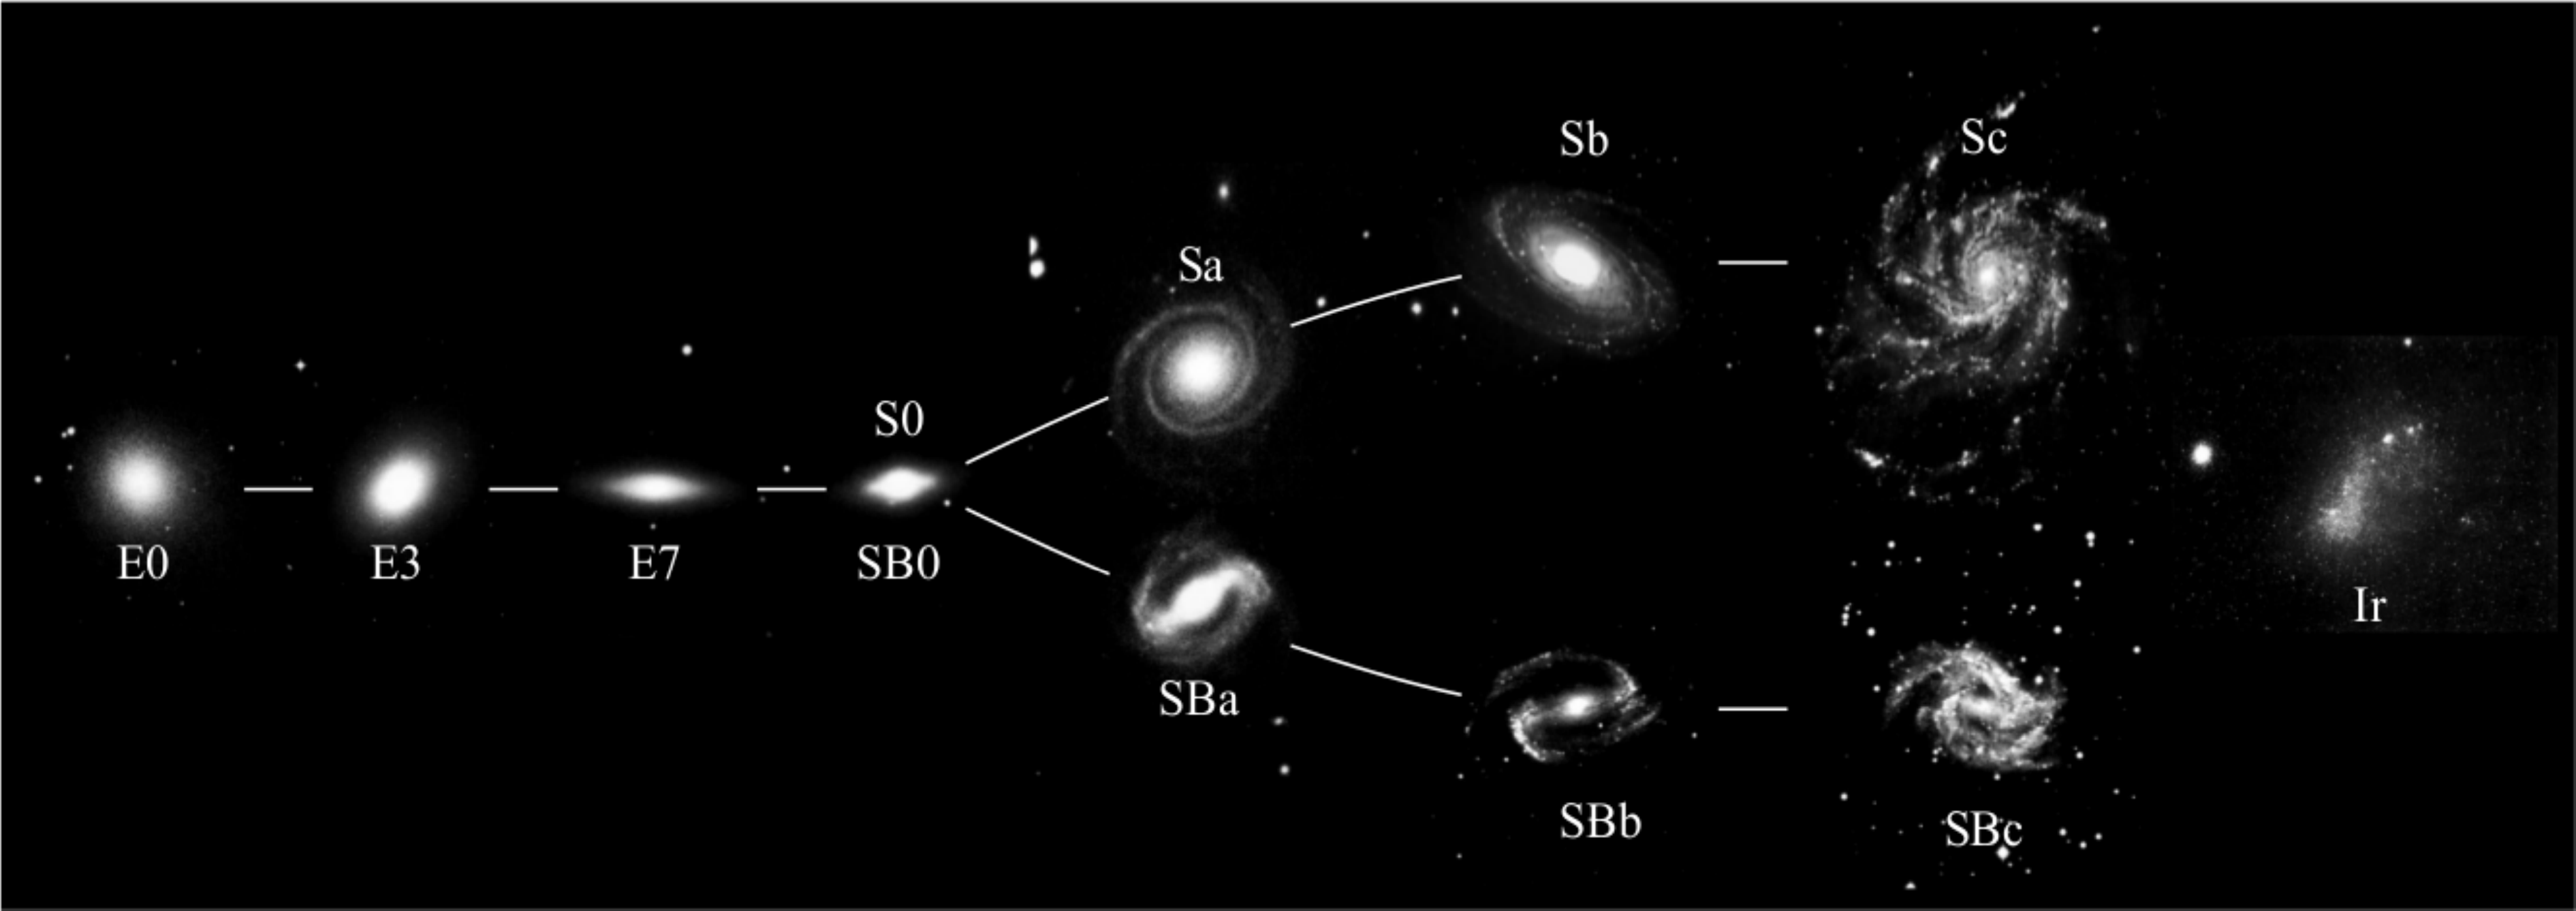
\includegraphics[width=12cm]{antecedentes/figures/hubble.png}
\end{center}

\begin{itemize}
\item Galaxias elípticas
\item Galaxias espirales
\end{itemize}

\note{
- Clasificacion morfologica o \textbf{secuencia de Hubble} \\
- galaxias elípticas (\textbf{E0-E7}) \\
- rama superior galaxias espirales sin barra \\
- rama inferior galaxias espirales con barra \\

}

\end{frame}

\begin{frame}
\frametitle{Componentes de una galaxia}

\begin{columns}
\column{0.3\textwidth}
\begin{center}
    \begin{itemize}
    \item Esferoide
    \begin{itemize}
        \item Bulge
        \item Halo
    \end{itemize}
    \item Disco
    \begin{itemize}
        \item Disco delgado
        \item Disco grueso
    \end{itemize}
\end{itemize}
\end{center}
\column{0.7\textwidth}
\begin{center}
    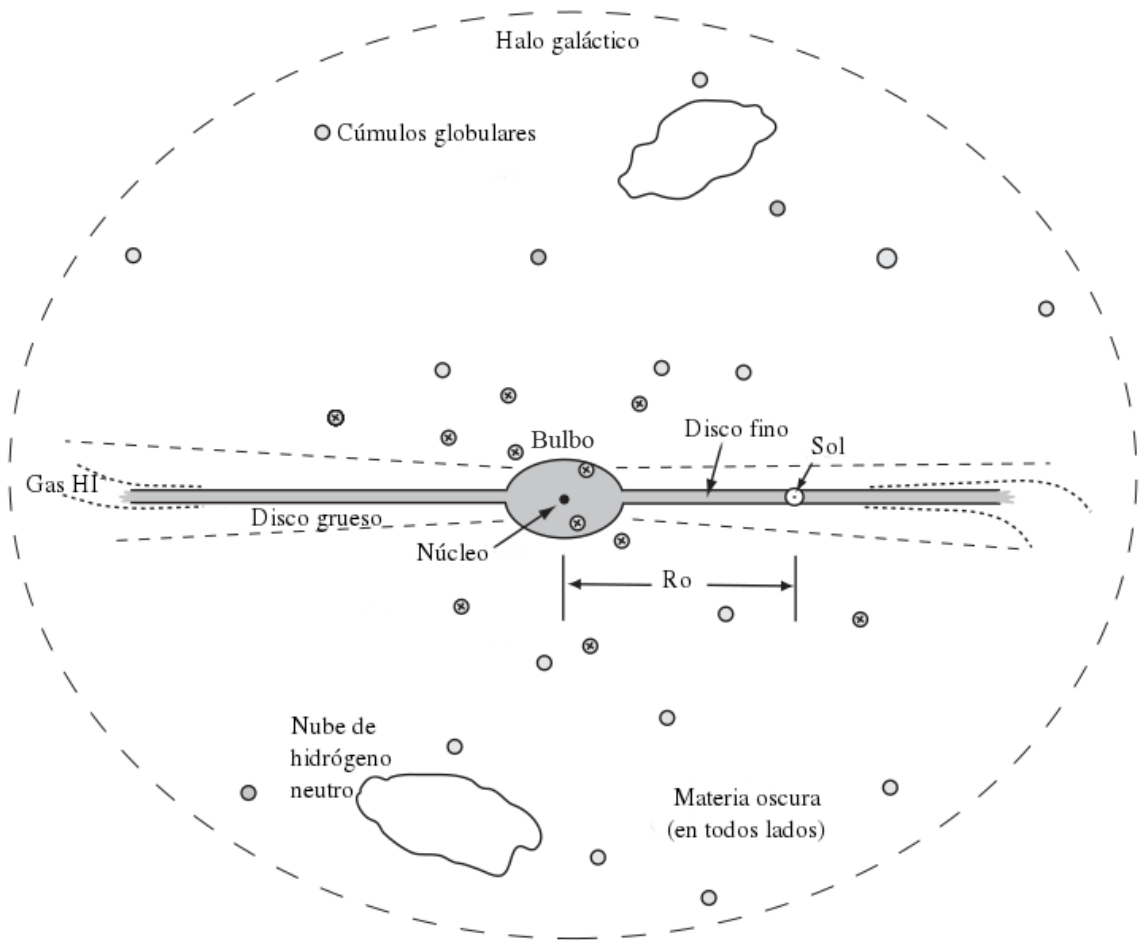
\includegraphics[width=8cm]{antecedentes/figures/mwschema.png}
\end{center}
\end{columns}

\note{
%\begin{itemize}
%\item Esferoide:
%    \begin{itemize}
%    \item Compuesto por una población estelar \textbf{roja} y vieja
%    \item Desde el punto de vista dinámico, las \textbf{estrellas del esferoide se encuentran soportadas por dispersión de velocidades, aunque puede presentar una rotación mínima}.
%    \item Subdivision
%    \end{itemize}
%\item Disco: 
%    \begin{itemize}
%    \item Compuesto principalmente por estrellas jóvenes, gas y polvo
%    \item Este es la componente principal de las galaxias espirales y lenticulares en lo que respecta a su masa.
%    \item Presenta una mayor tasa de formación estelar respecto al esferoide, debido a la existencia de gas en forma de hidrógeno, resultando en un color más azul gracias a la presencia de estrellas jóvenes
%    \end{itemize}
%\end{itemize}
}

\end{frame}




\begin{frame}
\frametitle{Problema observacional}

% 2.2.1 problemas de observacion al ver estrellas en x, y, z se puede confundir

\begin{center}
    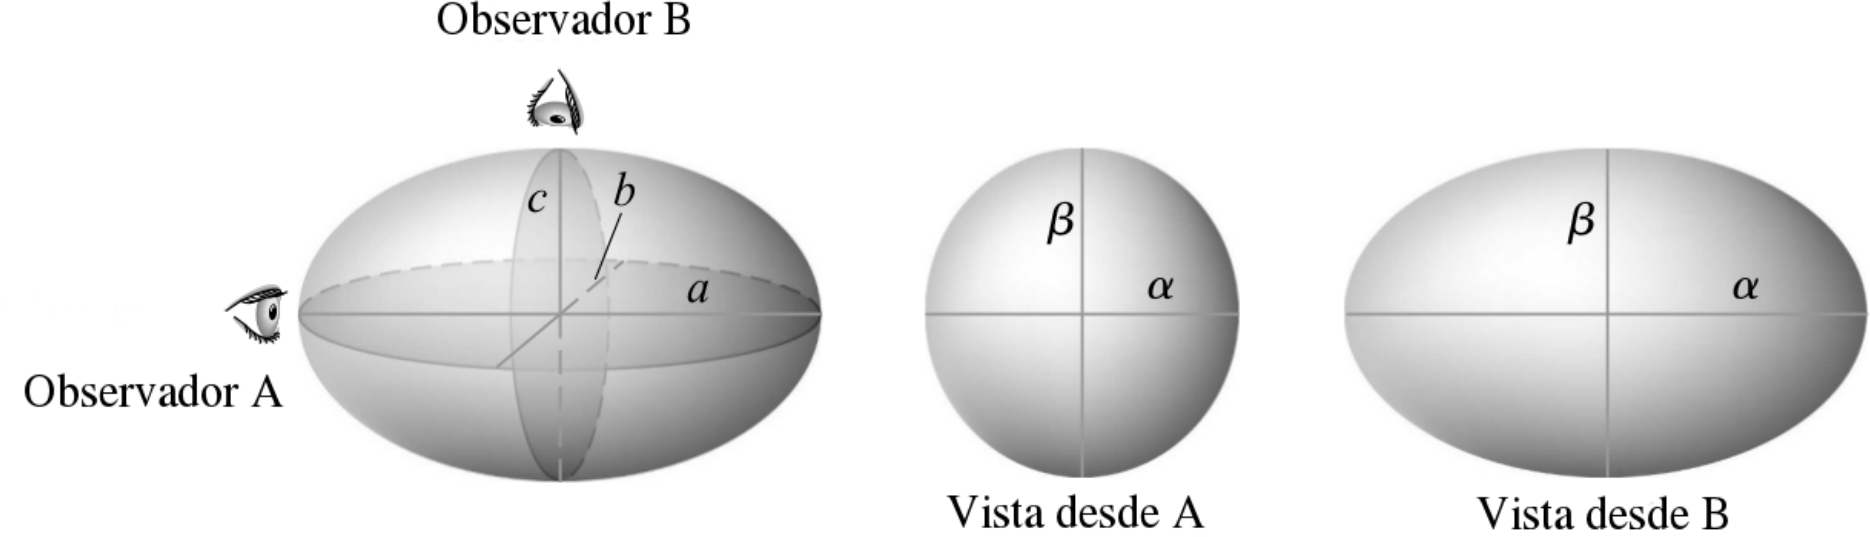
\includegraphics[width=12cm]{antecedentes/figures/proyecione_galactica.png}
\end{center}

\note{
\begin{itemize}
%\item Una galaxia elíptica con semiejes $a > b = c$,  observadores diferentes situados en diferentes posiciones percibirán diferentes formas proyectadas de este objeto, y consecuentemente la \textbf{clasificación} de particulas estelares \textbf{variará en cada caso}.
\item Problema en una proyección una estrella podría parecer que está en el esferoide mientras que \textbf{en realidad está en el disco}.
\item El area ha enfocado sus \textbf{esfuerzos en las características dinámicas de estrellas} en las componentes
%\item Requerimos de disponer de las posiciones y velocidades de las estrellas individuales que la conforman
%   \begin{itemize}
%    \item excede capacidades de telescopios actuales, por eso simulaciones
%    \end{itemize}
\item Estas caracteristicas (posiciones y velocidades de estrellas) no se pueden obtener con \textbf{telescopios actuales}, por lo cual \textbf{recurrimos a las simulaciones}
\end{itemize}
}

\end{frame}



\begin{frame}
\frametitle{Simulaciones}

\begin{center}
    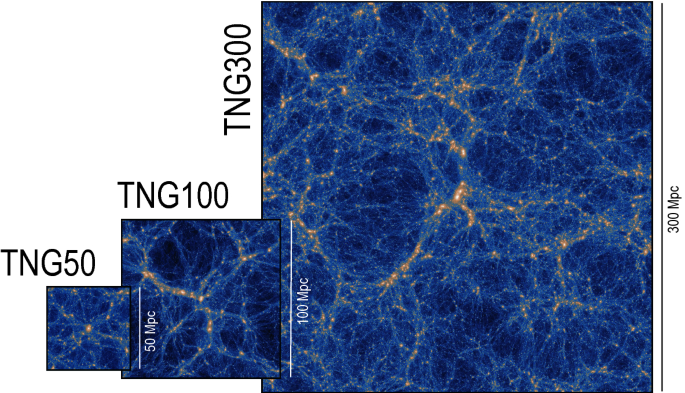
\includegraphics[width=12cm]{antecedentes/figures/tng.png}
\end{center}

\note{
- Estas simulaciones nos brindan la posibilidad de acceder a esta información. \\
- Estado del arte %en cuanto a combinar una alta resolución numérica con volúmenes computacionales cosmológicos suficientemente grande para que incluyan decenas de miles de galaxias individuales.
}

\end{frame}



\begin{frame}
\frametitle{Parámetros}

\begin{itemize}
    \item<2-> Parámetro de circularidad ($eps$):
        \[\epsilon = \frac{J_{z}(E)}{J_{circ}(E)}\]
    \item<3-> Parámetro de circularidad proyectada ($eps\_r$):
    \[\epsilon_{r} = \frac{J_{p}(E)}{J_{circ}(E)}\] Donde $J_P = \sqrt{J_x^2 + J_y^2}$
        
    \item<4-> Energía estelar normalizada ($normalized\_star\_energy$):
        \\
        \begin{center}
            $E/|E|_{max}$
        \end{center}
\end{itemize}

\note{
\begin{itemize}
\item<1-> Así, los tres valores que representan los movimientos de una partícula estelar y definen su ubicación en alguna de las componentes son \\
\item<2-> eps: Cuán \textbf{parecida} es la órbita de una partícula respecto a una \textbf{órbita circular}, para un dado valor de energía. %Es el cociente entre la componente z del \textbf{momento angular} y el momento angular que tendría una partícula, si utilizase toda su energía cinética para moverse en una órbita circular. \\
\item<3-> eps\_r: Representa la \textbf{dispersión vertical} del movimiento de una partícula con respecto al \textbf{plano} en el que se ubican las \textbf{partículas} que se mueven en \textbf{órbitas circulares}. %Donde $J_x$ y $J_y$ son las componentes restantes del vector momento angular de la partícula estelar. \\
\item<4-> norm: \textbf{que tan ligada} esta la particula a la galaxia%Cociente entre los valores de energía de las partículas estelares y el módulo de la energía de la partícula más ligada de la galaxia. \\
\item<4-> Las partículas más ligadas al sistema van a adoptar valores cercanos a -1, mientras que las menos ligadas van a  tener valores cercanos a 0.
\end{itemize}
}

\end{frame}



\begin{frame}
\frametitle{Métodos Establecidos}

\begin{itemize}
    \item Abadi
    \item Auto-Gaussian Mixture Model (AGMM)
\end{itemize}

\begin{center}
    
\includegraphics[width=12cm]{antecedentes/figures/galaxychop_logo.png}
    \href{https://github.com/vcristiani/galaxy-chop}{https://github.com/vcristiani/galaxy-chop}
\end{center}

\note{
- Abadi: Usa \textbf{eps} para separar en \textbf{Disco} y \textbf{Esferoide}. Asume que la componente esferoidal no presenta rotación y por lo tanto está representada por una distribución simétrica respecto de $\epsilon = 0$. Para ello selecciona el mismo número de partículas en órbitas corrotantes que aquellas que se encuentran en órbitas contrarrotantes. Luego, la distribución de las partículas restantes, se asignará al disco. Esto se debe a que el método asume que el disco está formado por partículas cuyo movimiento predominante es el de rotación. Como reflejo de esto, las partículas asignadas al disco tendrán $\epsilon \sim 1$. \\
- AGMM: Realiza \textbf{distribuciones Gaussianas} que representan las estructuras a ser identificadas, utilizando \textbf{$eps$, $eps_r$ y $normalized_star_energy$}. Genera dichos modelos variando el \textbf{número de componentes a buscar de 2 a 9}. En cada iteración, se crean 10 modelos con diferentes inicializaciones para alcanzar resultados más estables. El algoritmo usa una función a minimizar y un valor de disparo previamente establecido. Como la iteración comienza con 2 grupos y crece desde ahí, se tiene preferencia en buscar pocas componentes.
}

\end{frame}

\iflong
\begin{frame}
\frametitle{Aprendizaje automático}
\centering ¿Que es Machine Learning?

\pause

\vspace{0.5cm}

\begin{displayquote}
\textit{Se dice que un programa de computadora aprende de la experiencia $E$
respecto a una tarea $T$ y una medida de desempeño $P$, si el desempeño medido con $P$ en una tarea $T$, mejora con la experiencia $E$.}
\end{displayquote}

\note{
- La \gls{AI} tiene diferentes ramas siendo la de éxito actual aquella que postula que se puede imitar la inteligencia humana por medio del aprendizaje. En otras palabras, podemos brindar datos de ejemplo a un programa para que entienda su ``forma'' y generalice en una tarea dada. \\
- El \gls{ML} es un proceso inductivo para la exploración de conocimiento, donde su enfoque reside en la búsqueda de información general a partir de observaciones específicas que sesgan las suposiciones de conocimiento concreto, con el propósito de establecer una base sólida para realizar generalizaciones. 
}

\end{frame}
\fi


\iflong
\begin{frame}
\frametitle{Tipos de Aprendizaje Automático}

\begin{itemize}
    \item<1-> Aprendizaje Supervisado
    \item<2-> Aprendizaje No-Supervisado
\end{itemize}

\note{
%- Todos los métodos de \gls{ML} requieren datos de entrenamiento para adquirir conocimiento. Sin embargo, diversos tipos de tareas ($T$), experiencias ($E$) y desempeños ($P$) conducen a múltiples especializaciones. La clasificación inicial más común categoriza a los modelos de \gls{ML} en función de cómo el algoritmo utiliza o no valores objetivos a aproximar: \\
%- Supervisado: Aproxima la función $F(X) = y$, con $X$ como datos de entrada o matriz de \textit{features} y el vector $y$ corresponde a sus respectivas etiquetas o clases objetivos. Puede tomar la forma de un conjunto finito de etiquetas discretas (clasificación) o intentar predecir un valor numérico real que represente alguna magnitud (regresión). \\
- Supervisado: Utiliza un \textbf{conjunto de entrada y salidas} para entrenar un \textbf{modelo} que se usara para predecir nuevas entradas. \\
- No supervisado: Adquiere conocimiento durante la ejecución de la tarea sin requerir etiquetas. \\%Ej reducción de la dimensionalidad, la visualización de datos (manteniendo sus propiedades fundamentales) o la agrupación en conjuntos con características similares. \\
%- Dos etapas: la de entrenamiento y la de predicción. Además, hay varios modelos que poseen hiperparámetros que pueden ser configurados previamente a la fase de entrenamiento. \\
- Falta de etiquetas en galaxias, vamos a hacer no supervisado
}

\end{frame}
\fi

\begin{frame}
\frametitle{Metodos de Clustering}

\begin{itemize}
    \item<2-> Métodos jerárquicos
    \item<3-> Métodos difusos/\textit{fuzzy}
    \item<4-> Métodos basados en acumulación de evidencia
\end{itemize}

\note{
\begin{itemize}
\item<1-1> Utilizaremos entonces metodos de Clustering (que son no-supervisados) para asignar las partículas estelares a las diferentes componentes galácticas. Los algoritmos de \textit{clustering} tienen la \textbf{tarea de agrupar un conjunto de objetos} de tal manera que los objetos de un mismo grupo (llamado \textit{cluster}) sean \textbf{más similares}, en algún sentido, entre sí \textbf{que los de otros} grupos ($clusters$). \\
\item<2-> Jerarquico: Crean agrupamientos basándose en agrupamientos más pequeños de una manera jerárquica. Buscamos reflejar\textbf{ estructura jerarquica de galaxia}. \\
\item<3-> Fuzzy: Dado que una partícula de varias masas solares \textbf{puede pertenecer a más de una componente} galáctica al mismo tiempo, queremos evaluar cómo se comporta los métodos de agrupamientos basados en \textbf{lógica difusa} para la asignación de la misma partícula en diferentes componentes. \\
\item<4-> EAC: Permiten \textbf{combinar y consensuar} resultados provenientes de otras técnicas de clustering. Para \textbf{busacar estructuras complejas} que no son posibles de encontrar en un solo metodo de agrupamiento.
\end{itemize}
}

\end{frame}






%saltear rapido
\begin{frame}
\frametitle{Métricas de validación externa}

\begin{columns}
\column{0.45\textwidth}
\begin{center}
    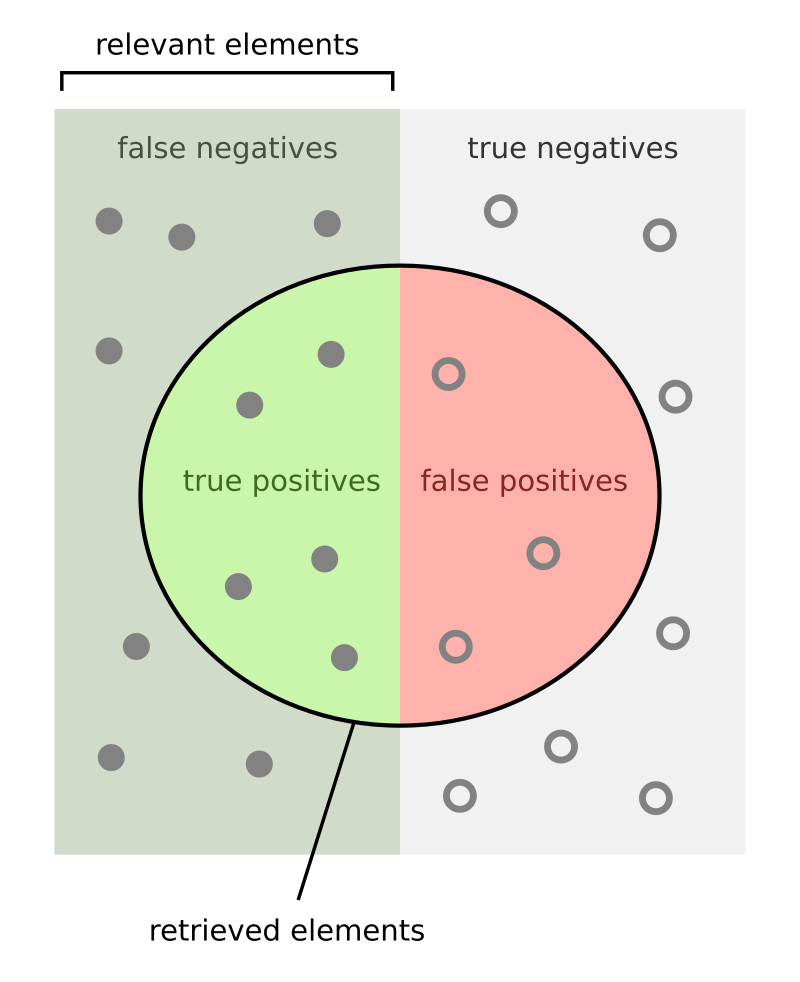
\includegraphics[width=6cm]{antecedentes/figures/Precisionrecall-1.png}
\end{center}
\column{0.7\textwidth}
\begin{center}
    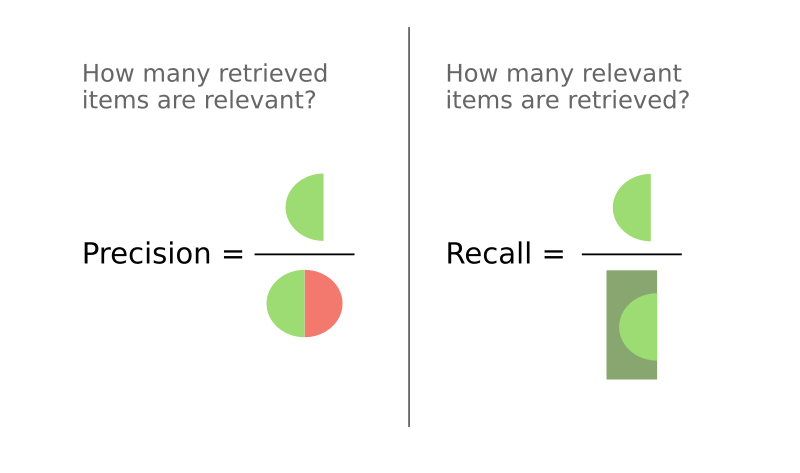
\includegraphics[width=8cm]{antecedentes/figures/Precisionrecall-2.png}
\end{center}
\end{columns}

%\begin{itemize}
%    \item<1-> Presicion
%    $$Precision = \frac{TP}{TP + FP}$$
%    \item<2-> Recall
%    $$Recall = \frac{TP}{TP + FN}$$
%\end{itemize}

%\begin{table}[]
%    \centering
%    \begin{tabular}{c|c|c}
%         {}                   & \multicolumn{2}{l}{\textbf{Clase Predicha}} \\
%         \textbf{Clase Real}  & \textbf{Positiva}  &  \textbf{Negativa}                        \\
%         \textbf{Positiva }            &  \gls{TP}       & \gls{FN}                               \\
%         \textbf{Negativa}             &  \gls{FP}       & \gls{TN}
%    \end{tabular}
%\end{table}

\note{
\begin{itemize}
\item Clustering \textbf{discierne grupos entre sí}, no los cataloga. Una vez \textbf{etiquetados los datos manualmente}, es necesario \textbf{compararlos} con los obtenidos con algún método que tengan una fundamentación física sólida y además provean estas etiquetas. Los resultados de estos metodos los llamaremos GT, y vendran de \textbf{Abadi} y \textbf{AGMM}. Teniendo el cuidado de utilizar los mismos parámetros dinámicos en cada caso. %Comparando los resultados de \gls{GT} y los del metodo a evluar, podemos crear la \gls{CM} (explicar con dos clases). 
\item Presicion:  Cuánto de lo que seleccioné era realmente relevante.  %La proporción de partículas bien asignadas a una componente respecto al total que fue asignada a esa componente. \\
\item Recall: Cuánto de lo relevante fue seleccionado. %La proporción de partículas bien asignadas a una componente respecto al total que debería haber sido asignado a esa componente.  \\
%\item Hacer \textbf{promedio pesado} para aplicar a todas las clases y lidiar con el desbalance de clases (ej flores?)
\end{itemize}
}

\end{frame}



\begin{frame}
\frametitle{Métricas de validación interna}

\begin{itemize}
    \item<1-> Puntaje de Silhouette (SSc)
    $$
    s(i)={\frac {b(i)-a(i)}{\max\{a(i), b(i)\}}}
    $$
    \begin{itemize}
    \item $a(i)$: promedio de la distancia entre el punto $i$ con todos los puntos del mismo cluster
    \item $b(i)$: promedio de la distancia entre el punto $i$ con todos los puntos del cluster más cercano
    \end{itemize}
    \item<2-> Índice de Davies–Bouldin (DBI) \\
    Busca para todos los \textit{clusters} $c_i$, el \textit{cluster} $c_j$ que maximiza el valor $R_{ij}$, para luego promediar todos los valores $R_{ij}$ obtenidos. 
    \begin{itemize}
        \item $s_i$: La distancia promedio de cada punto en el \textit{cluster} $c_i$ al centro de su mismo \textit{cluster}
        \item $d_{ij}$: Distancia entre los centros de los \textit{clusters} $c_i$ y $c_j$
        \item $R_{ij}$: La suma de $s_i$ y $s_j$ dividido $d_{ij}$
    \end{itemize}
\end{itemize}

\note{
- Utilizan todo el conjunto de datos que se usó para entrenar al modelo, y analizan la \textbf{distancia intra y extra \textit{cluster}}, y la continuidad espacial que tienen los datos dentro de sus clusters. Esto da una idea de la estructura interna sin necesidad de recurrir a valores externos. \\
- Silhouette: El puntaje es el promedio del coeficiente en cada punto. Valores $\sim 1$ \textit{clusters} están bien separados entre si y son a su vez bien compactos; valores $\sim -1$ existen puntos mal clasificados; $\sim 0$ existe una superposición entre \textit{clusters} \\
- Davies Bouldin: Valores $\sim 0$ mejor agrupamiento, valores alejados de $0$ (hasta infinito) dan a entender un mal trabajo de \textit{clustering}. \\
- Valores \textbf{alejados del ideal} no esta necesariamente mal, depende de la \textbf{naturaleza de los clusters}
}

\end{frame}








\begin{frame}
\frametitle{Análisis físicos del área}

Curva de Perfil de Velocidades
\begin{center}
    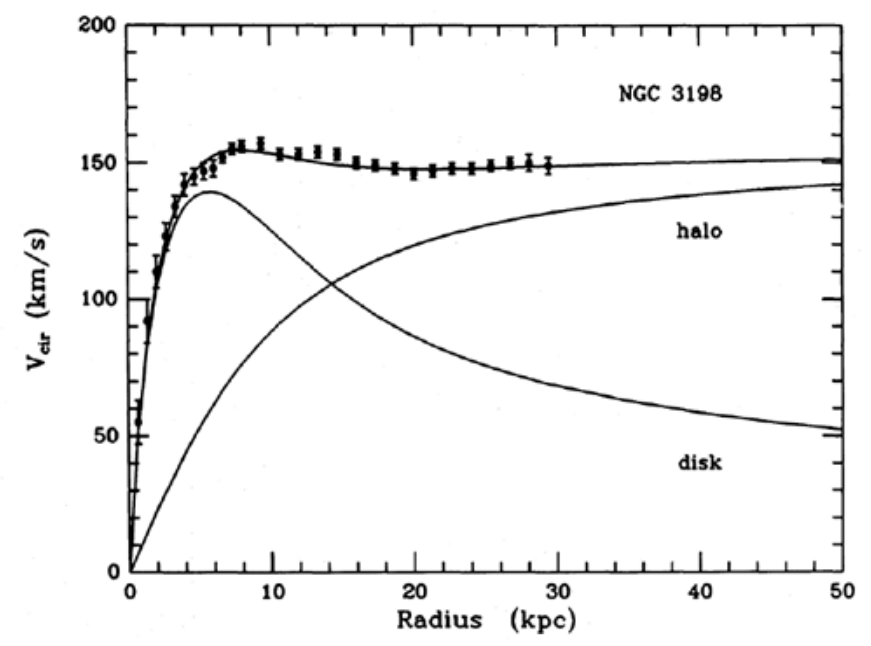
\includegraphics[width=8cm]{antecedentes/figures/vprofile.png}
\end{center}

\note{
%- Crear un puente hacia los astrónomos presentando los resultados en una forma que es habitual en el área. \\
%- Hay otras mas complejas, asi que usamos esta simple que podemos entender \\
- Muestran la \textbf{velocidad de rotación} de las componentes en una galaxia en función de su \textbf{distancia radial al centro} de las mismas. \\
%- por ej, las estrellas del disco se acumulan más cerca del centro de la galaxia, mientras que las partículas del halo predominan en la región más externa de la misma. Esperable para dichas componentes. \\
- Si \textbf{superponemos nuestras curvas} con \gls{GT}, ver si en la dinámica de las componentes identificadas se reproducen los comportamientos típicos estudiados en la física; esto lo vuelve una \textbf{métrica externa}.
}

\end{frame}




\begin{frame}
\frametitle{Remover Atípicos/Outliers}

\begin{itemize}
    \item<2-> Isolation Forest
    \begin{center}
        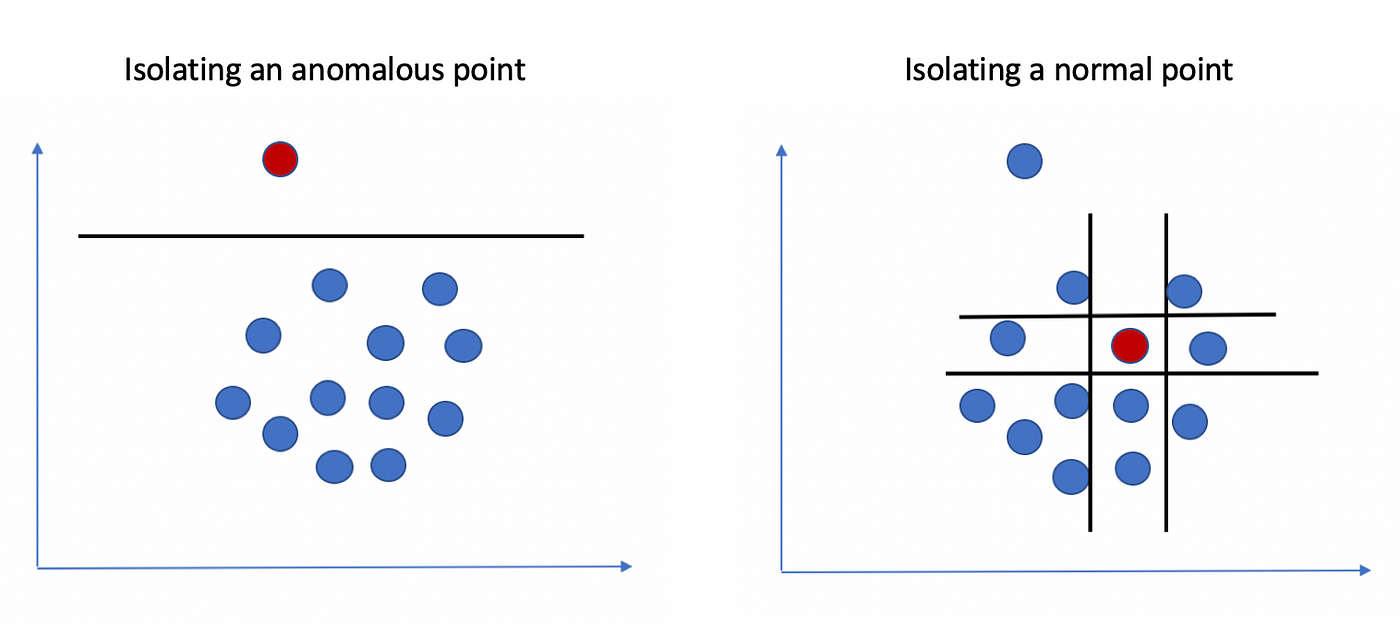
\includegraphics[width=8cm]{antecedentes/figures/isolation_forest.png}
    \end{center}
    \item<3-> RCut
\end{itemize}

\note{
\begin{itemize}
\item<1-> Podemos considerar atípicos a valores que están muy \textbf{alejados del centro galáctico} y puede que estén muy \textbf{débilmente ligados gravitacionalmente}
\item<2-> IF: Detecta anomalías mediante árboles binarios. Divide el espacio de datos mediante \textbf{líneas paralelas a la base canónica} y asigna puntuaciones de anomalía a los datos, con valores más altos a los puntos de datos que necesitan menos divisiones para ser aislados. %Para aislar un punto del resto de los datos, el algoritmo genera recursivamente particiones en la muestra seleccionando aleatoriamente un atributo, para luego seleccionar también de forma aleatoria un valor de partición entre los valores mínimo y máximo permitidos por ese atributo. Aplicado sobre las coordenadas en el espacio real de cada partícula estelar, en lugar de utilizar los parámetros de circularidad descritos anteriormente.
\item<3-> RCut: Desde el punto de vista de la astrofísica, es habitual considerar a las galaxias como las partículas estelares con radio $r <= X Kpc$, donde $X$ es 3 veces el radio que encierra la mitad de la masa estelar. Esta heurística es usada en diversos trabajos como una \textbf{forma rápida de descartar valores} que es poco probable que pertenezcan a la galaxia, pero que el algoritmo que identifica las galaxias las haya asignado allí.
\end{itemize}
}

\end{frame}



\begin{frame}
\frametitle{Recursos computacionales}

Recursos computacionales proveídos por:

\begin{columns}
\column{0.5\textwidth}
\begin{center}
    
\includegraphics[width=6cm]{antecedentes/figures/IATE-01.png}
\end{center}
\column{0.5\textwidth}
\begin{center}
    
\includegraphics[width=6cm]{antecedentes/figures/ccad_solo_new.png}
\end{center}
\end{columns}

\begin{center}
    
\includegraphics[width=6cm]{antecedentes/figures/cenits.jpg}
\end{center}

\note{
- Algoritmos son \textbf{caros computacionalmente y en memoria} con la gran cantidad de datos que analizamos, por lo cual requerimos de supercomputadoras para correrlos. \\
- \textbf{Instituto de Astronomía Teórica y Experimental}, y el \textbf{Centro de computacion de alto desempeño} de la Universidad Nacional de Córdoba \\
- \textbf{Centro Extremeño de Investigación, Innovación Tecnológica y Supercomputación}, que forman parte de la Fundación Computación y Tecnologías Avanzadas de Extremadura de la \textbf{Red Española de Supercomputación}.
}

\end{frame}

\section{Clustering Jerárquico}

\begin{frame}

\frametitle{Clustering Jerárquico}

\pause

%Tipos de clustering jerárquico:
%\begin{itemize}
%\item Aglomerativas
%\item Divisivas
%\end{itemize}

\begin{center}
    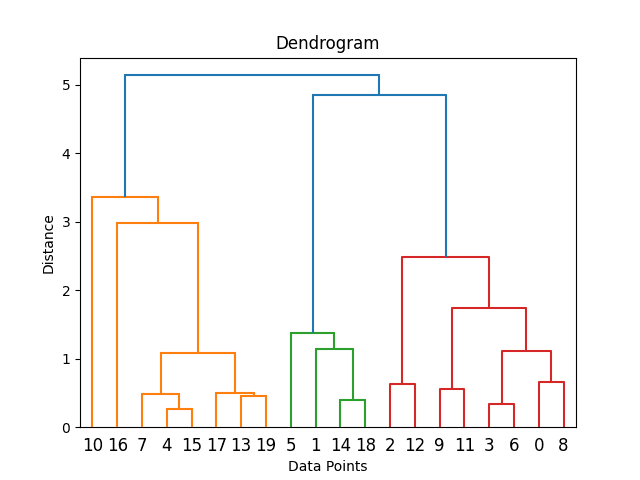
\includegraphics[width=9cm]{clustering jerarquico/figures/hierarchical-clustering-dendogram}
\end{center}

\note{
\begin{itemize}
\item <1-> Familia de algoritmos que buscan en los datos \textbf{grupos organizados jerárquicamente}. Así, a medida que se aumenten la cantidad de clusters buscados, estos se irán dividiendo o fusionando hasta alcanzar el número deseado
%\item <1-> Galaxias estructura jerarquica
\item <2-> Cada observación comienza en su propio grupo, y los pares de grupos son mezclados mientras uno sube en la jerarquía. \\
%\item <2-> Divisivas: Este es un acercamiento descendente. Todas las observaciones comienzan en un grupo, y se realizan divisiones mientras uno baja en la jerarquía.
\item <2-> Para poder decidir qué grupos deberían ser combinados o cuando un grupo debería ser dividido se requiere una \textbf{medida de disimilitud} entre conjuntos de observaciones. Esta medida es llamada \textbf{linkage}, y la libreria utilizada tiene las siguientes disponibles:
\end{itemize}
}

\end{frame}



\begin{frame}
\frametitle{Tipos de linkage}

\begin{itemize}
\item <1-> Ward
\item <2-> Complete
\item <3-> Average
\item <4-> Single
\end{itemize}

\note{
\begin{itemize}
    \item <1-> Ward: Minimiza la \textbf{suma de las diferencias al cuadrado dentro} de todos los clusters. Es un enfoque de \textbf{minimización de la varianza}.
    \item <2-> Complete: Minimiza la \textbf{distancia máxima entre observaciones} de pares de clusters.
    \item <3-> Average: Minimiza la \textbf{media de las distancias} entre todas las observaciones de pares de conglomerados.
    \item <4-> Single: Minimiza la distancia entre las observaciones \textbf{más cercanas de pares} de conglomerados.
    \item <5-> Usamos \textbf{aglomerativo} ya que parece ser el que mejores resultados da en el área de estudio \\
    %- Usamos distancia euclidiana, dado que los dominios de los datos con los cuales trabajamos son continuos \\
    \item <5-> Para \textbf{decidir sobre el linkage} a utilizar realizamos los experimentos descritos a continuacion
\end{itemize}
}

\end{frame}




\begin{frame}
\frametitle{Librería utilizada}

\begin{center}
    
\includegraphics[width=7cm]{clustering jerarquico/figures/Scikit_learn_logo_small.svg.png}
\end{center}

\vspace{0.5cm}

\center \href{https://scikit-learn.org/stable/}{https://scikit-learn.org/stable/}

\end{frame}




\begin{frame}
\frametitle{Selección de linkage}

\begin{center}
    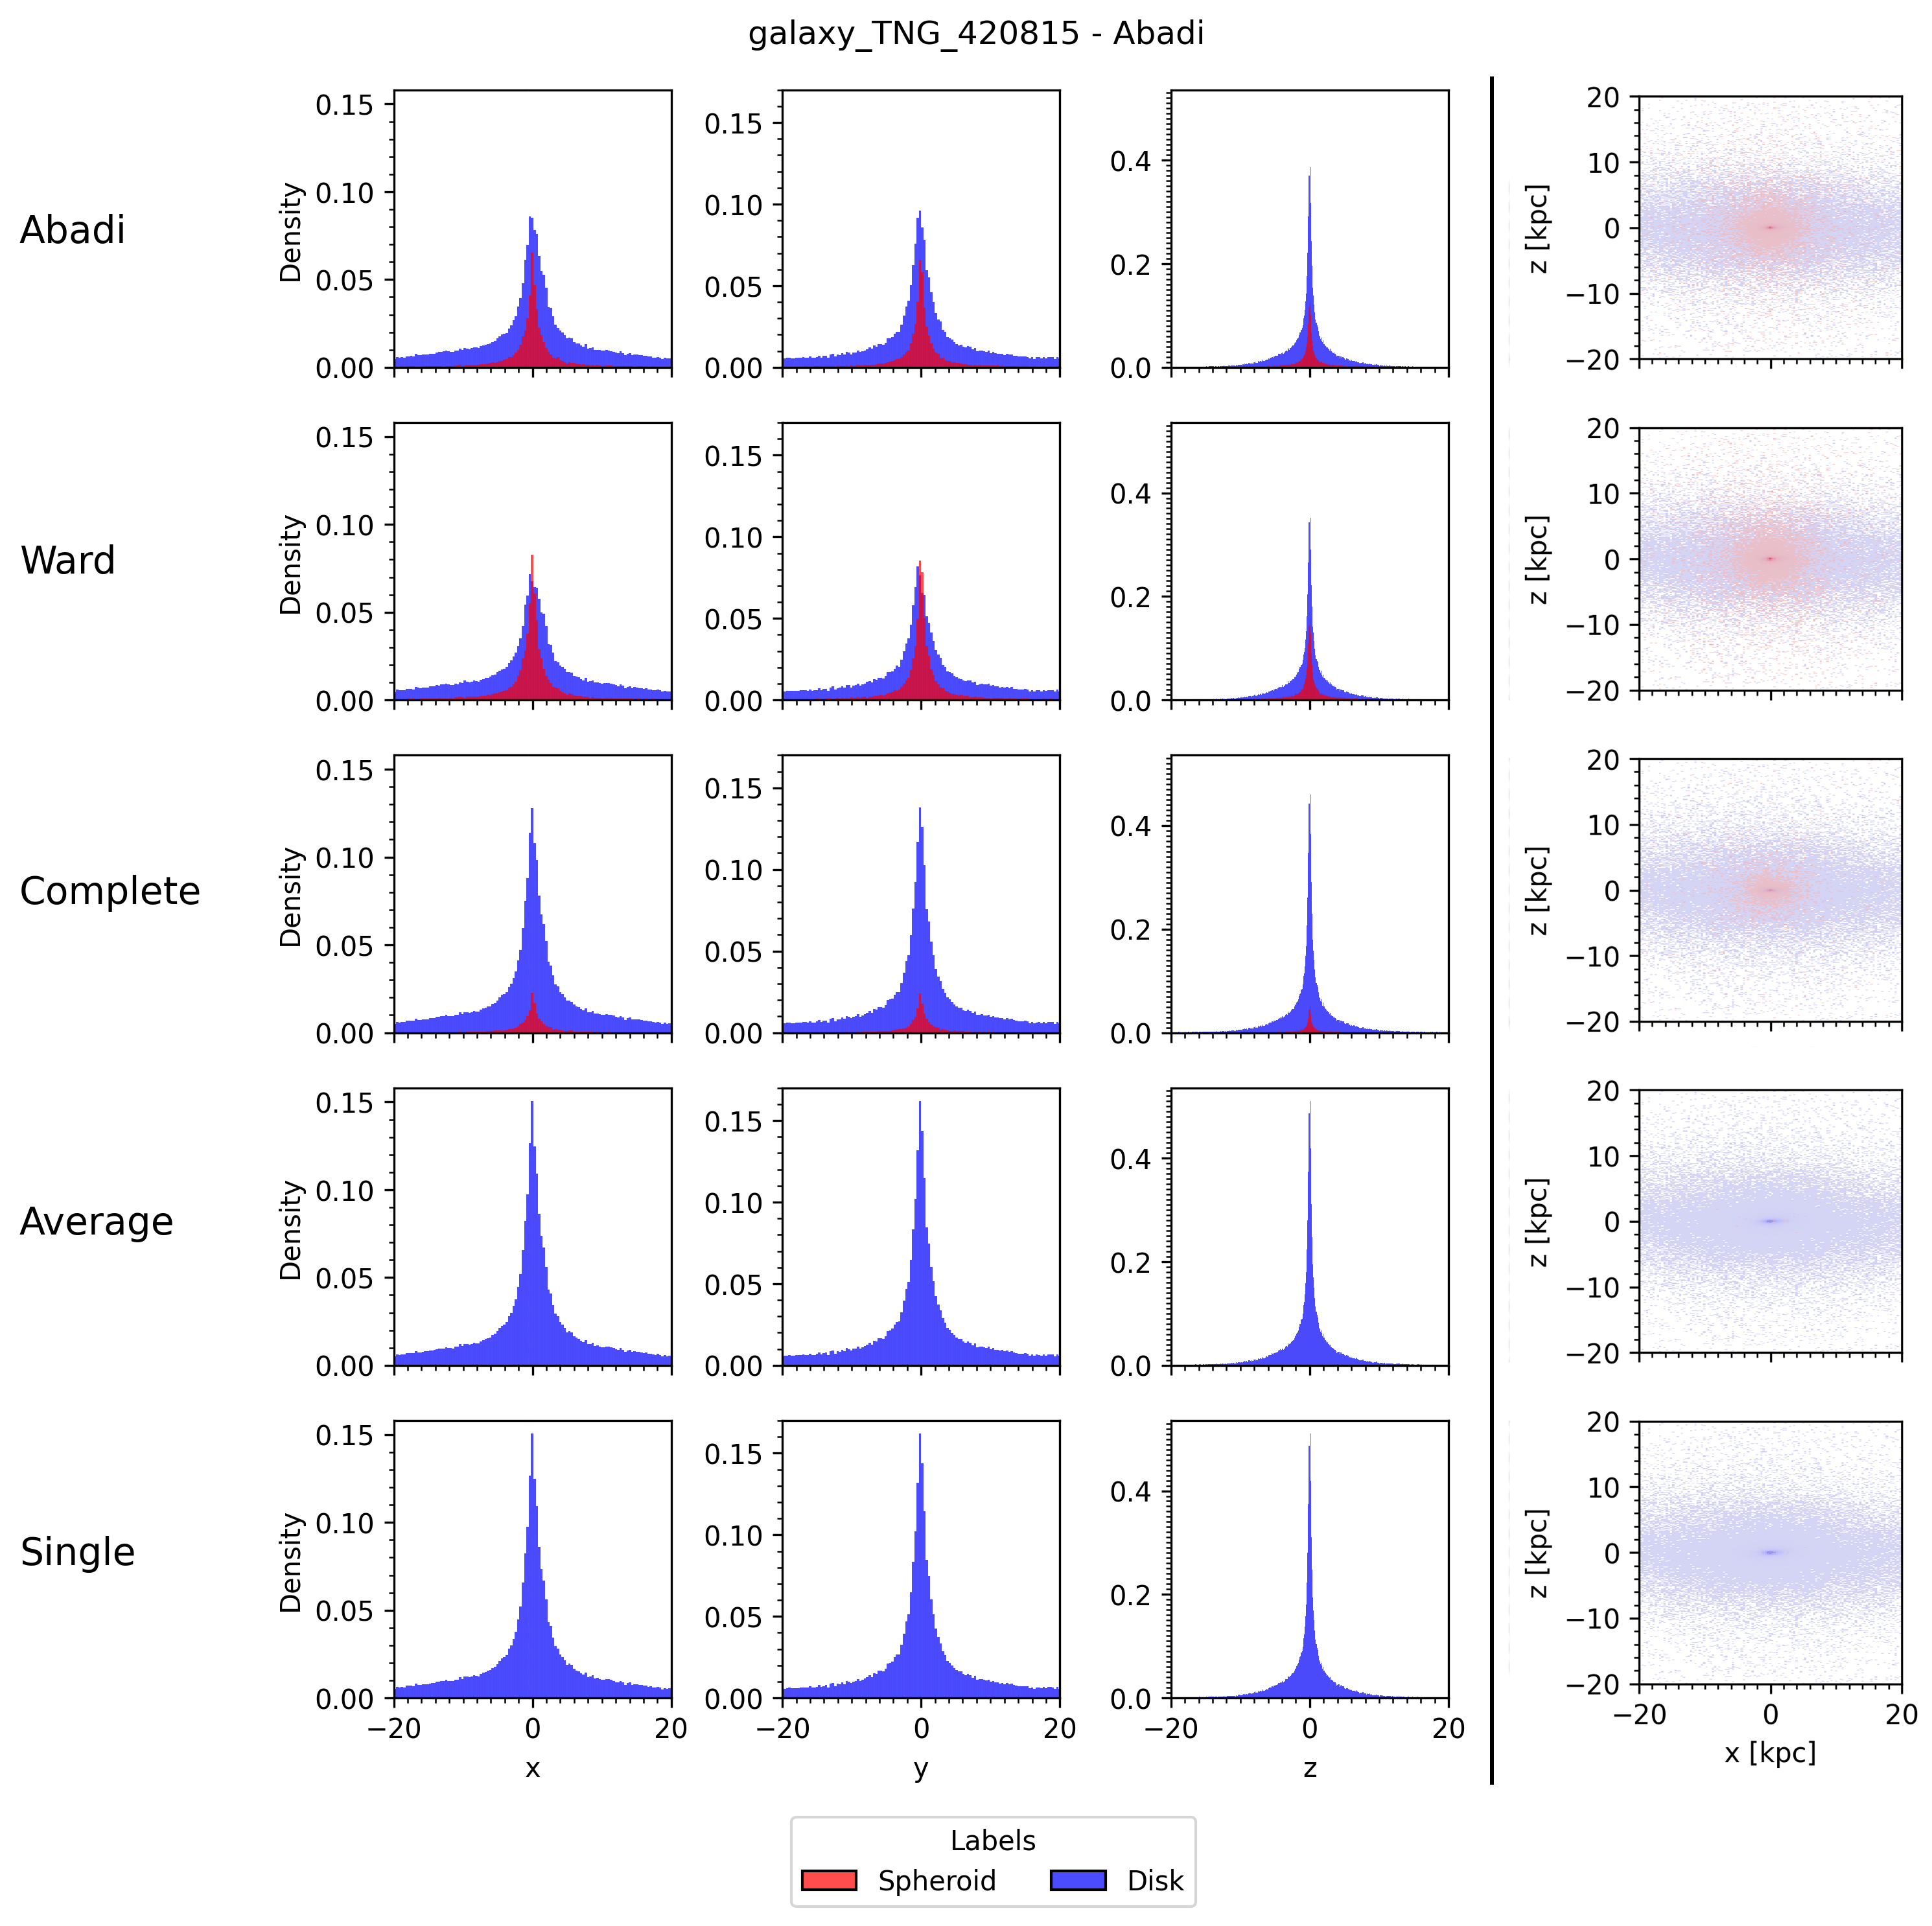
\includegraphics[width=7cm]{clustering jerarquico/figures/linkage_comparison.png}
\end{center}

\note{
- Aplicamos todos los linkages y comparamos con el método de Abadi, sobre un conjunto de 9 galaxias. \\
%- Ward da bien, puede ser por el uso de \textbf{el enfoque de las distancia intra-clusters} sea una métrica mucho más consistente e inmune al ruido en comparación al resto. \\
%- Average y Single pusieron casi todo en la \textbf{misma componente}.\\% Porque las partículas estelares de diferentes \textbf{componentes} en el espacio de circularidad están tan cercanas entre ellas que encontrar clusters se ve dificultado. \\
%- Single el cual hace uso de la distancia mínima inter-clusters, basta con tener un solo punto alejado del resto de nuestros datos para que éste sea identificado como un único cluster. \\
%- Average: su tarea se ve perjudicada por el alto solapamiento de los clusters \\
%- Complete: si bien da algunos resultados similares a Abadi, es \textbf{inestable} y no logra resultados con la consistencia que logra Ward en el apendice \\
}

\end{frame}

%capaz mostrar lo cerca que estan las particulas en cada feature?


\begin{frame}
\frametitle{Abadi: Detección de 2 componentes}

\begin{center}
    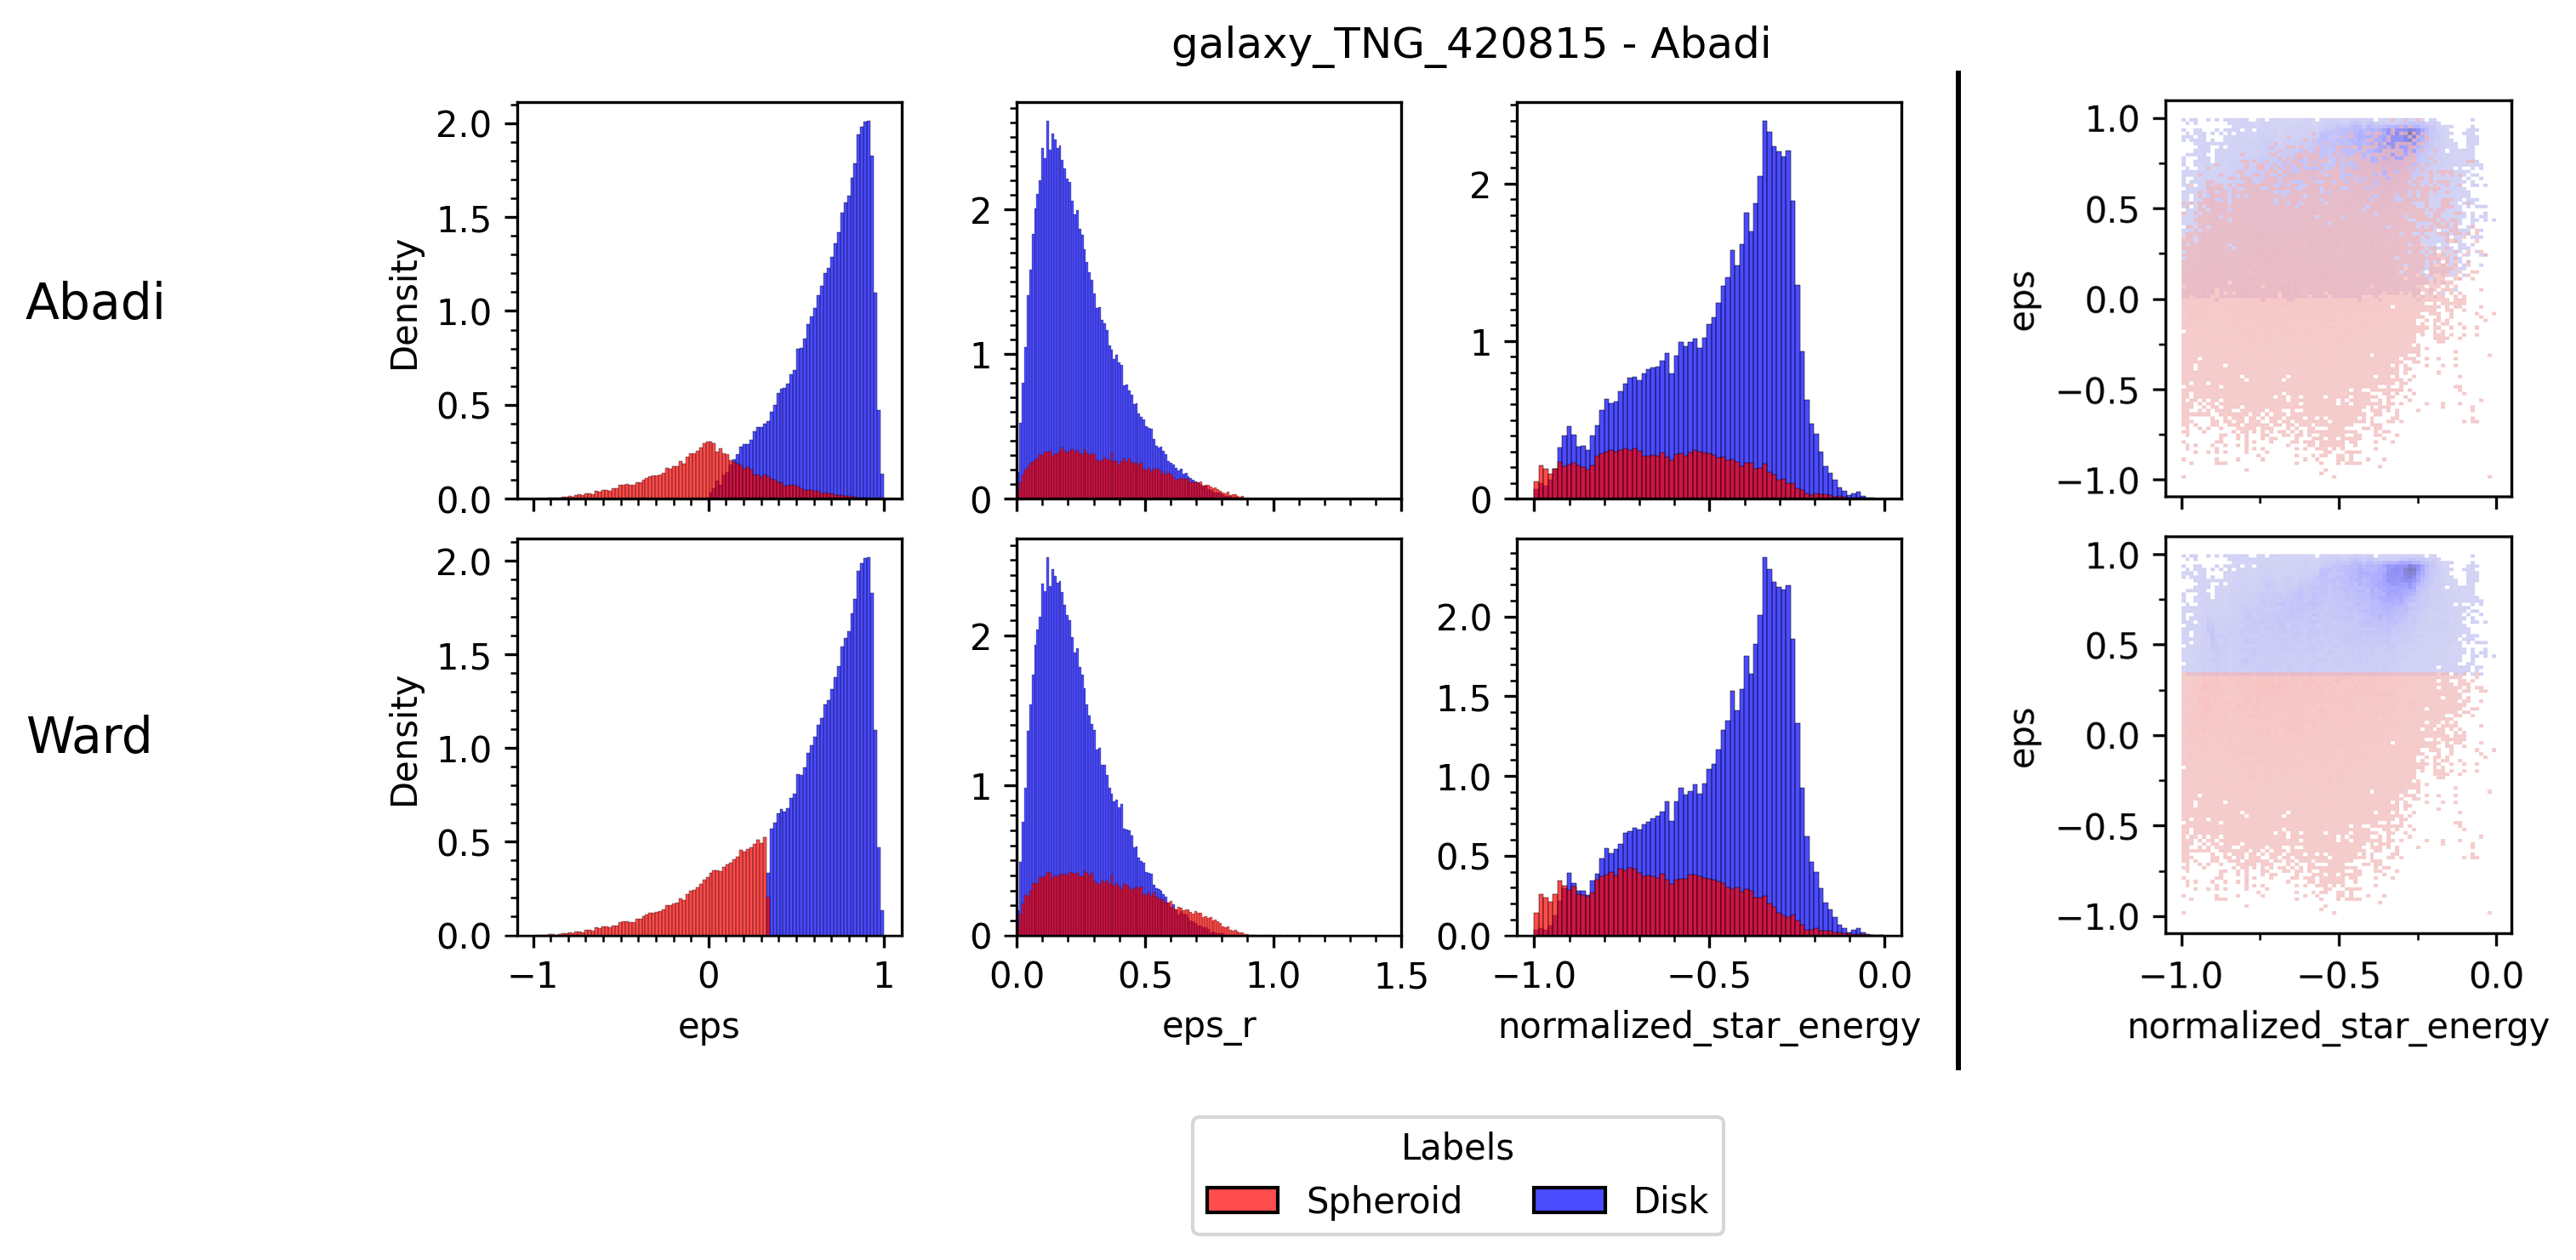
\includegraphics[width=8cm]{clustering jerarquico/figures/galaxy_TNG_420815 - abadi - base - circ histogram and scatterplot.png}
    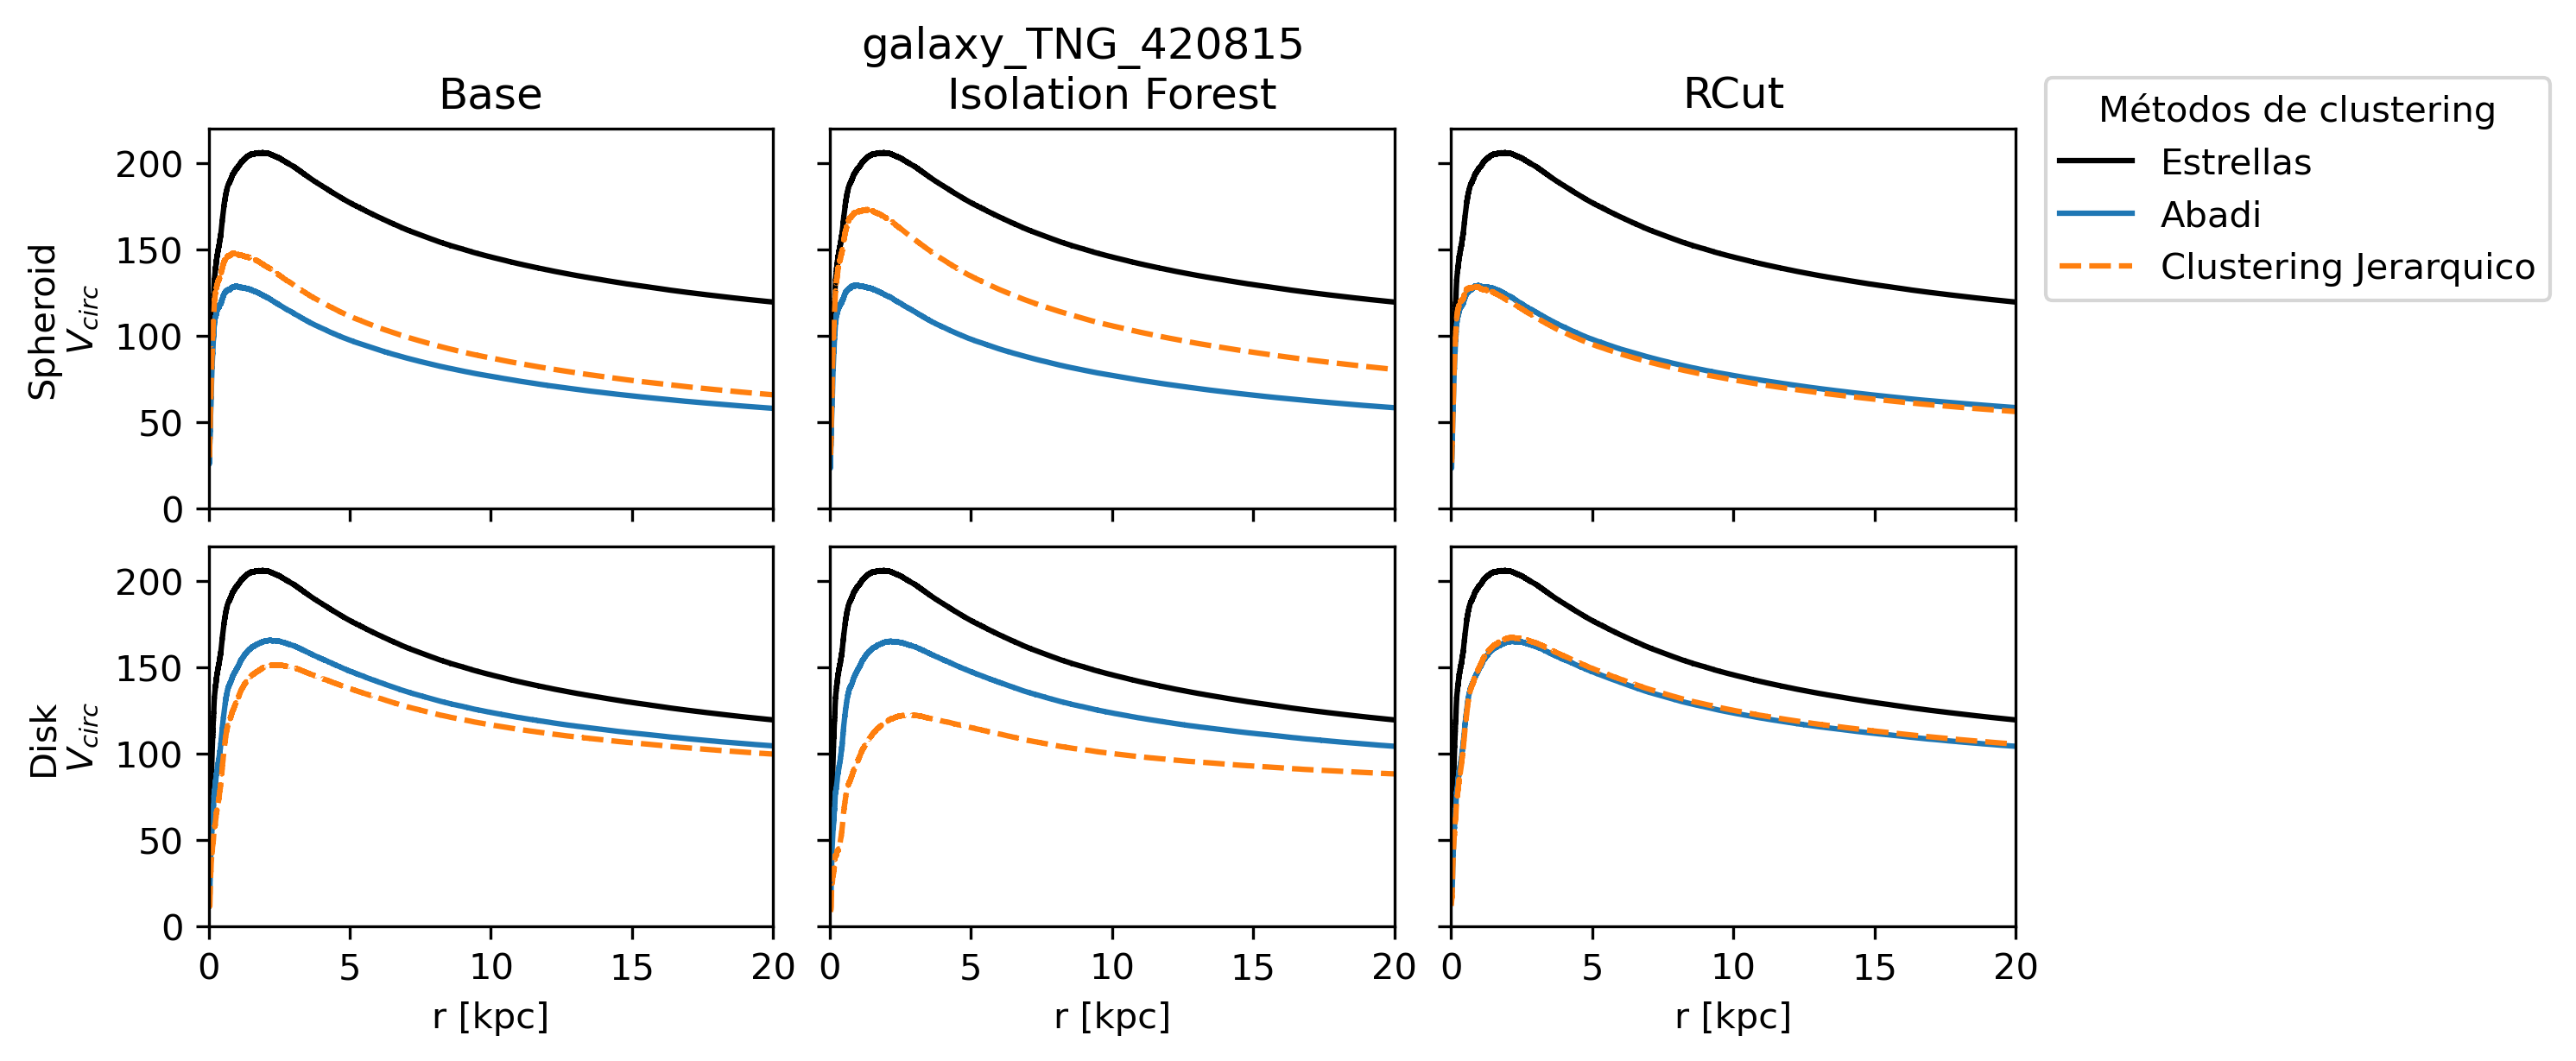
\includegraphics[width=8cm]{clustering jerarquico/figures/galaxy_TNG_420815 - Abadi - circ_velocity.png}
\end{center}

\note{
%- parametro vs feature \\
- recordamos que se usan las \textbf{mismas features que Abadi}, buscando 2 clusters \\
- \textbf{corte en vertical} feo por falta de heuristica, es el \textbf{mejor resultado} al cual se puede aspirar\\
- Esta situación hace que haya una \textbf{sobreestimacion del esferoide} como se ve en los perfiles de velocidad \\
}

\end{frame}




% presicion y recall
%bastante bien (penultimo parrafo de seccion 3.2
% los resultados parecen converger a los de abadi
%podria ser mejor (ultimo parrafo seccion 3.2)



%\begin{frame}
%\frametitle{Abadi: Eliminación de outliers}

%\begin{center}
%    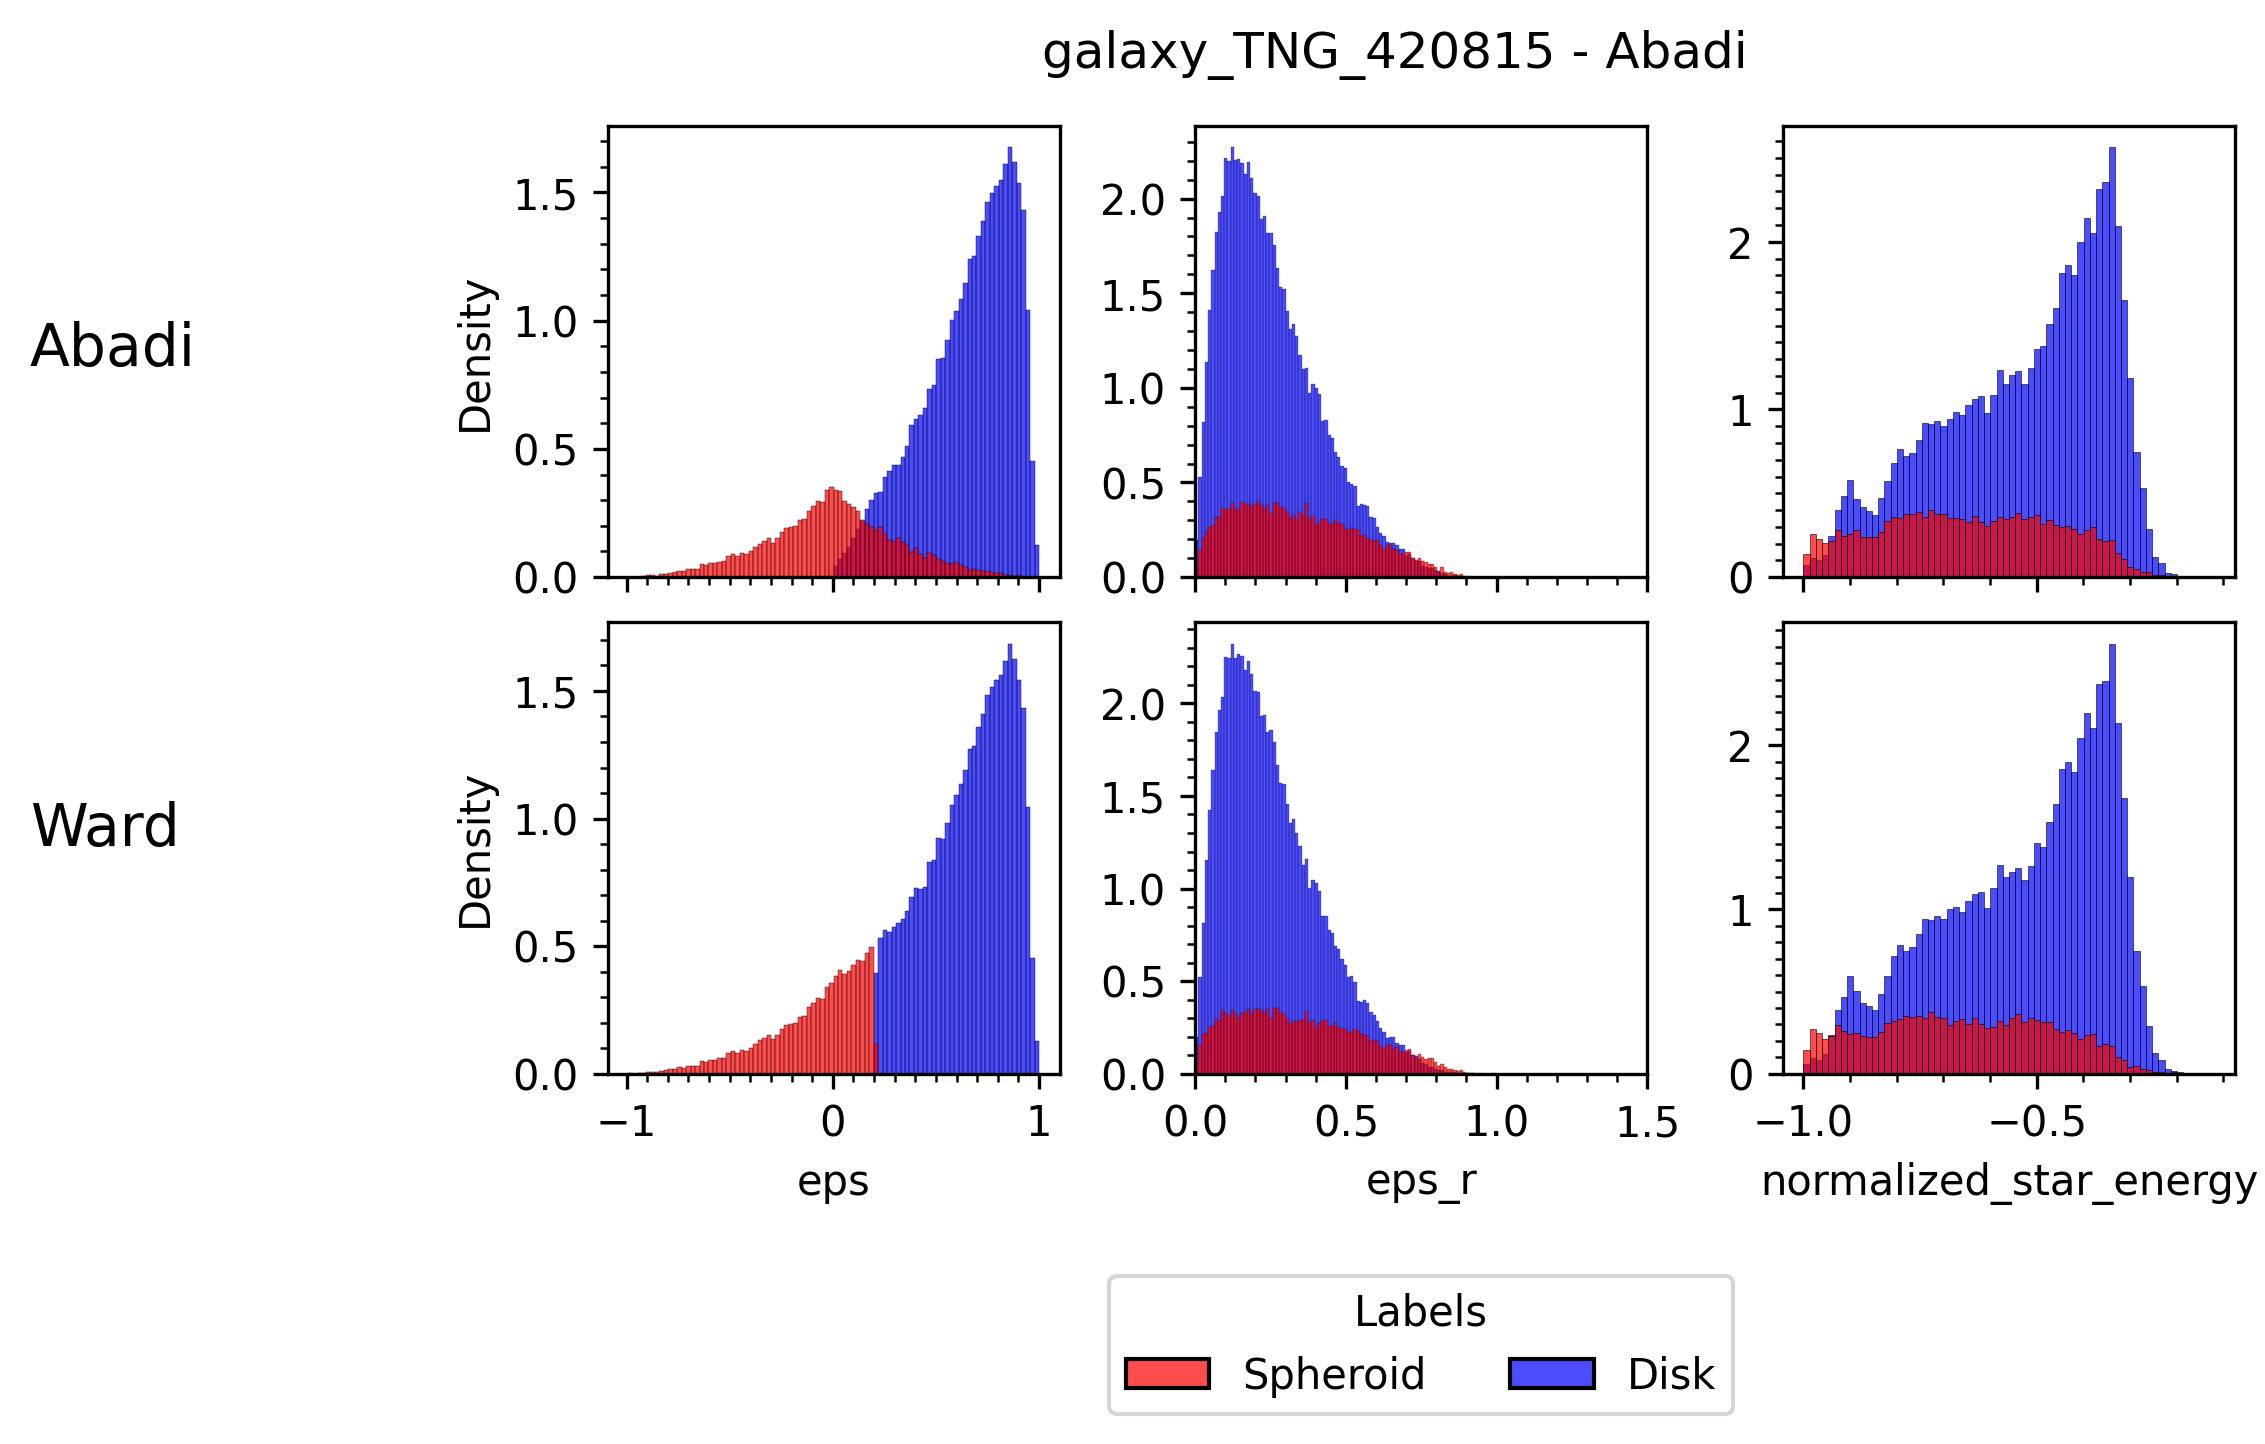
\includegraphics[width=12cm]{clustering jerarquico/figures/galaxy_TNG_420815 - abadi - rcut - circ histogram.png}
%\end{center}

%\note{
%Esto que vemos es RCut
%}

%\end{frame}




\begin{frame}
\frametitle{Abadi: Eliminación de outliers}

\begin{columns}
\column{0.5\textwidth}
\begin{center}
    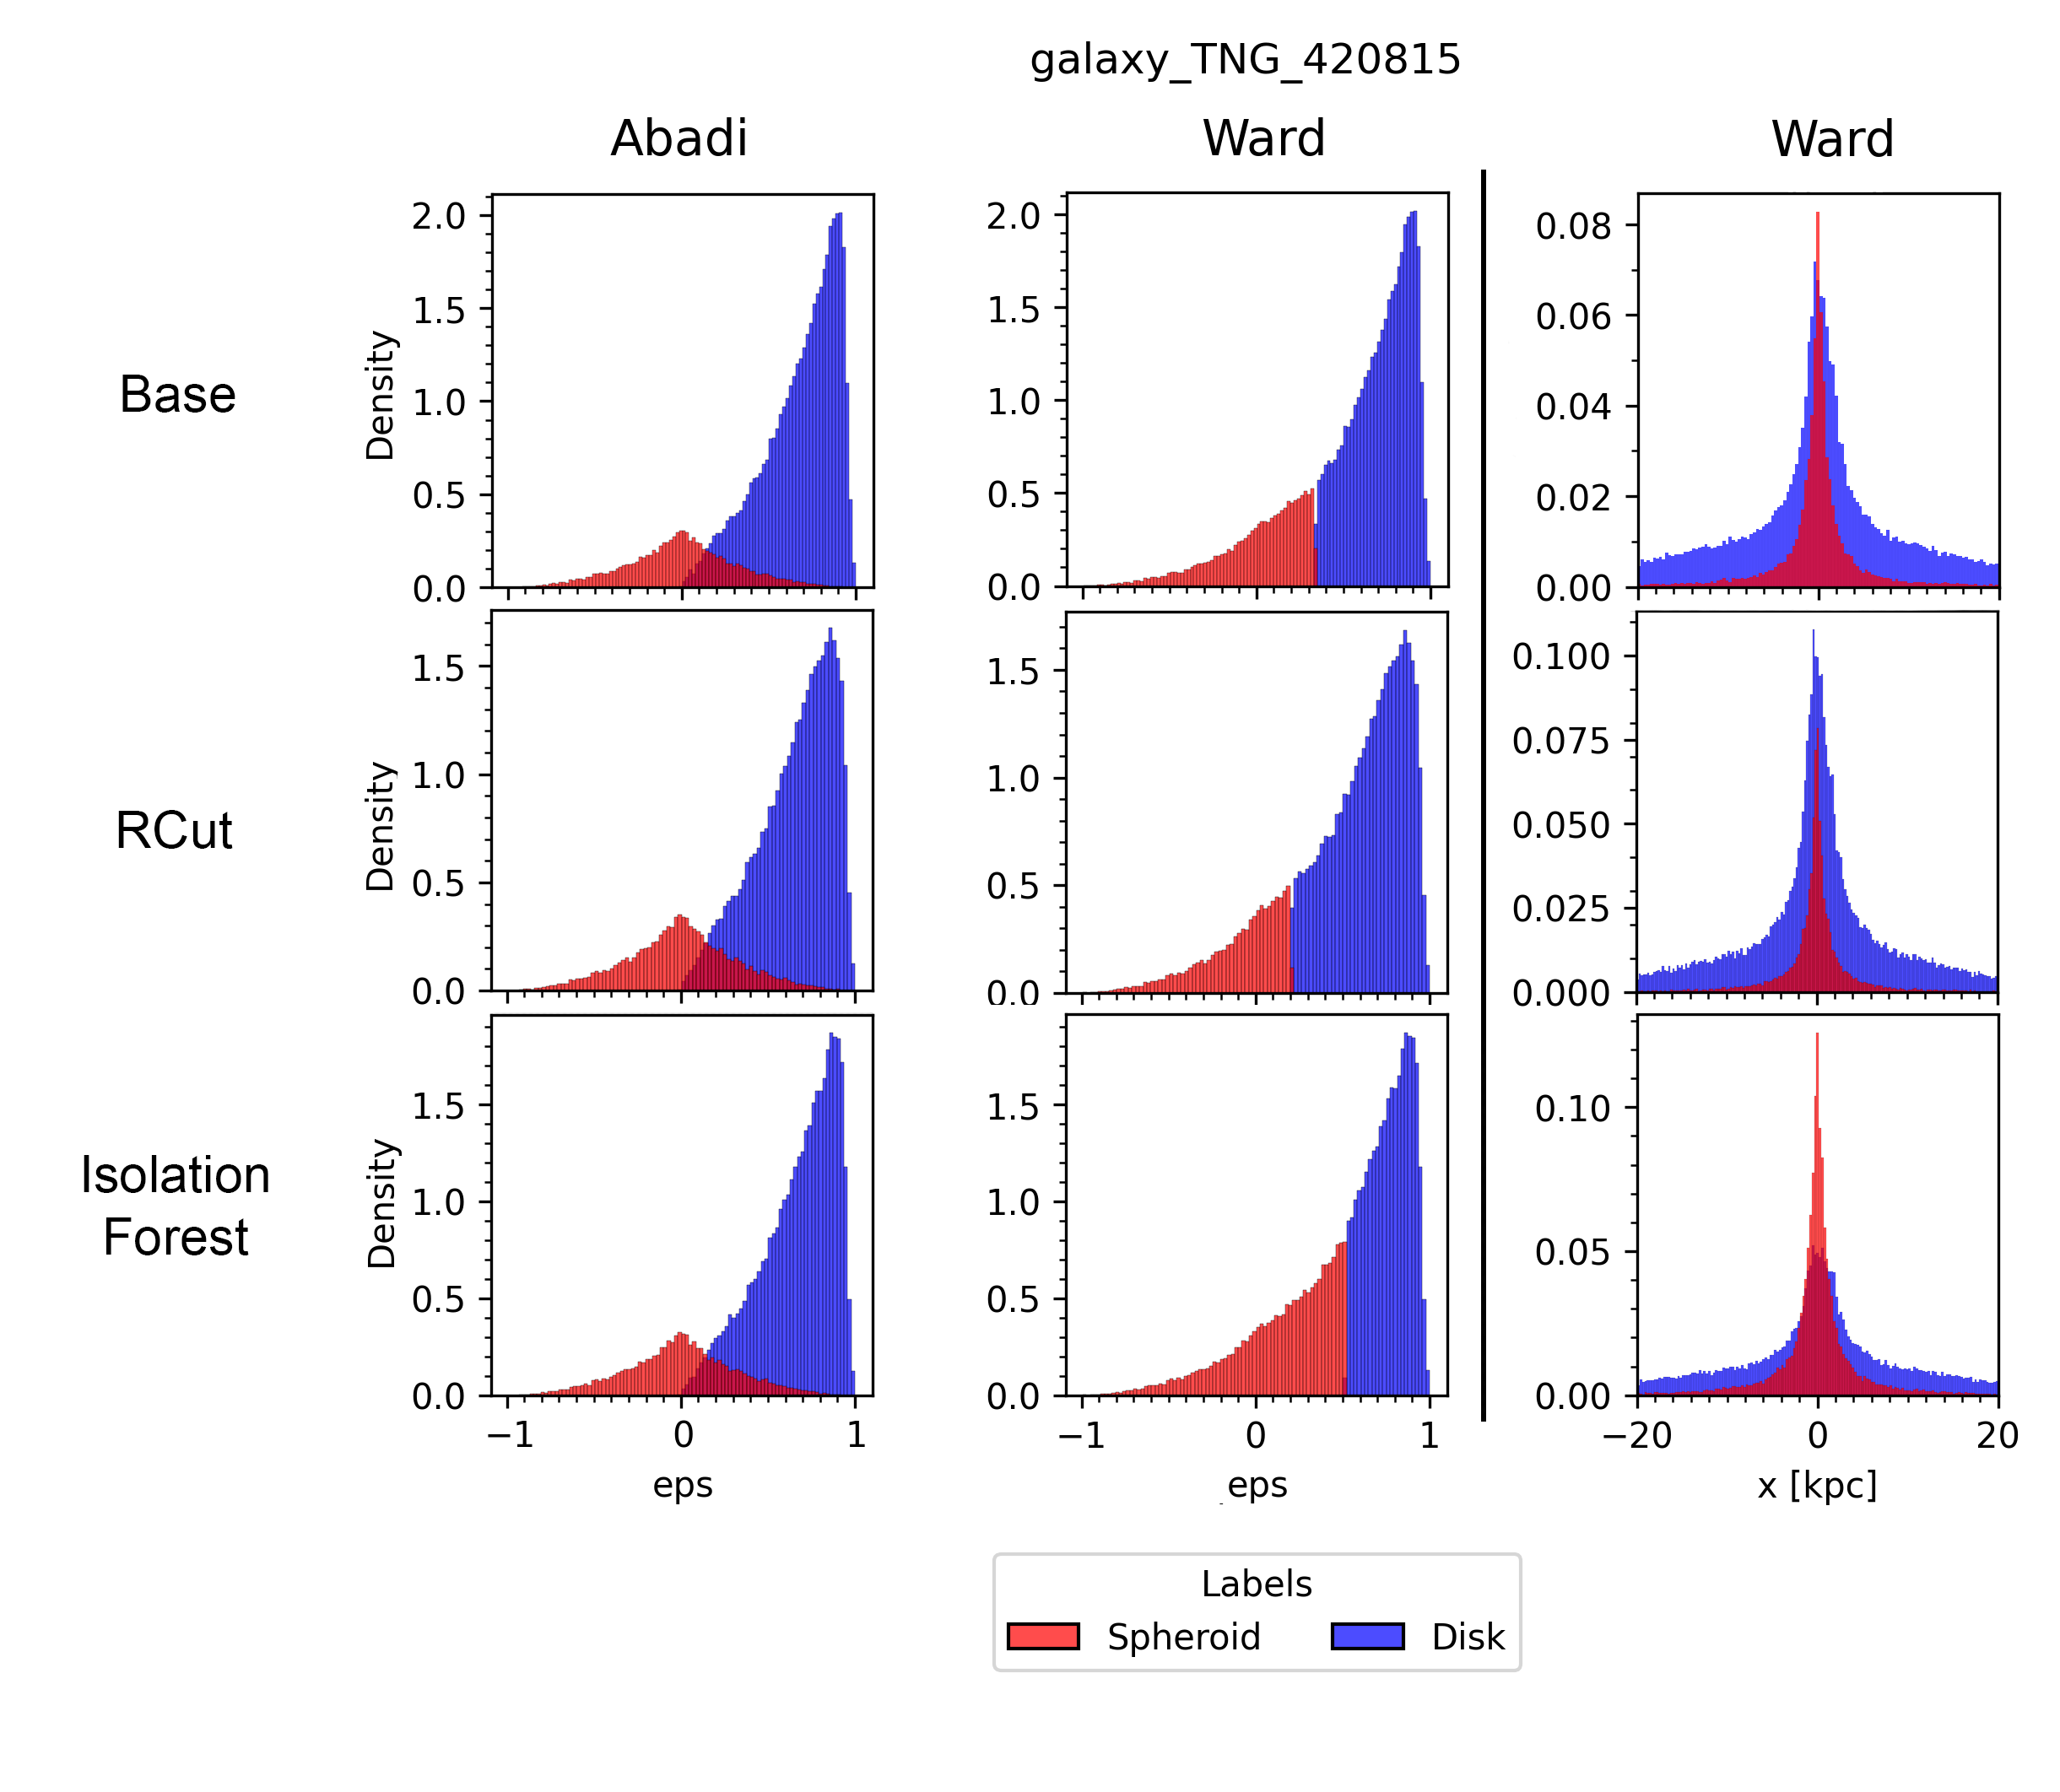
\includegraphics[width=6cm]{clustering jerarquico/figures/galaxy_TNG_420815 - abadi - base vs rcut vs isolation forest.png}
\end{center}
\column{0.5\textwidth}
\begin{center}
    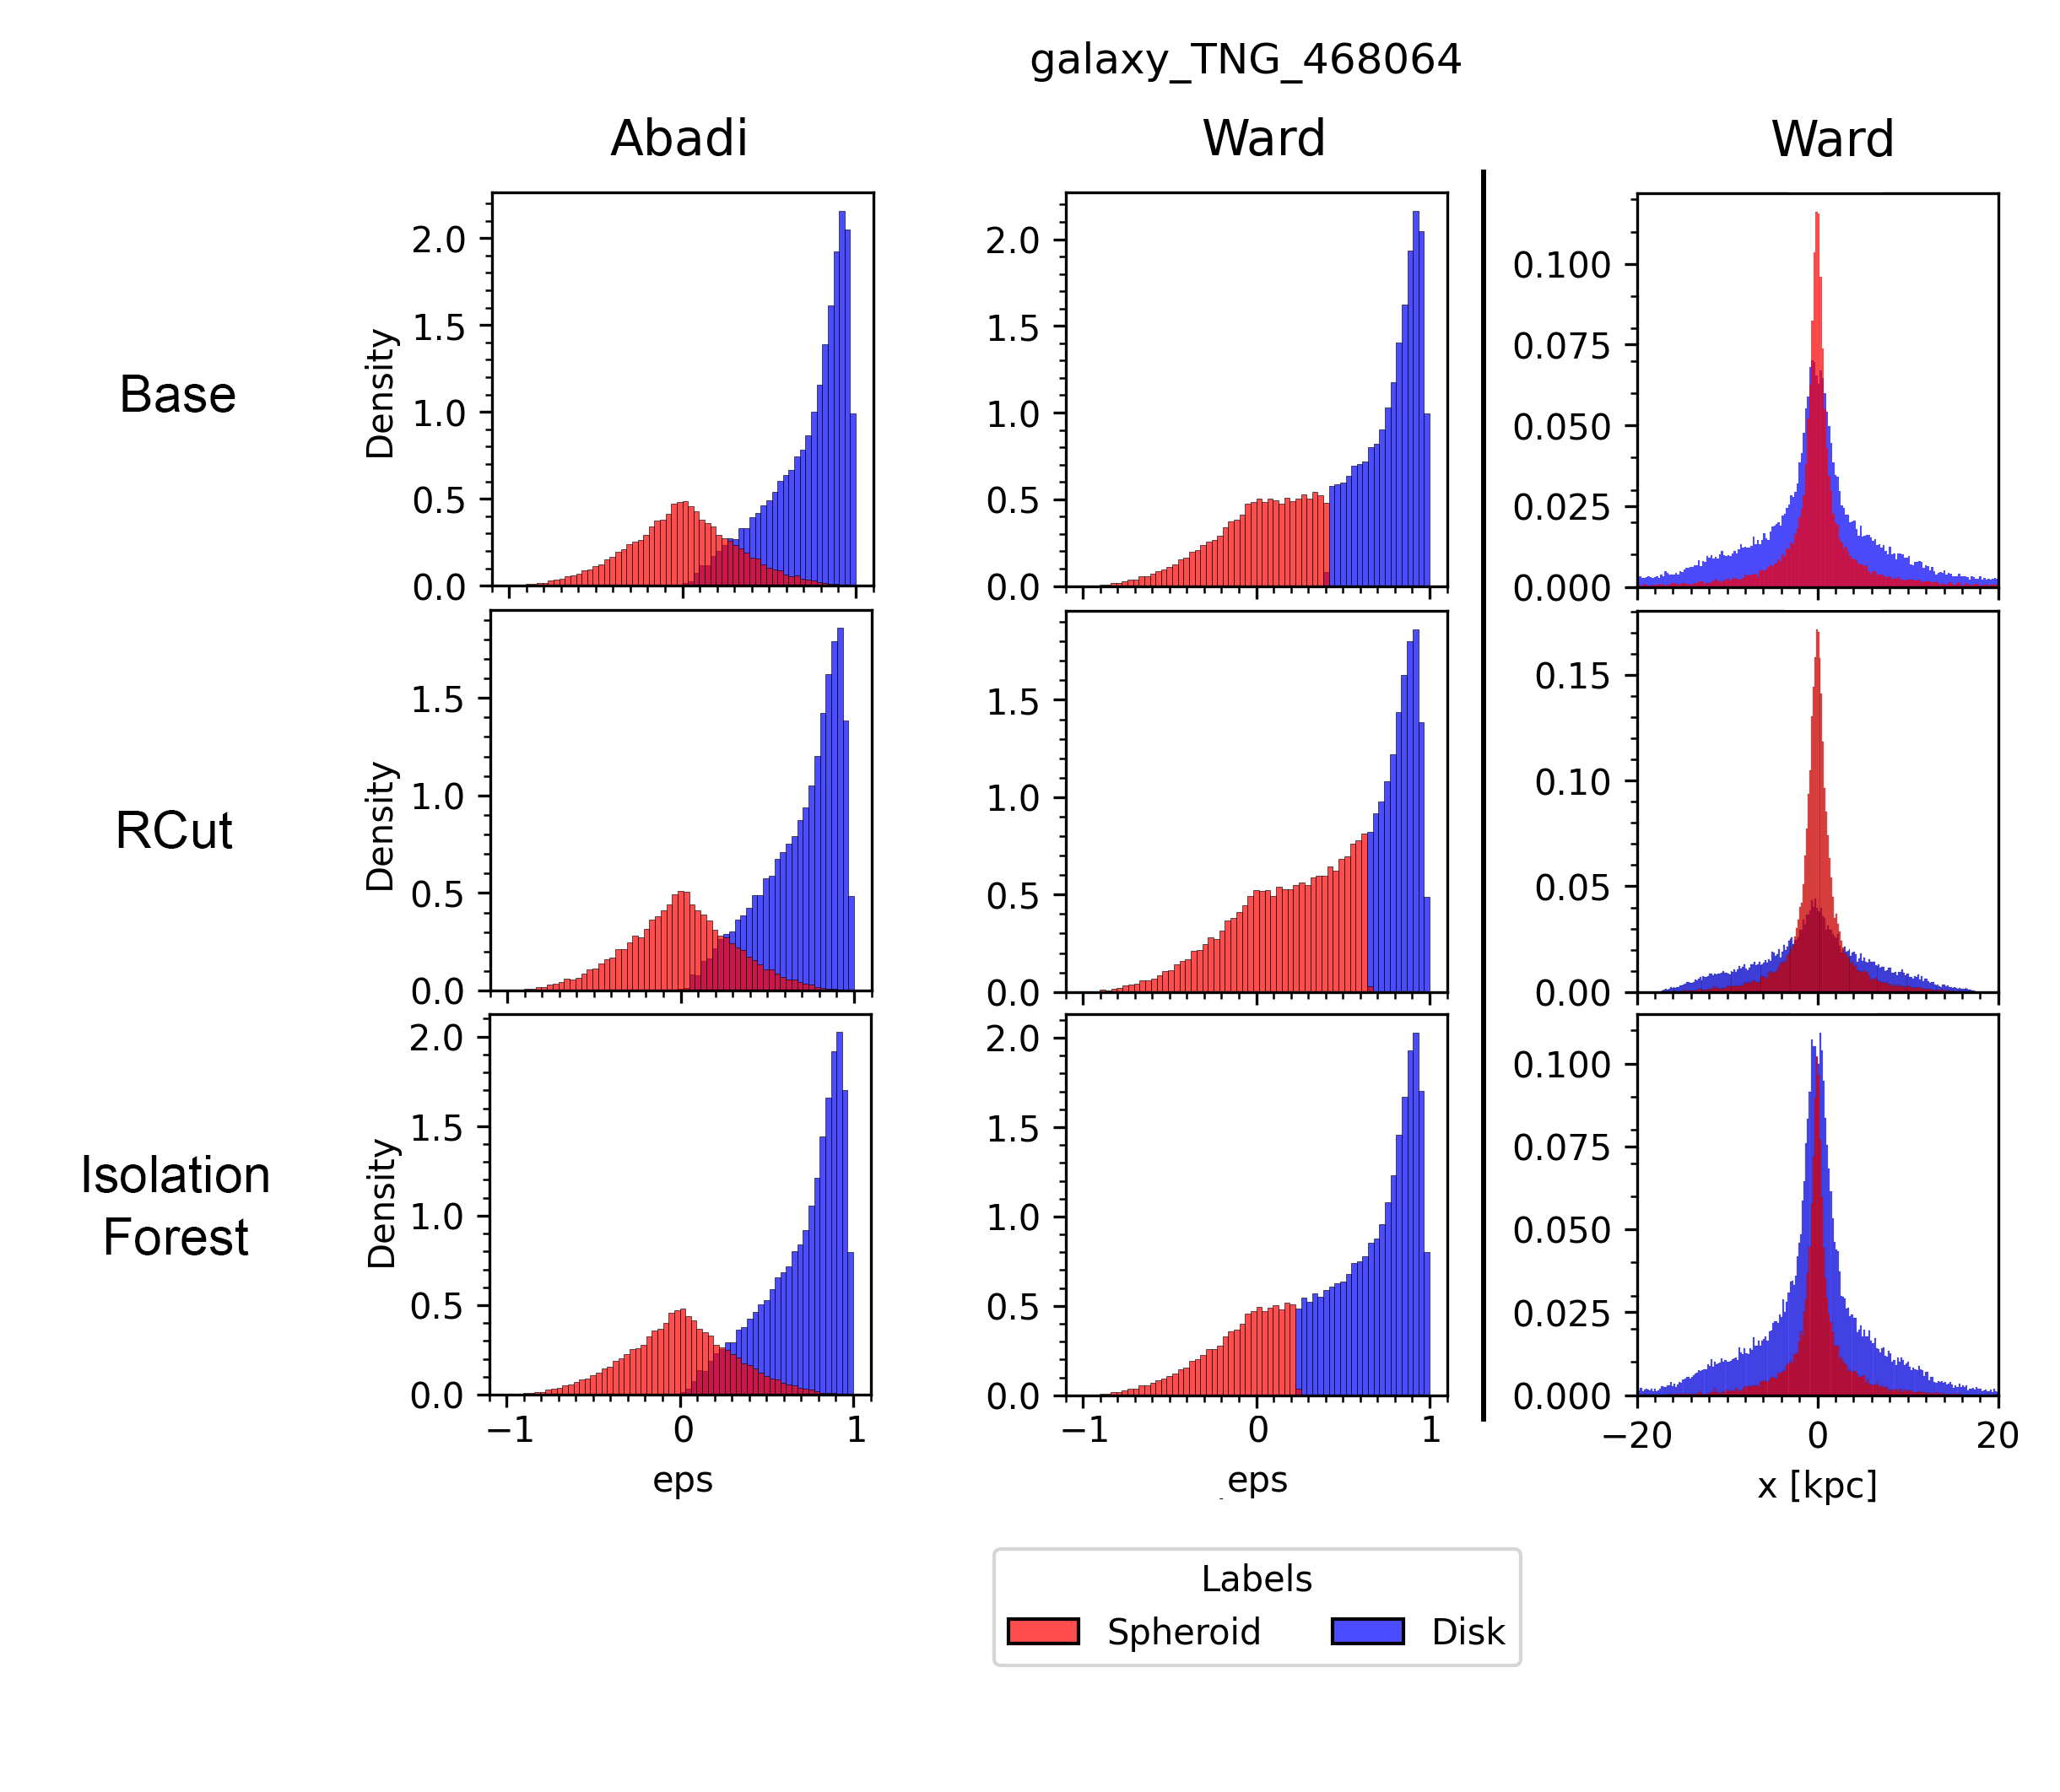
\includegraphics[width=6cm]{clustering jerarquico/figures/galaxy_TNG_468064 - abadi - base vs rcut vs isolation forest.png}
\end{center}
\end{columns}

\note{
%- cambio por que ahora el pico de densidad del esferoide bajo, entonces al minimizar la varianza cambio la linea de corte \\
%- hipotesis erronea, no podemos concluir si ayuda o no \\
- \textbf{no podemos concluir} que ayuda ni que no, para rcut ni para isolation forest \\
}

\end{frame}


\begin{frame}
\frametitle{Abadi: Eliminación de outliers}

\begin{columns}
\column{0.5\textwidth}
\begin{center}
    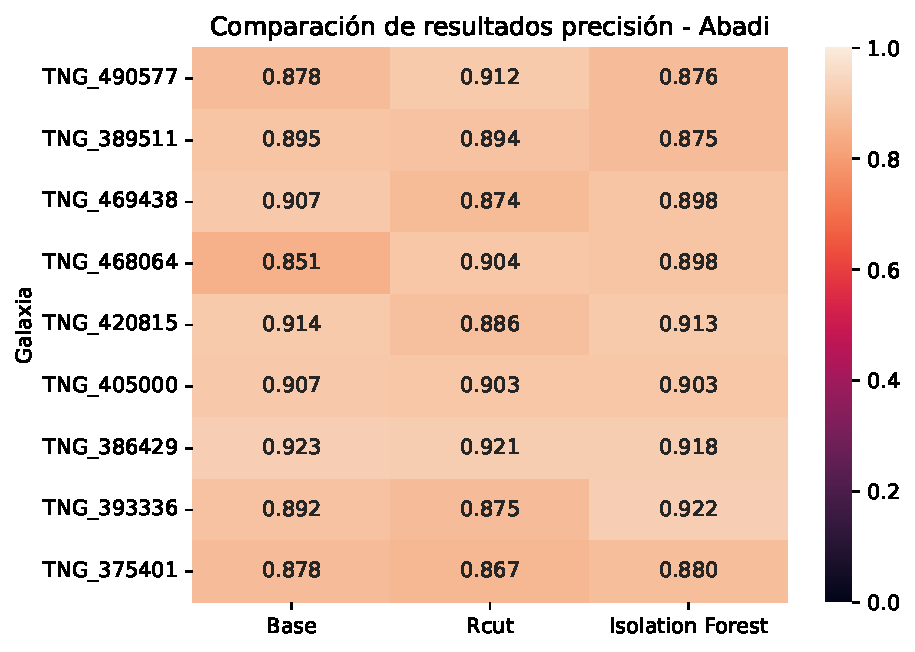
\includegraphics[width=6cm]{clustering jerarquico/figures/precision - abadi.pdf}
\end{center}
\column{0.5\textwidth}
\begin{center}
    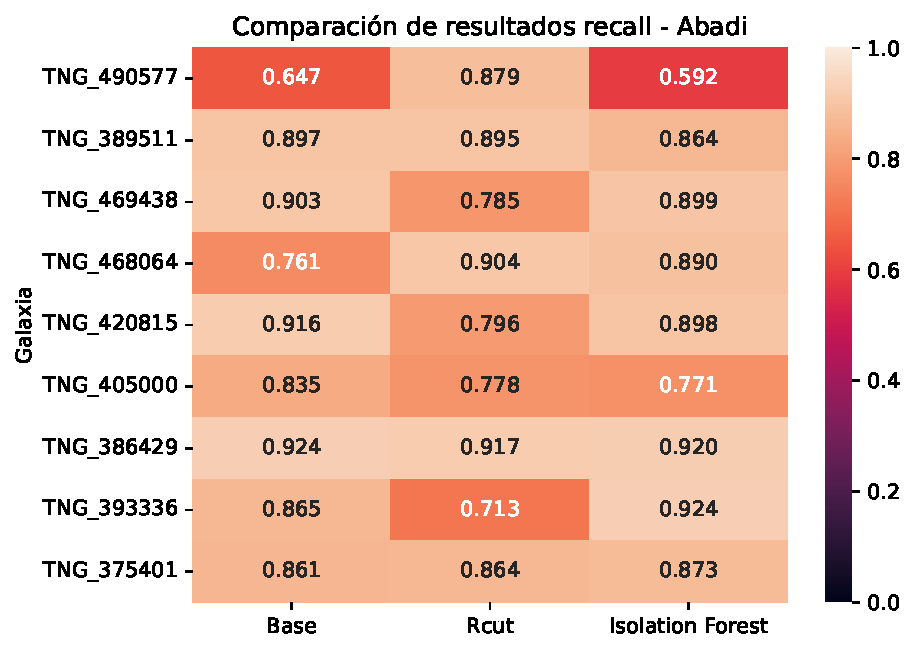
\includegraphics[width=6cm]{clustering jerarquico/figures/recall - abadi.pdf}
\end{center}
\end{columns}

\note{
- aunque en lineas generales parece dar \textbf{bien} le falta la sutileza de la \textbf{interpretacion fisica} que le da abadi a los valores \\
%- no son resultados concluyentes para decir si es bueno o no sacar outliers \\
- cj es \textbf{mas caro computacionalmente} que abadi ($O(n^2)$), incluso si da mejor no nos sirve como alternativa del dia a dia
}

\end{frame}


% cj es mas caro que abadi, incluso si da mejor no nos sirve como alternativa del dia a dia
% Como nota final, podemos concluir que el \gls{HC} se comporta, como mucho, de forma similar a Abadi al buscar 2 clusters, pero como éste es más caro en memoria y computacionalmente (ya que calcula una matriz de distancia, por lo que estamos hablando de magnitudes de $O(n^2)$ para ambos), al final del día el algoritmo de Abadi sigue siendo la mejor alternativa.



\begin{frame}
\frametitle{AGMM: Detección de $=>$2 componentes}

\begin{center}
    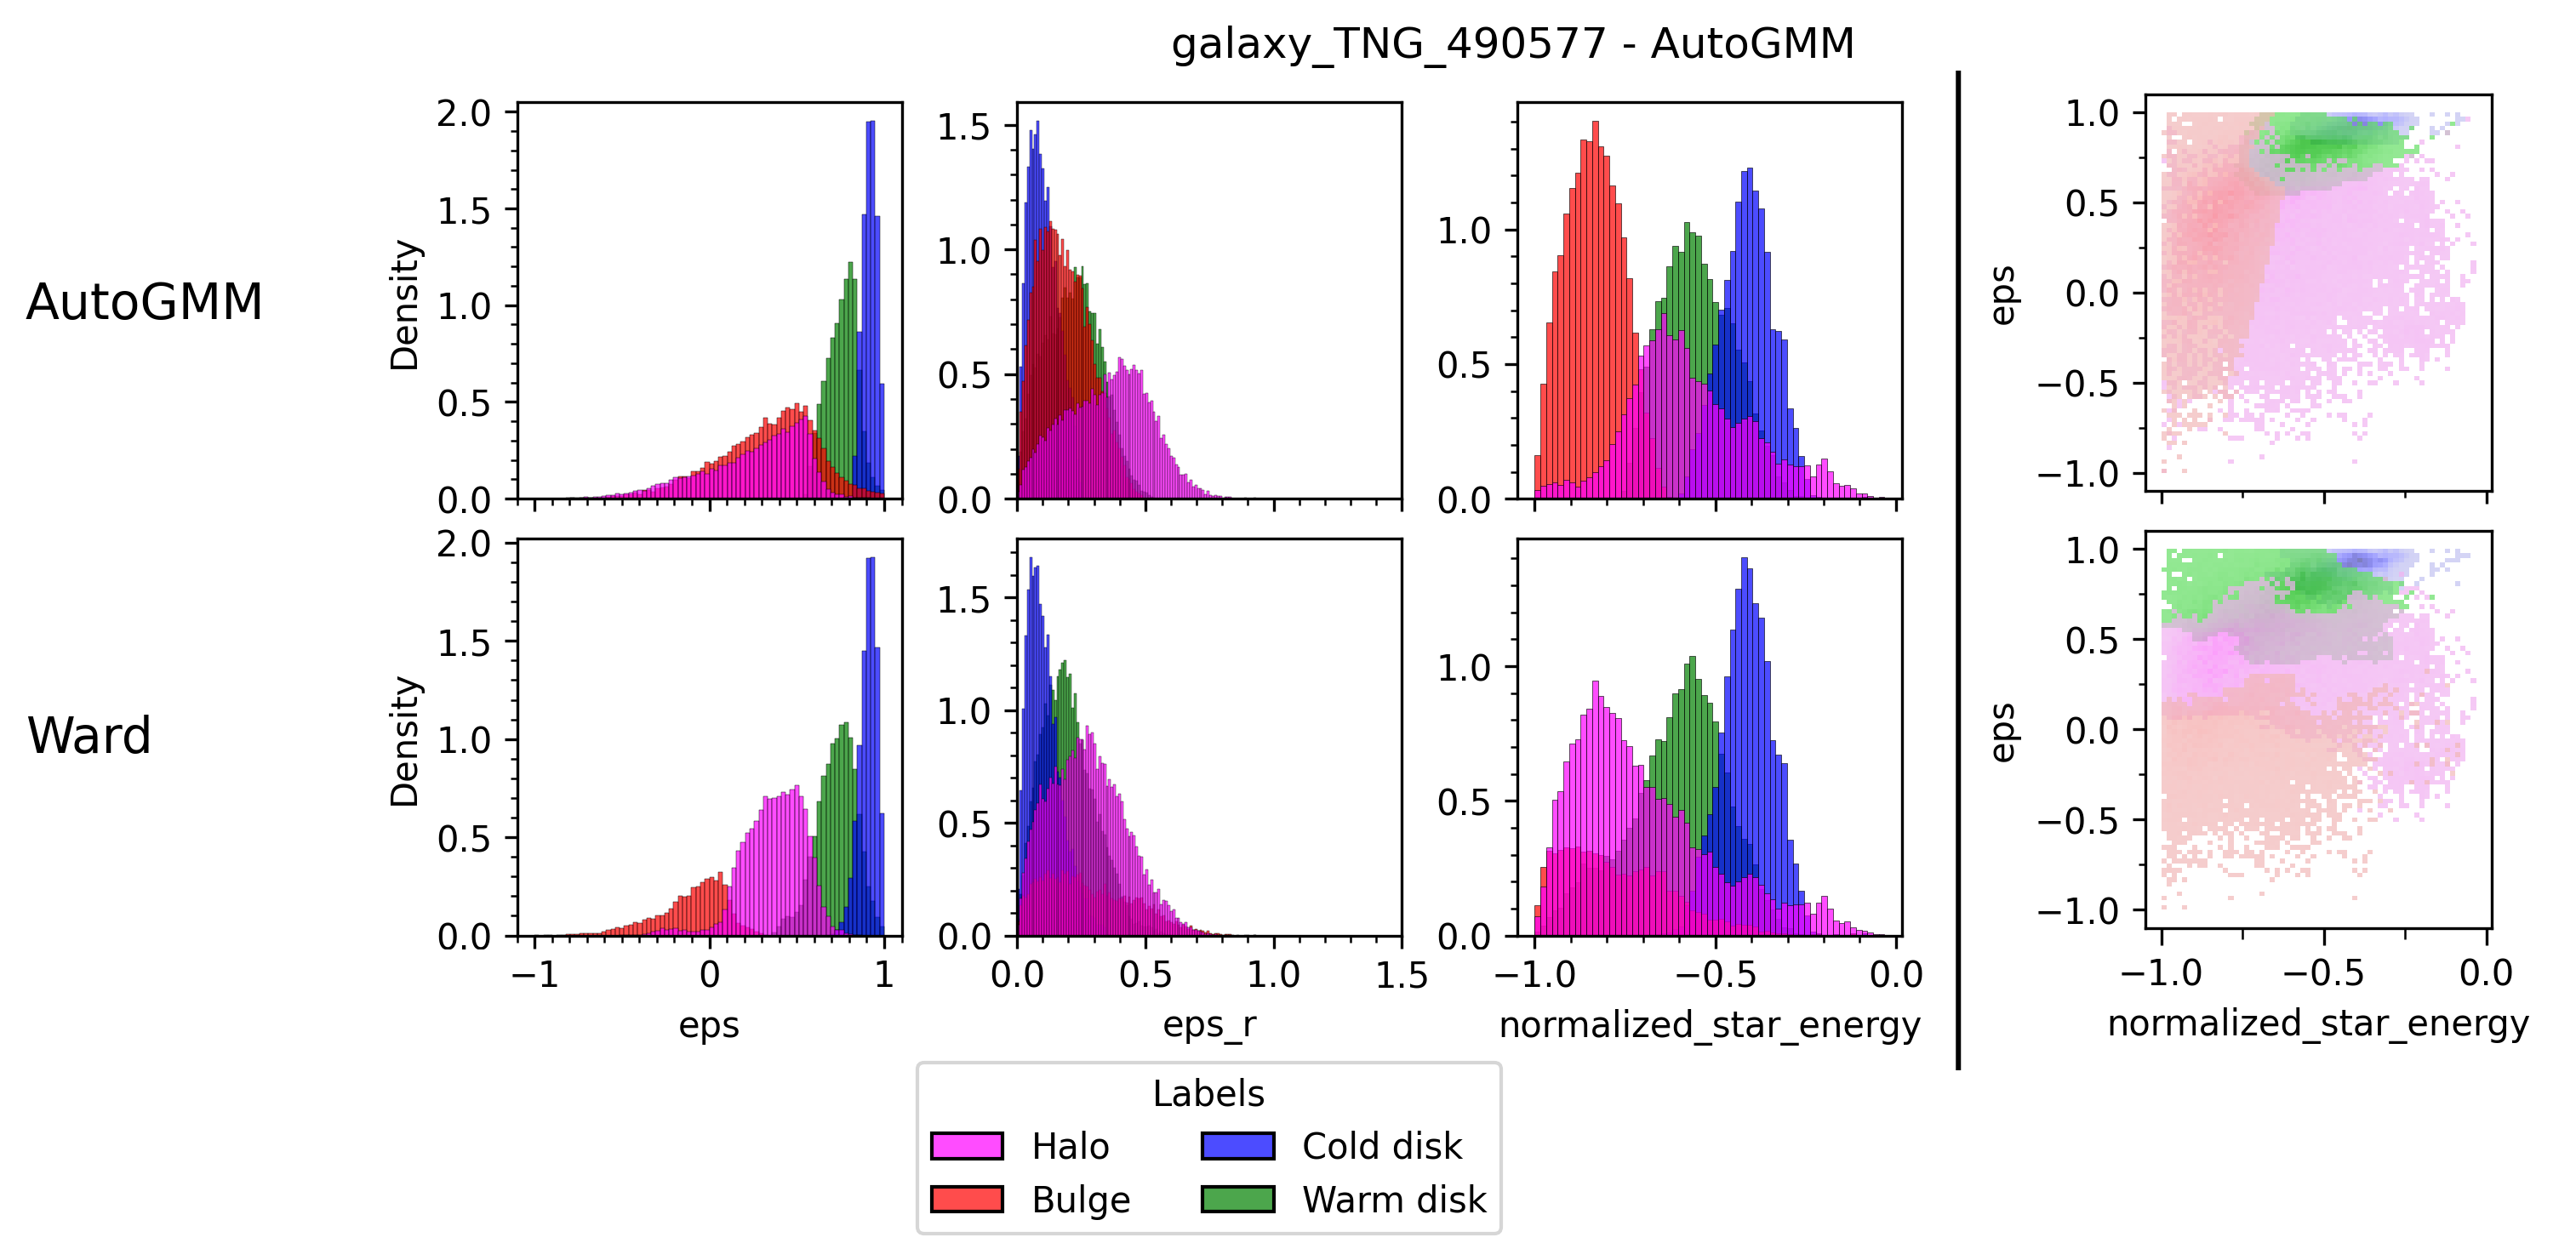
\includegraphics[width=12cm]{clustering jerarquico/figures/AGMM - galaxy_TNG_490577 - circ histogram.png}
\end{center}

\note{
%- Si nos dio mal los linkages antes seria raro que nos de bien ahora, por eso partimos directamente usando Ward \\
%- Idea jerarquica de las componentes. Al comparar contra Abadi antes, esperariamos que ahora, al buscar mas componentes, encontremos el \textbf{Disco fino y grueso dentro de lo que era el Disco}. No es un problema para el Disco, pero lo es con el Esferoide \\
%- Explicar porque se \textbf{solapa halo y bulge en AGMM, pero no en HC}: Como \textbf{Esferoide} es soportado por dispercion de velocidades, sus \textbf{particulas tienen gran variacion en eps}. Esto tambien es verdad para sus \textbf{subcomponentes}, Halo y Bulge, por lo que se ven solapadas en AGMM. \\
- \textbf{Halo y Bulge se ven separados en eps en lugar de solapados}\\
- Como el linkage \textbf{Ward} busca \textbf{minimizar la varianza de cada cluster}, esto se traduce en buscar que los \textbf{clusters estén lo más separados entre ellos}, lo cual va en directa contraposición con la \textbf{naturaleza de las componentes mencionadas} (incluso si esta bien para clusterizacion en general)
}



\end{frame}

\iflong
\begin{frame}
\frametitle{AGMM: Detección de $=>$2 componentes}

\begin{center}
    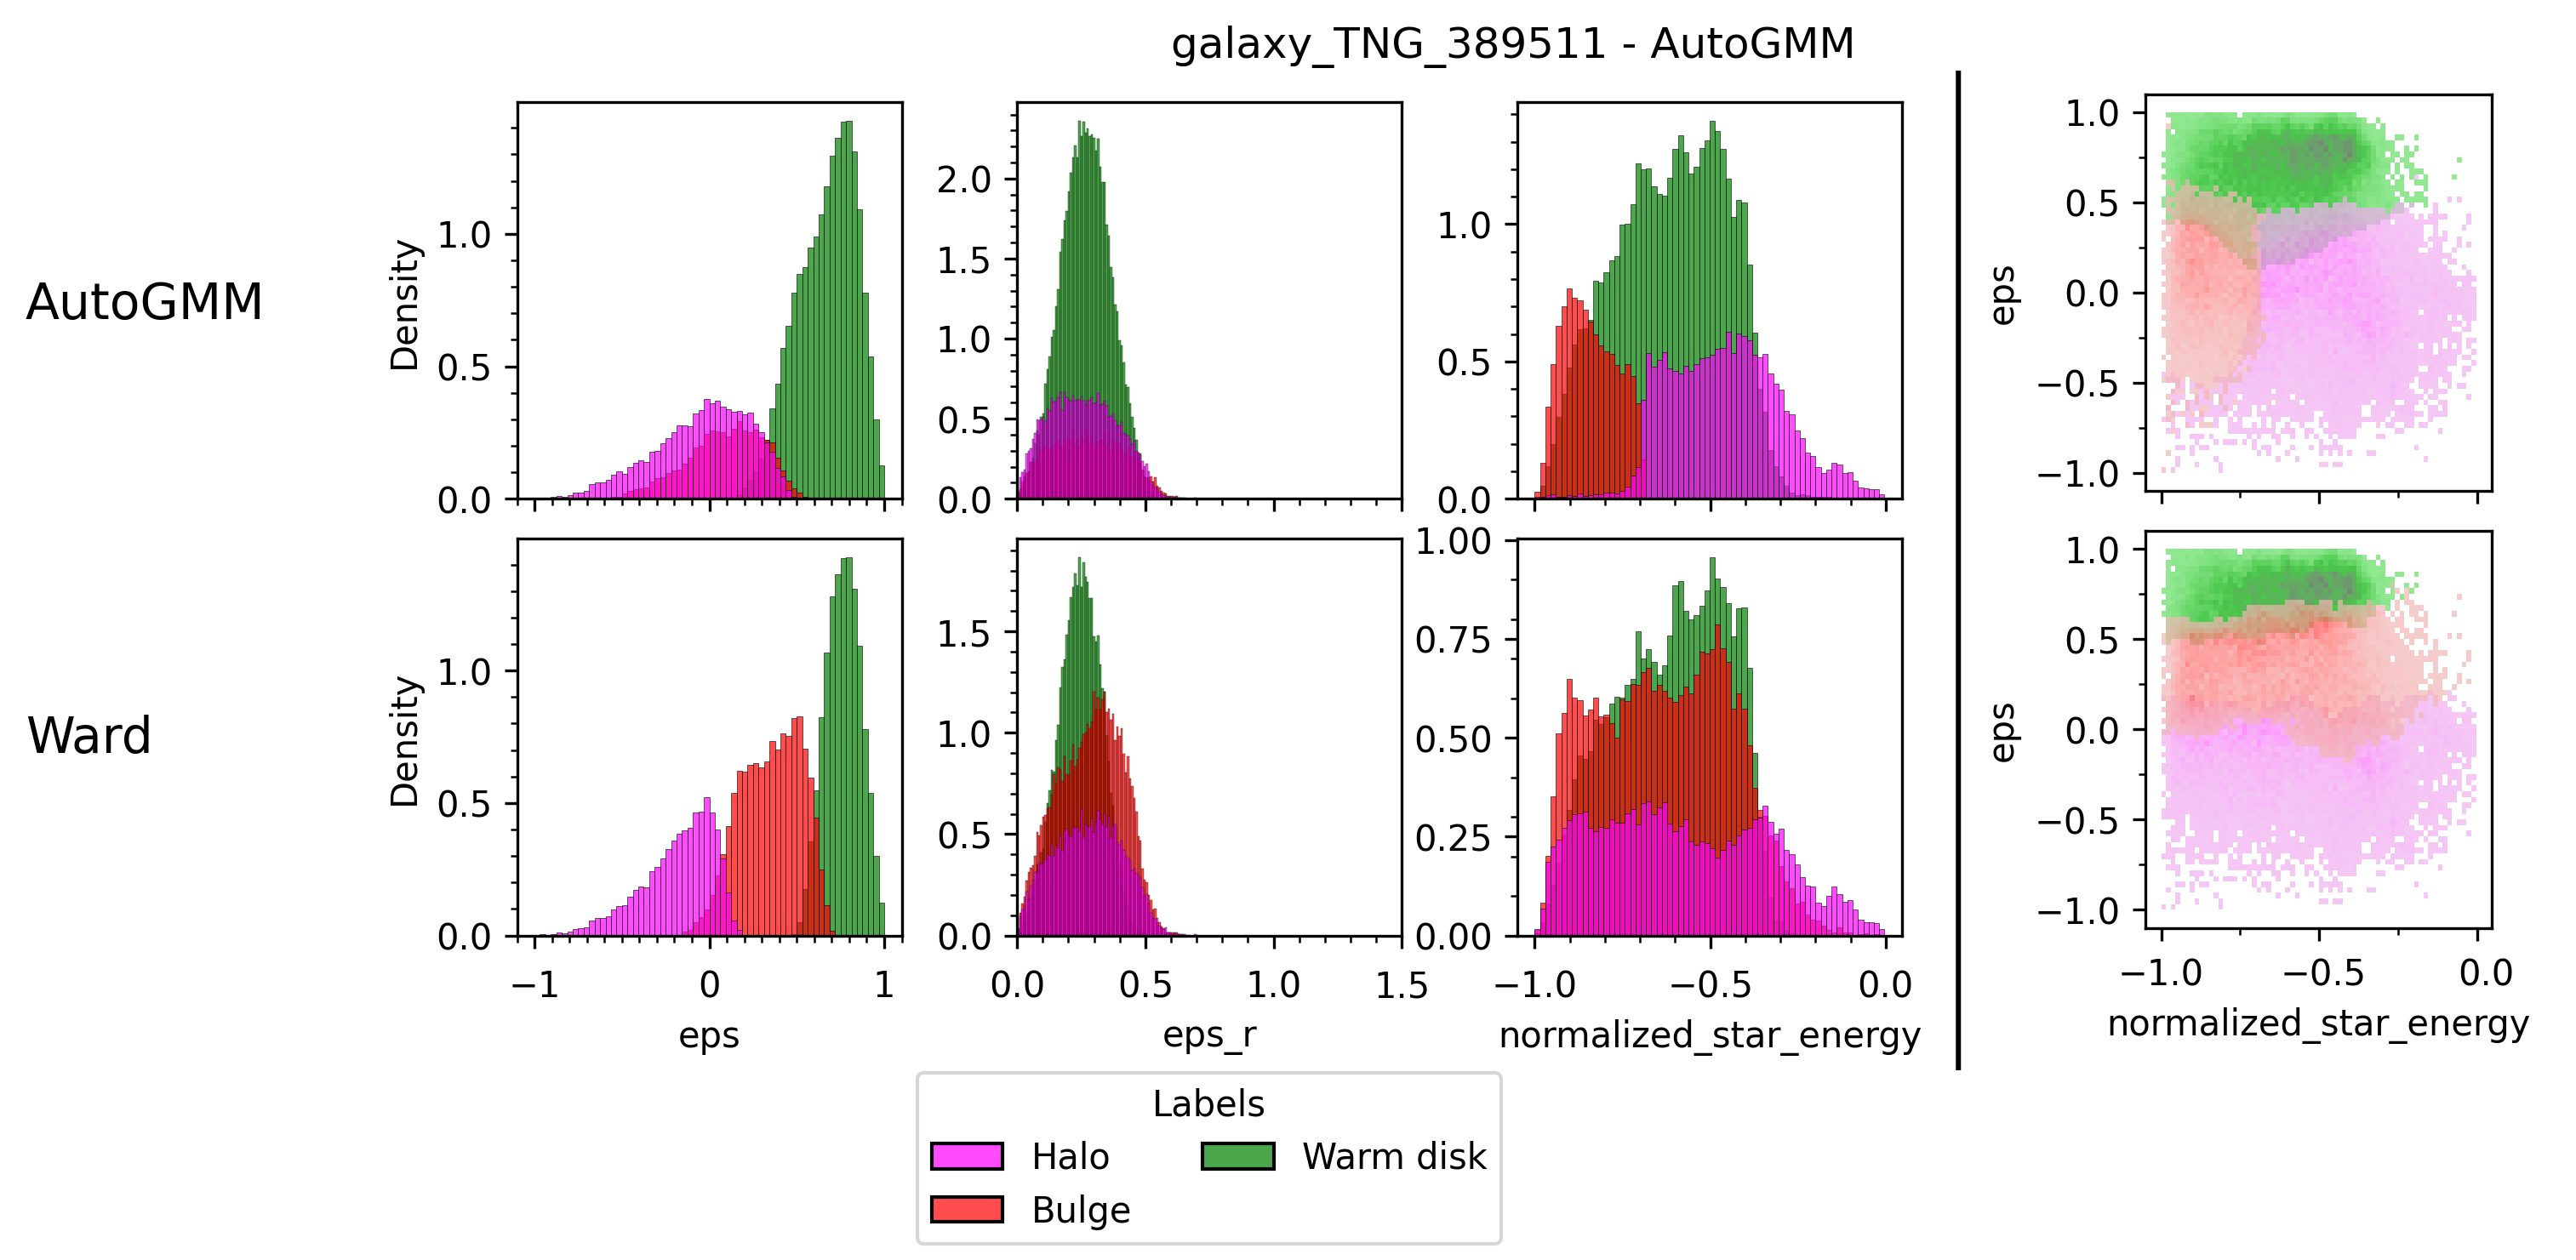
\includegraphics[width=12cm]{clustering jerarquico/figures/AGMM - galaxy_TNG_389511 - circ histogram.png}
\end{center}

\note{
- \textbf{$eps$ no es una buena feature para identificar Halo y Bulge}. La \textbf{siguiente mejor es $normalized\_star\_energy$} segun el orden de relevancia en el area. Y podemos confirmar su importancia al mirar como se dividen estas en AGMM. Pero el Warm disk solapa ahi y le complica a Ward usar la feature como corresponde para identificar componentes. Corte unidimensional en el scatterplot.\\
%- Como las componentes del Disco son soportadas por rotación, esto significa que predomina el movimiento ordenado, por lo que ambos discos tienen sus componentes mas acotadas en eps y son mas faciles de identificar por CJ (diapo anterior). \\
}

\end{frame}
\fi

\begin{frame}
\frametitle{AGMM: Detección de $=>$2 componentes}

\begin{columns}
\column{0.5\textwidth}
\begin{center}
    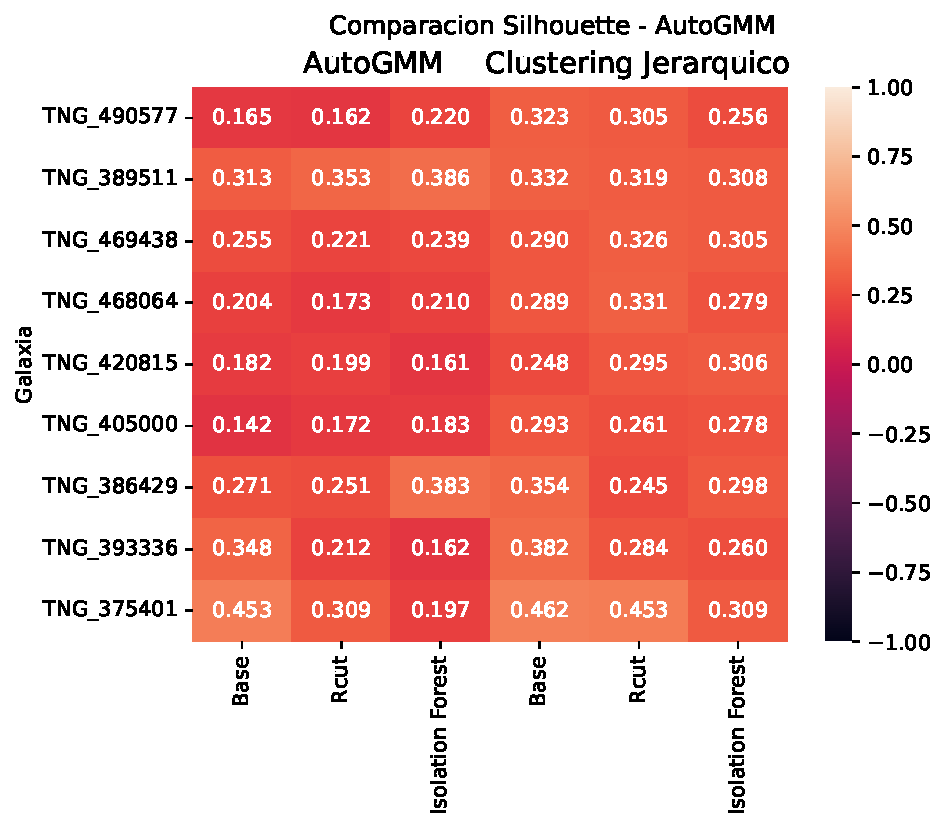
\includegraphics[width=6cm]{clustering jerarquico/figures/silhouette - agmm.pdf}
\end{center}
\column{0.5\textwidth}
\begin{center}
    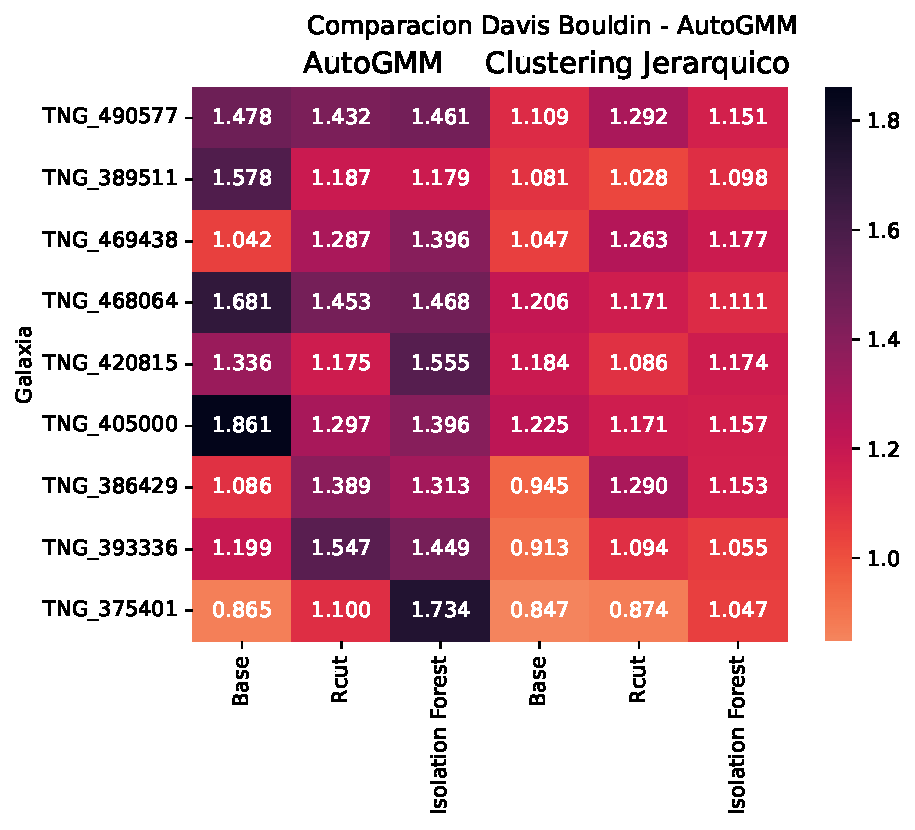
\includegraphics[width=6cm]{clustering jerarquico/figures/davis bouldin - agmm.pdf}
\end{center}
\end{columns}

\note{
- Las metricas internas dicen que ward da mejor que agmm, pero \textbf{esta mal} \\
- Distinción entre lo que es \textbf{más correcto} a la hora de \textbf{buscar clusters abstractos} contra buscar componentes de una galaxia \\
- Estas métricas son calculadas a partir del \textbf{concepto ideal abstracto de cluster}, el cual se basa en que éstos sean compactos, separados espacialmente están entre ellos, y que exista ``continuidad'' en cada uno. \\
}

\end{frame}


\iflong
\begin{frame}
\frametitle{AGMM: Detección de $=>$2 componentes}

\begin{columns}
\column{0.5\textwidth}
\begin{center}
    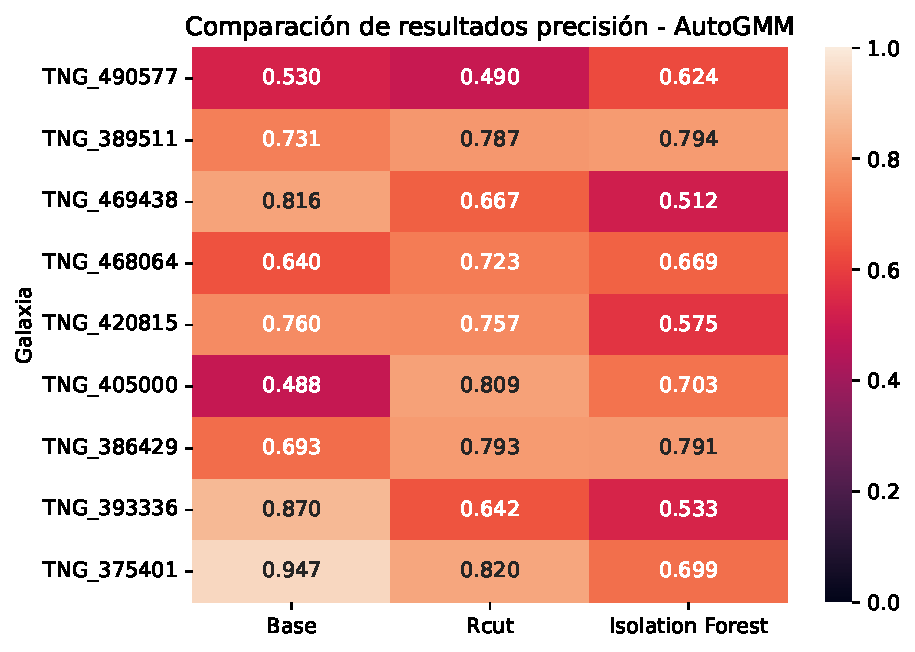
\includegraphics[width=6cm]{clustering jerarquico/figures/precision - agmm.pdf}
\end{center}
\column{0.5\textwidth}
\begin{center}
    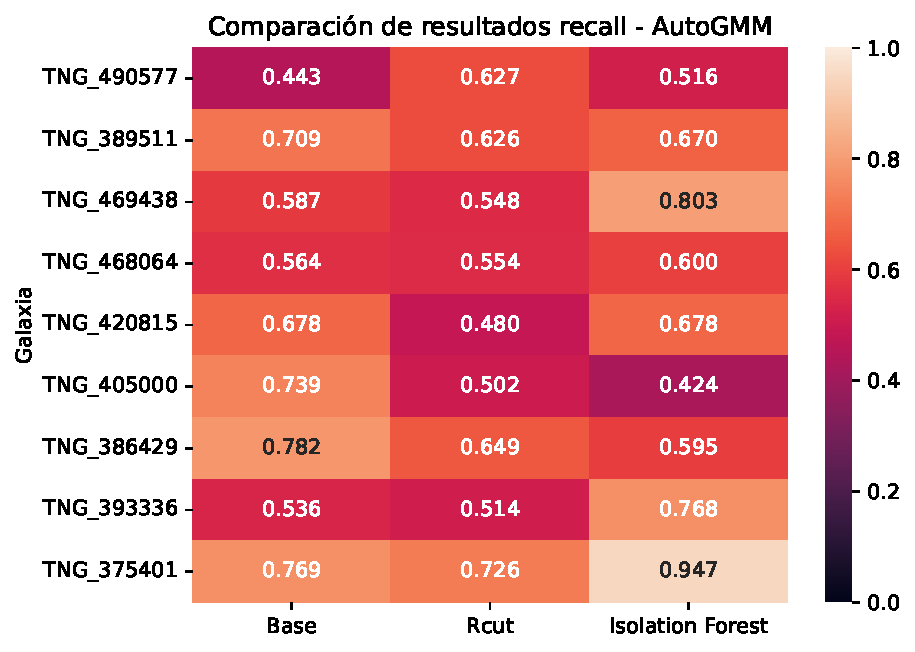
\includegraphics[width=6cm]{clustering jerarquico/figures/recall - agmm.pdf}
\end{center}
\end{columns}

\note{
- presicion y recall promedio dan mas de 0.5 pero no mucho mas, por lo que no son muy buenas \\
%- las soluciones del método jerárquico con más clusters son particiones de las soluciones con menos clusters, por lo cual solo pueden aumentar el error al aumentar la cantidad de clusters a buscar (mas clusters a buscar va a empeorar el error)
}

\end{frame}
\fi



\begin{frame}
\frametitle{AGMM: Eliminación de outliers}

\begin{center}
    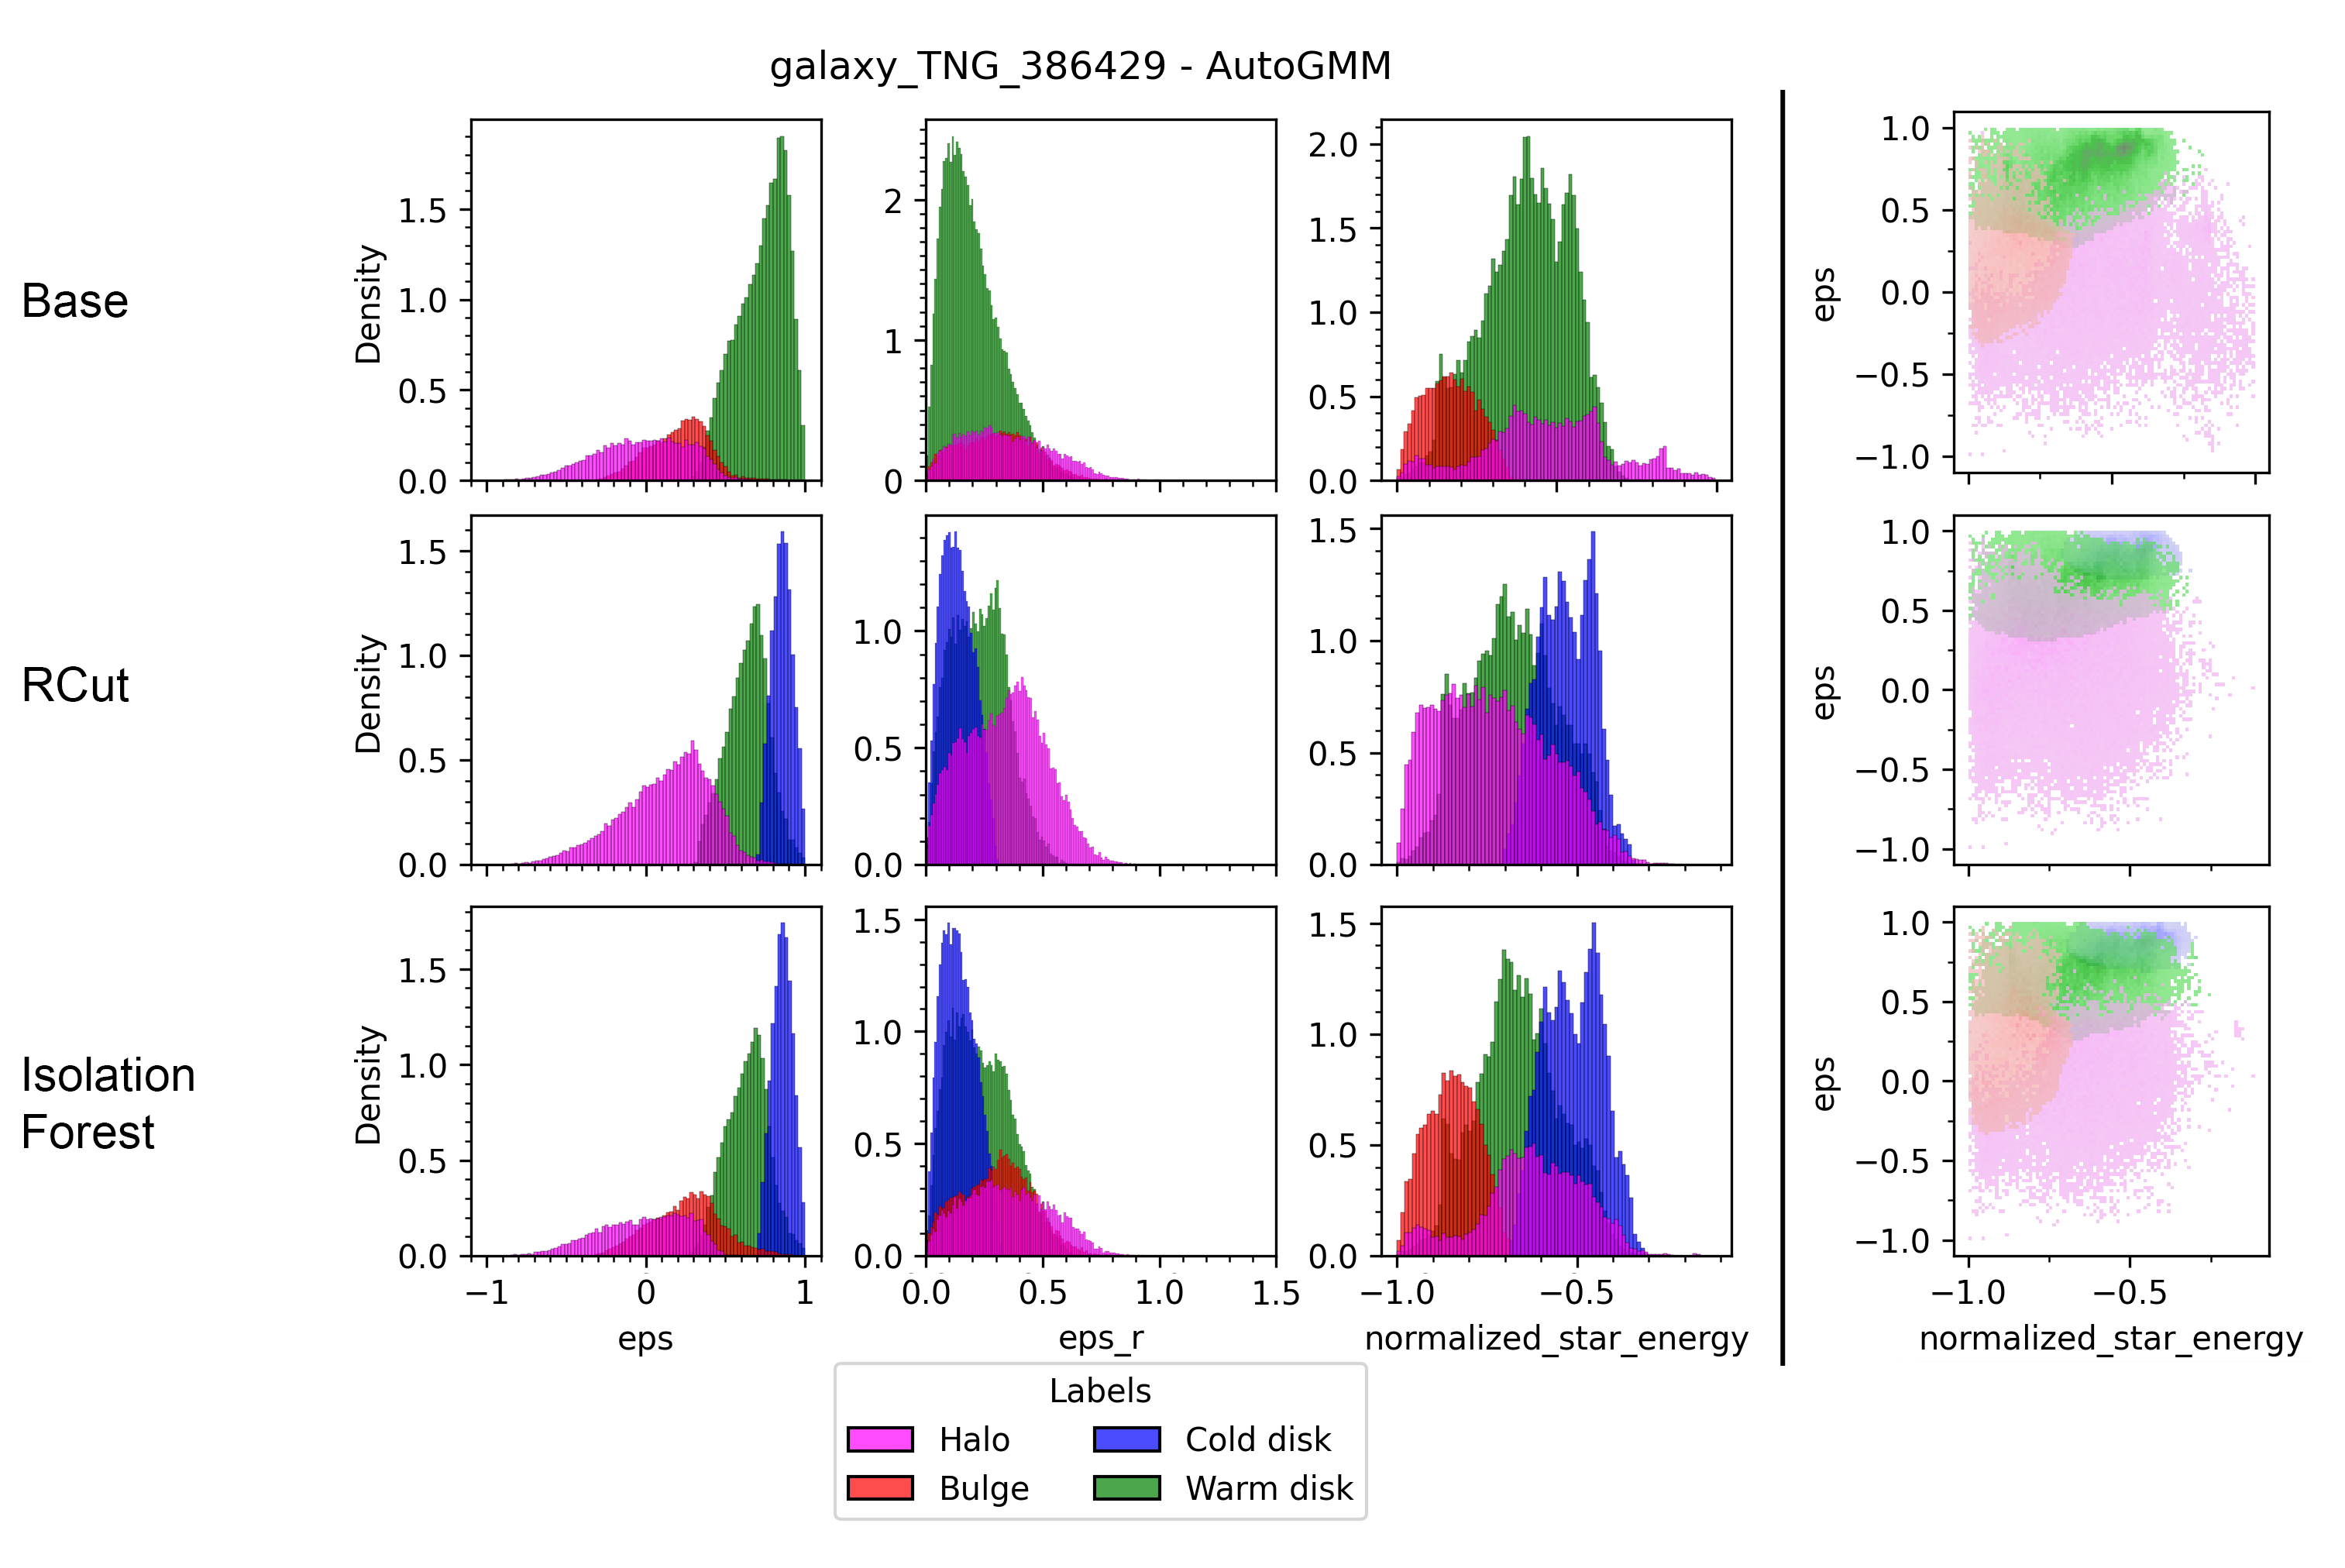
\includegraphics[width=12cm]{clustering jerarquico/figures/AGMM - different components found.png}
\end{center}

\note{
- remover outliers te puede cambiar la \textbf{cantidad de clusters} encontrados por como funciona agmm, lo cual dificulta la comparacion \\
}

\end{frame}


\begin{frame}
\frametitle{AGMM: Eliminación de outliers}
% - igualmente, con los datos que tenemos no podemos decir que sirva
\begin{center}
    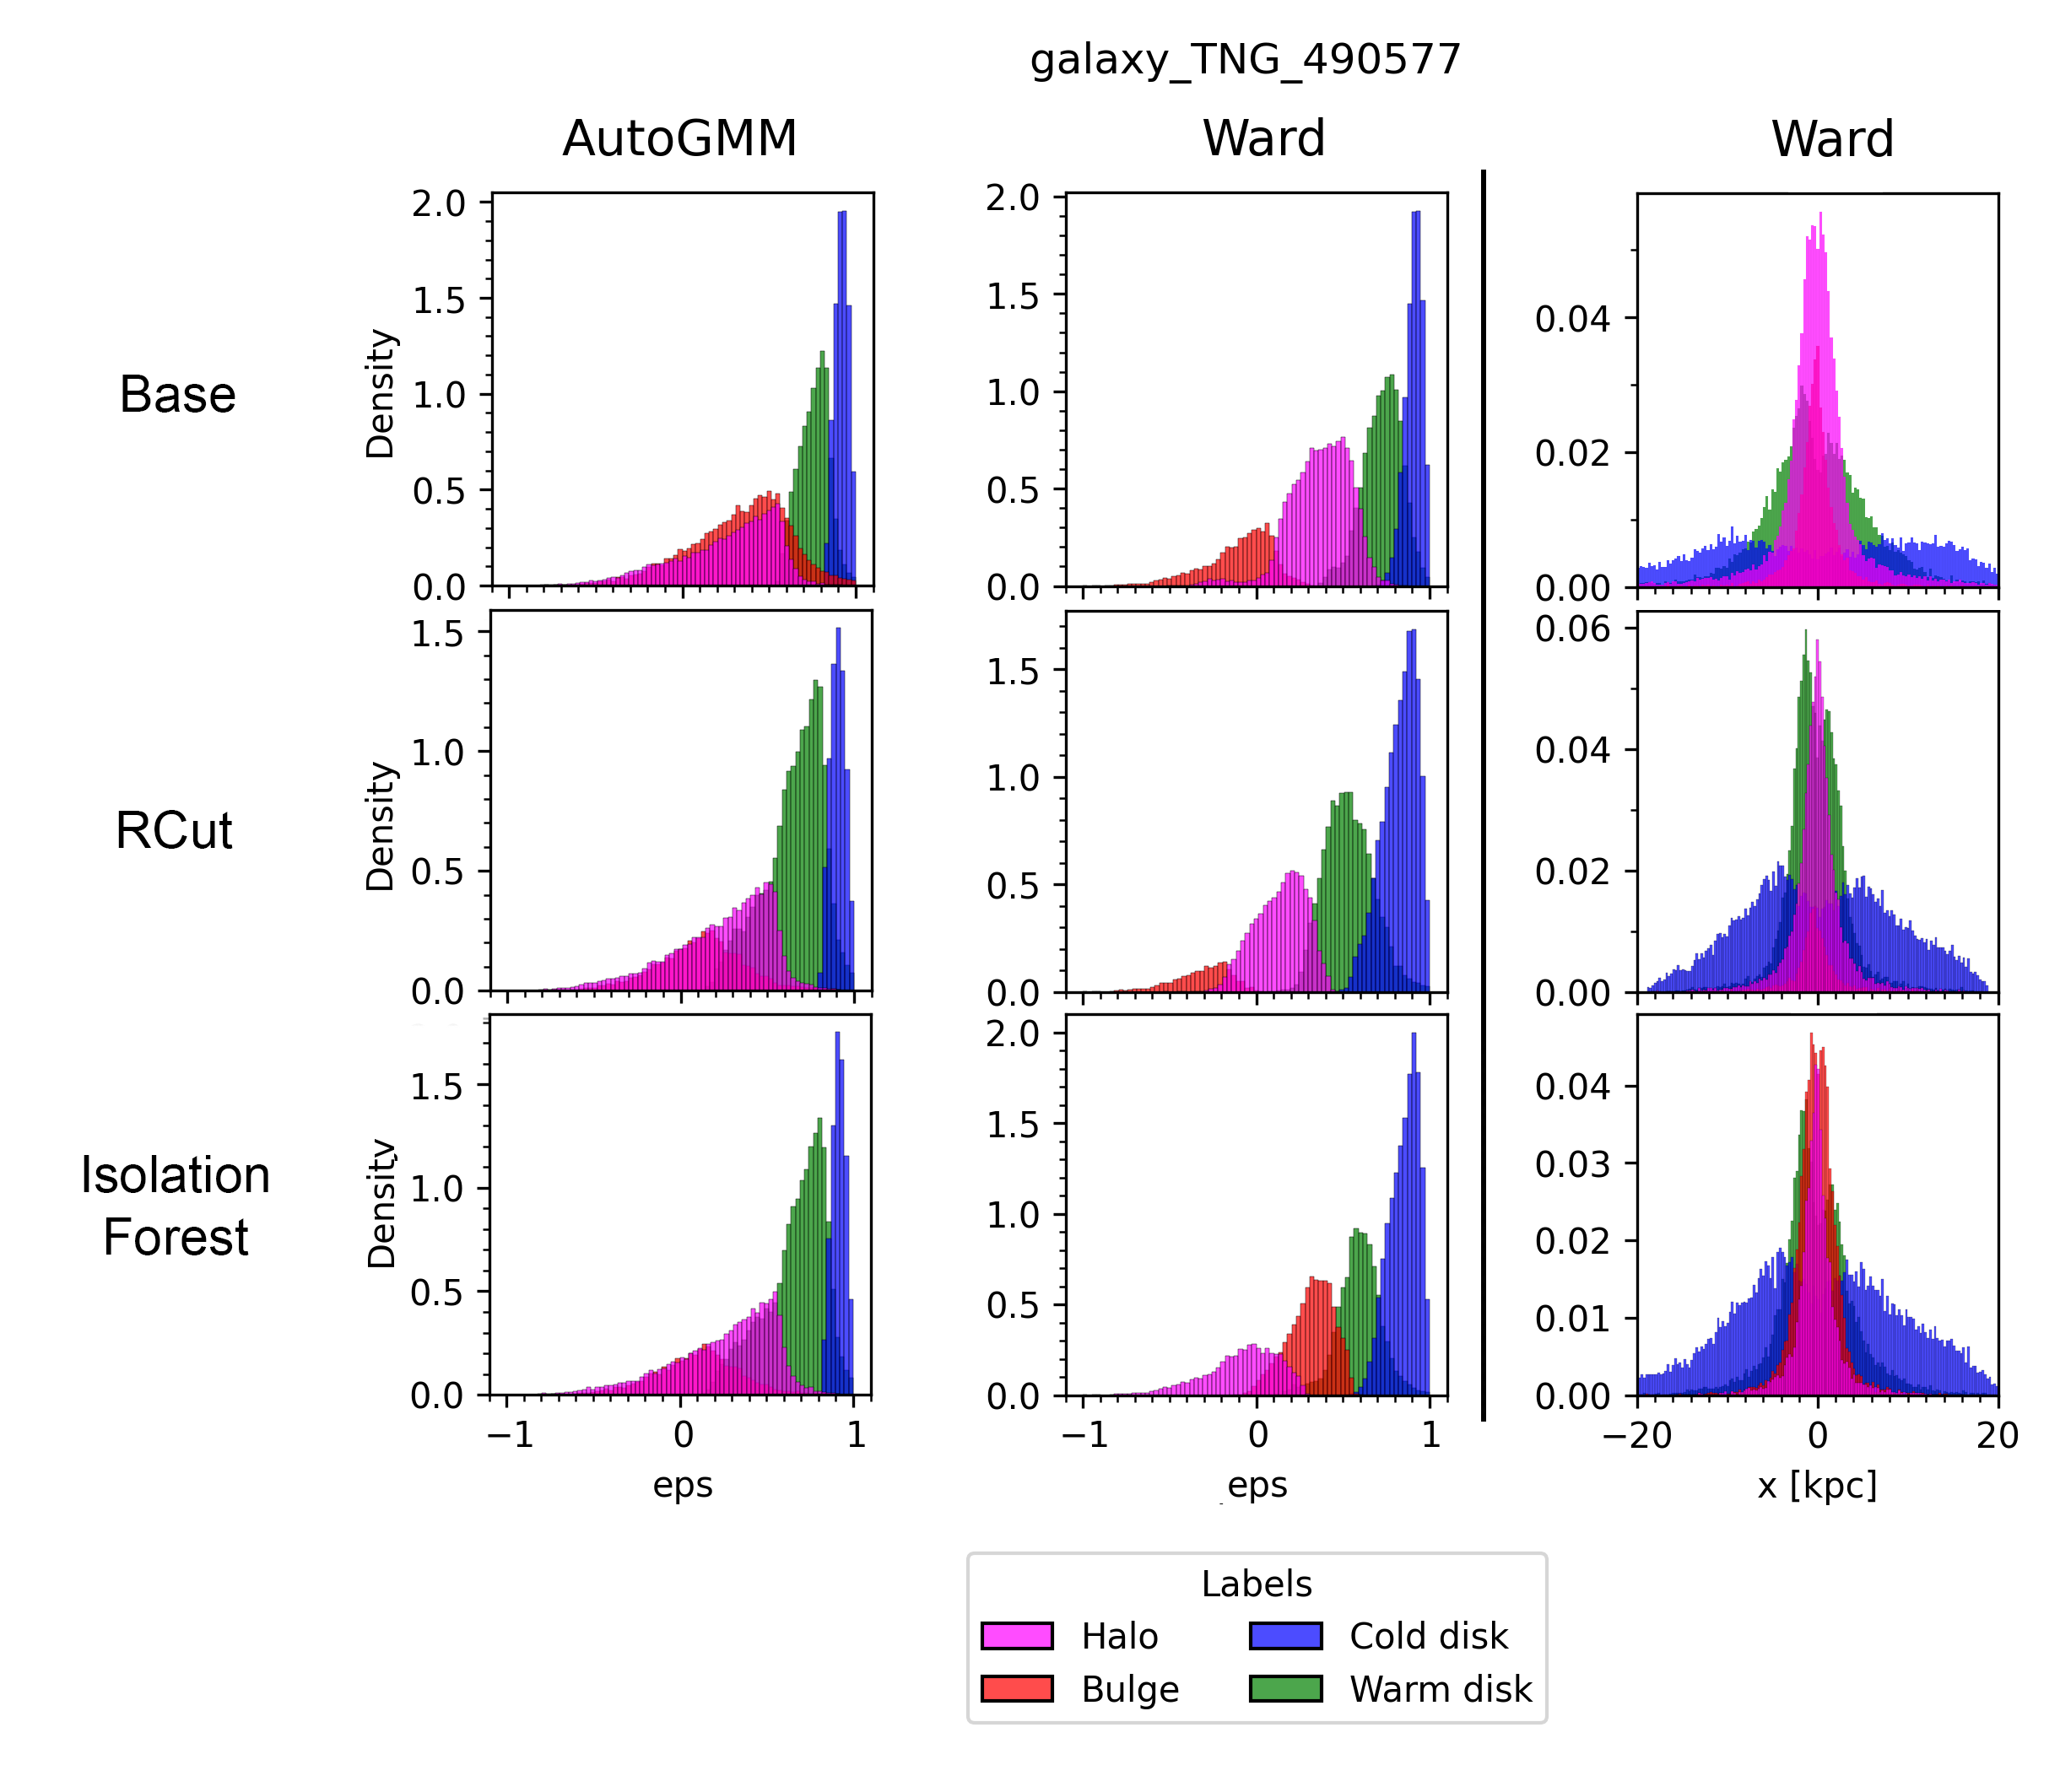
\includegraphics[width=9cm]{clustering jerarquico/figures/AGMM - galaxy_TNG_490577 - complete.png}
\end{center}

\note{
%- heuristica para asignar labels: maximiza el promedio pesado de los valores de Recall de cada conjunto encontrado de entre todas sus posibles permutaciones\\
%- aunque pareciera que hemos etiquetado de forma errónea al Halo y el Bulge en \gls{IF}, el método detallado nos provee una base sólida para razonar sobre los resultados. \\
- en el apendice tenemos mas ejemplos, pero dadas las galaxias cuya cardinalidad de componentes no vario al remover analisis (menos de la mitad de nuestro adataset), \textbf{no podemos concluir} tampoco si hacerlo nos da mejores o peores resultados.
}

\end{frame}

\iflong
\begin{frame}
\frametitle{AGMM: Eliminación de outliers}
\begin{center}
    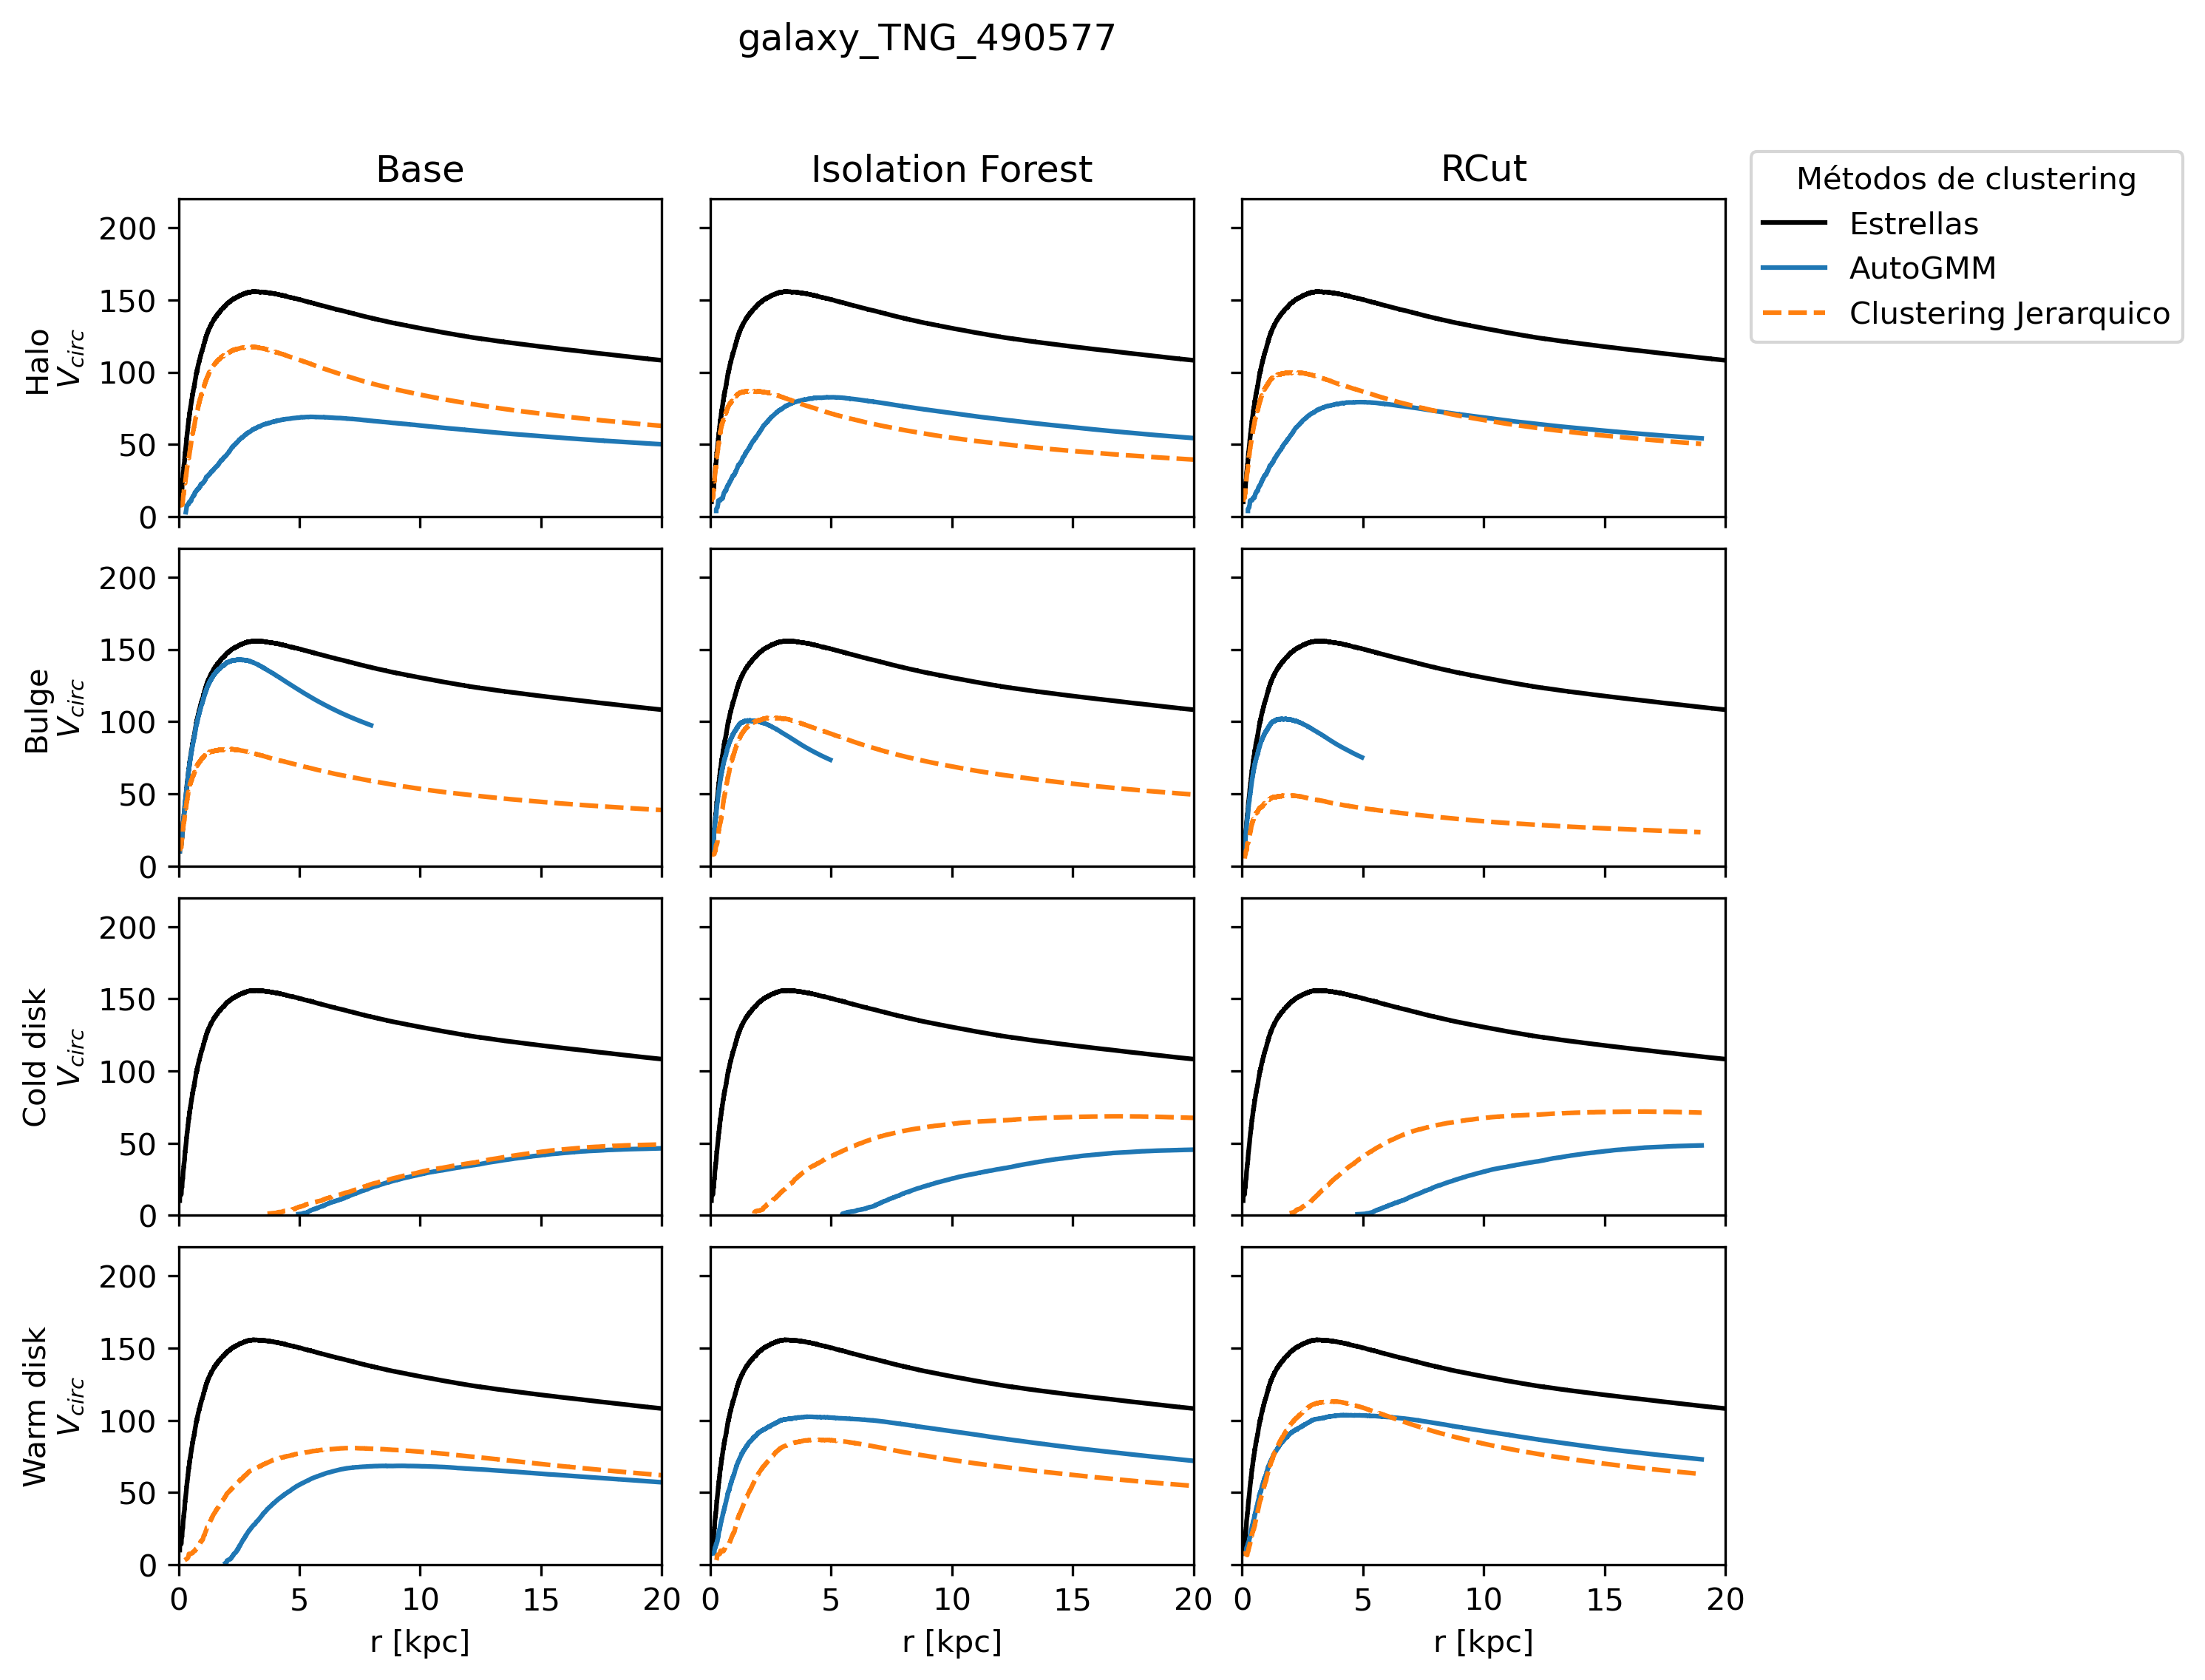
\includegraphics[width=10cm]{clustering jerarquico/figures/galaxy_TNG_490577 - AutoGMM - circ_velocity.png}
\end{center}

\note{
otro ejemplo
}

\end{frame}
\endif




\section{Fuzzy Clustering}

\begin{frame}
\frametitle{Fuzzy Clustering}

\pause

Dado $X = (x_1, x_2,..., x_k)$, con $k$ puntos de datos y $c$ clusters. \\

\pause
Definimos la función de pertenencia como:

\begin{equation}
    \begin{aligned}
        \mu_{ij} = \mu_i(x_j) \in [0, 1] \ \ \forall i = 1,...,c \land \forall j = 1,...,k
    \end{aligned}
\end{equation} 

\pause

De forma tal que:
%
\begin{equation}
    \begin{aligned}
        \sum_{i=1}^{c} \mu_i(x_j) = 1 \ \ \forall j = 1,...,k
    \end{aligned}
\end{equation} 

\note{
Es un método de clustering en el cual cada punto de los datos puede \textbf{pertenecer a más de un cluster}, mediante la asignación de valores de pertenencia a cada punto de nuestros datos por cada cluster que estemos buscando. Así, puntos cerca del borde de un cluster obtienen un bajo valor de pertenencia.
}

\end{frame}

\begin{frame}
\frametitle{Fuzzy Clustering}

Luego, definimos el conjunto de particiones difusas de la siguiente manera:

\begin{equation}
    \begin{aligned}
        M_{fc} = \{U \in \Re^{cxk} | U = [u_{ij}];u_{ij} \in [0, 1] \forall i, j; \sum_{i=1}^{c} u_{ij} = 1  \forall j; \sum_{j=1}^{k} u_{ij} > 0  \forall i \}
    \end{aligned}
\end{equation}

\pause

Función de error mínimo cuadrático:

\begin{equation}
    \begin{aligned}
        J_m(U, v) = \sum_{j=1}^{k} \sum_{i=1}^{c} (u_{ij})^m d_{ij}^2
    \end{aligned}
\end{equation} 

\begin{itemize}
    \item $d_{ij}$: Distancia Euclidiana entre el elemento $x_j$ y el centro del cluster $i$
    \item $U \in M_{fc}$: Contiene todos los pesos $u_{ij}$ asociados a las distancias cuadradas
    \item $v$: El vector centro de cada cluster
    \item $m$: Valor de fuzzines
\end{itemize}

\note{
%- Partición difusa: La caracterización de la participación de cada muestra en todos los clusters a partir de un valor de pertenecía que va de $[0, 1]$. Estas particiones difusas se representan con una matriz, asociando cada fila a uno de los $c$ clusters y cada columna a uno de los elementos de $X$, de forma tal que el valor en la fila $i$ y la columna $j$ indique la pertenencia del elemento $j$ al cluster $i$ \\
- Que representa una particion difusa (sus elementos)
\pause

- Podemos \textbf{traducir el problema} de FCM a buscar una particion difusa (es decir, una matriz perteneciente al conjunto descrito arriba) \textbf{"optima"}
}
\end{frame}


\begin{frame}
\frametitle{Fuzzy Clustering}

Algoritmo:

\begin{enumerate}
  \item <1-> Fijar $c$, $k$ y $m$. Elegir una matriz inicial $U^{(0)}\in M_{fc}$
  \item <2-> Calcular los centros de los clusters como $v_{i}={\frac {\sum \limits _{j=1}^{k}(u_{ij})^{m}x_{j}}{\sum \limits _{j=1}^{k}(u_{ij})^{m}}};1\leq i\leq c$
  \item <3-> Actualizar la matriz de partición difusa $U = [uij]$ con $u_{ij}=(\sum \limits _{n=1}^{c}({\frac {d_{ij}}{d_{nj}}})^{\frac {2}{m-1}})^{-1};1\leq j\leq k;1\leq i\leq c$
  \item <4-> Si se alcanzo la máxima cantidad de iteraciones, o la diferencia de la matriz U con respecto a la iteración anterior es menor al error mínimo dado, el algoritmo termina. Caso contrario, vuelve al paso 2.
\end{enumerate}

\note{
- $m \rightarrow 1 = kmeans$, $m \rightarrow \infty =$ el mismo valor de pertenencia para todos los clusters \\
- Una vez terminado de correr el algoritmo, \textbf{etiquetamos} cada dato de nuestro conjunto con el cluster cuyo valor en la \textbf{partición difusa sea mayor}. \\
}

\end{frame}



\begin{frame}
\frametitle{Librería utilizada}

\begin{center}
    
\includegraphics[width=7cm]{fuzzy clustering/figures/scikit-fuzzy.png}
    \href{https://pythonhosted.org/scikit-fuzzy/}{https://pythonhosted.org/scikit-fuzzy/}
\end{center}

\end{frame}


\begin{frame}
\frametitle{Abadi: Búsqueda de $m$}


\begin{columns}
\column{0.4\textwidth}

\begin{center}
    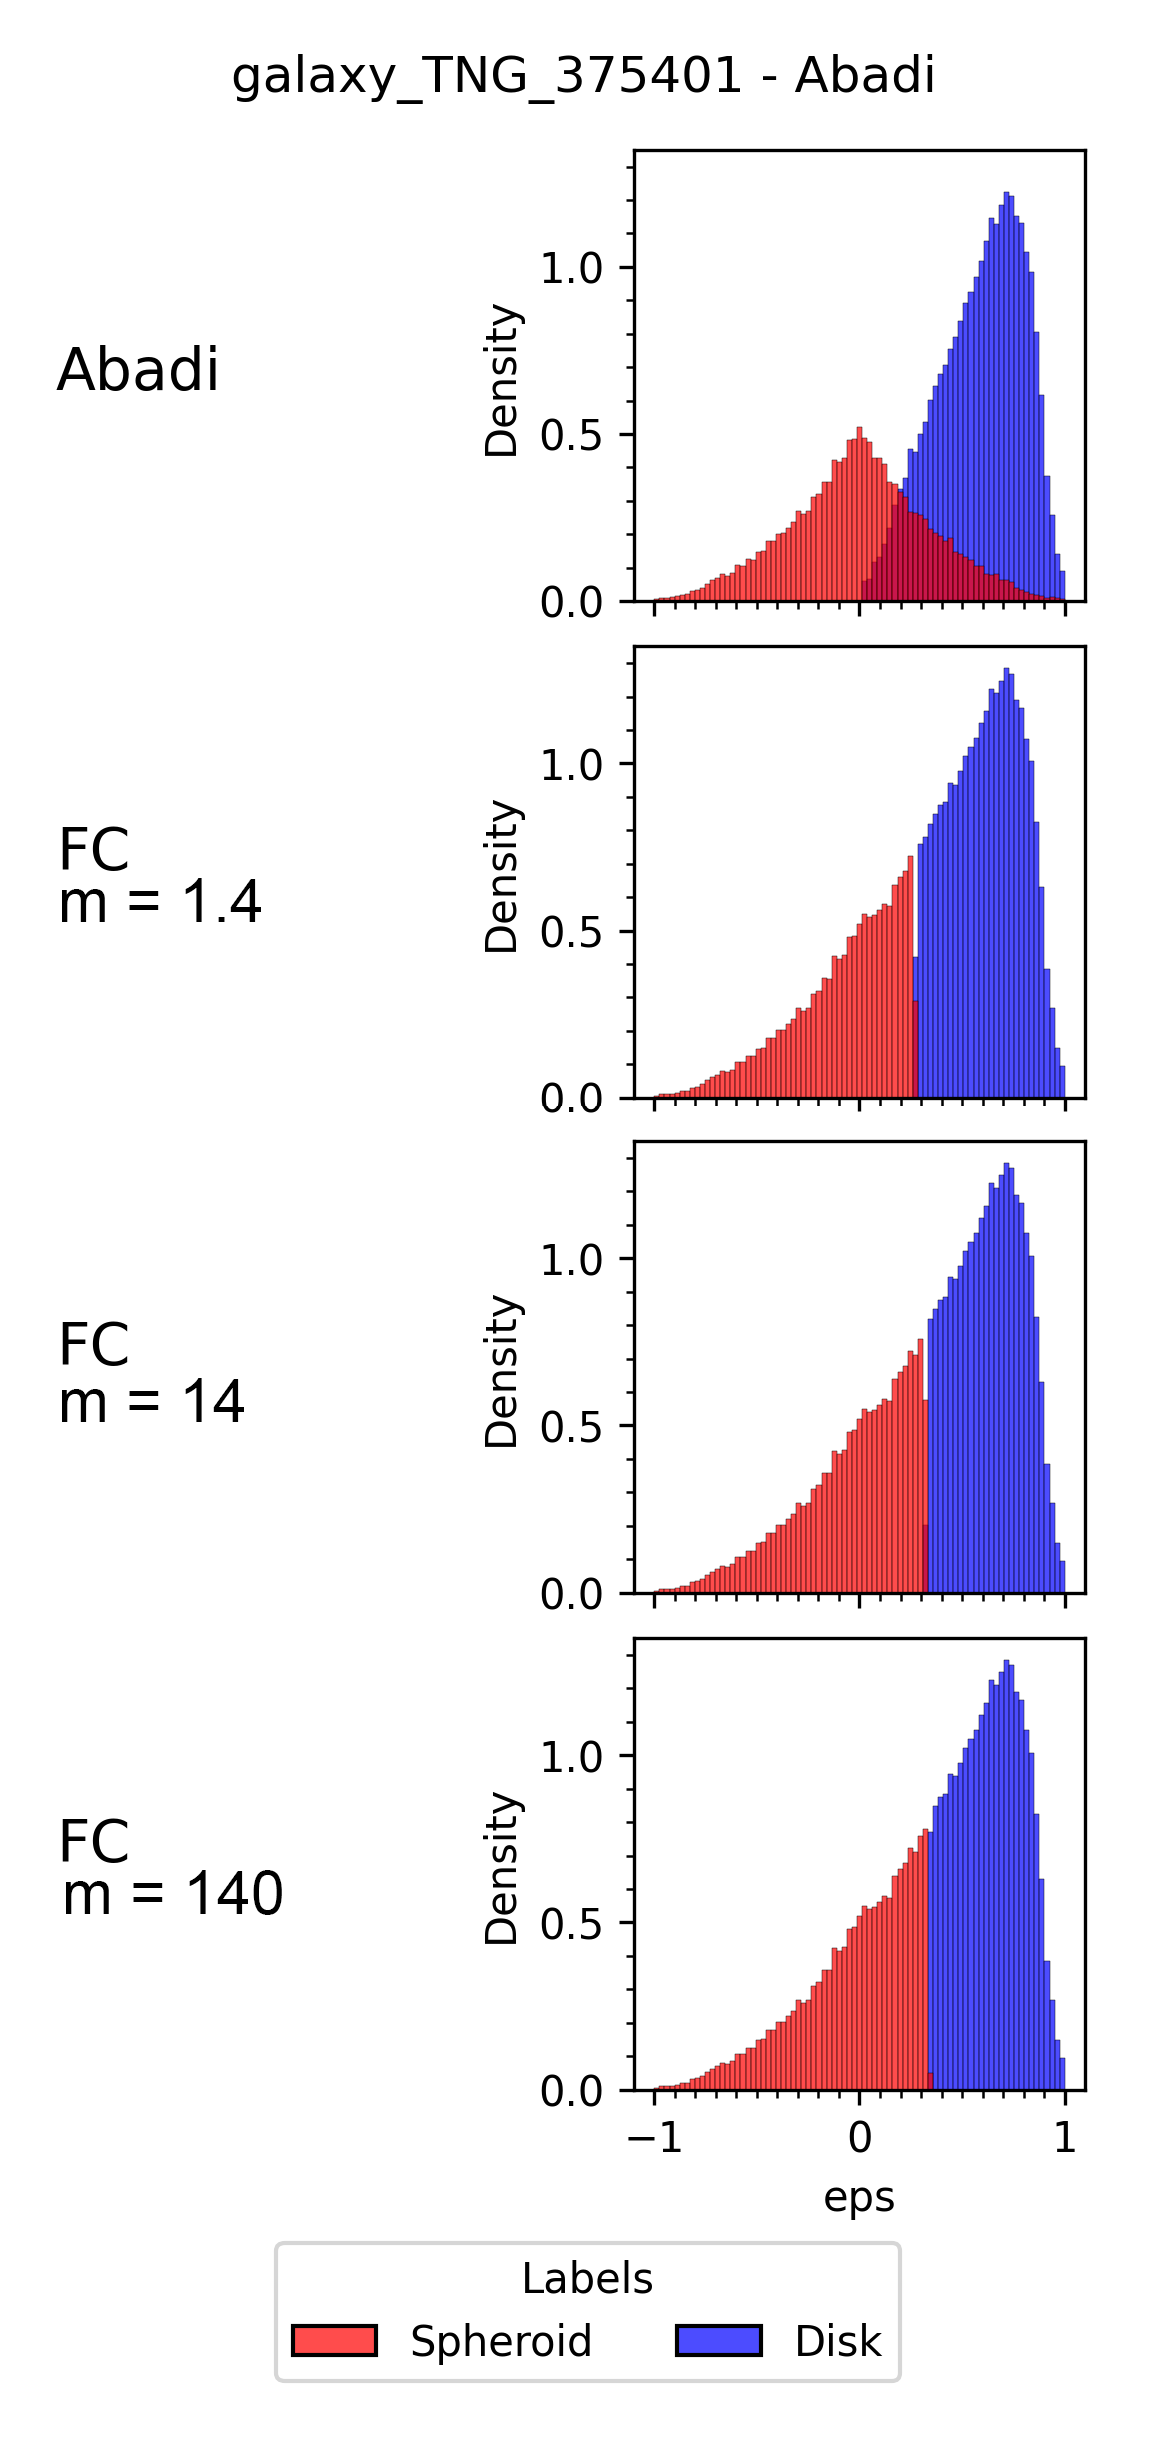
\includegraphics[width=3.8cm]{fuzzy clustering/figures/galaxy_TNG_375401 - Abadi - circ histogram fuzzines comparison.png}
\end{center}

\column{0.6\textwidth}

\begin{table}
\centering
\begin{tabular}{|c|c|}
\hline
Fuzziness&Centro de Esferoide\\
\hline
$1.4$ & $-0.078$\\
\hline
$14$ & $0.008$\\
\hline
$140$ & $0.027$\\
\hline
\end{tabular}

\end{table}

%\pause

%MAX VALUE \texttt{float64} = $2.225 \times 10^{-308}$ \\
%Q1 $u_{ij}$ (con $i$ = Disk) = $7.56 \times 10^{-5}$ \\
%m = $75$

\end{columns}

\note{
%- recordamos que como usamos una sola feature no vamos a tener mas informacion para mezclar los resultados con fuzzines\\
%- porque se \textbf{mueve la recta hacia la derecha} al aumentar m? Mirar la segunda ecuacion, aumentar m decrementa el peso que tiene xj para calcular el centro del cluster. \\
%- En la libreria los valores de pertenencia estan guardados en float64. Si separamos en quartiles ordenando por el valor de pertenencia de cada componente nos encontramos con que Q1 del disco tiene ese valor, que no es lo suficientemente chico, pero un m de 75 basta con hacer que sea menor al valor de arriba. \\
%- Aporte los \textbf{puntos más alejados de cada cluster} será nulos para el \textbf{segundo paso del algoritmo}, entonces las partículas que se encuentran más cercanas al extremo izquierdo de la recta no afectarán al cálculo del centro del cluster del Esferoide. Mayoria de estas particulas en el extremo izquierdo. Algo similar sucede con el Disco. \\
%- Partículas que se encuentren entre el centro del Esferoide y el Disco en la recta y las cuales antes tenían un valor de pertenencia al Disco mayor que el valor de pertenencia al Esferoide, pasen a formar parte del Esferoide, moviendo la línea de corte hacia la derecha en el proceso. \\
%- Entre más grande es el valor de fuzziness, la diferencia entre los puntos que pasaran a no formar parte del cálculo de centros de clusters entre el Esferoide y el Disco se incrementará aún más, moviendo el corte hacia la derecha en la misma medida \\
Aumentar m movia la \textbf{linea de corte} hacia la \textbf{derecha}.
}



\end{frame}





\begin{frame}
\frametitle{Abadi: Detección de 2 componentes}

Concluimos en usar:
\begin{enumerate}
    \item $m$ = 1.4
    \item Error mínimo = $0.00005$
    \item Iteraciones máximas =  $1000$
\end{enumerate}

\begin{center}
    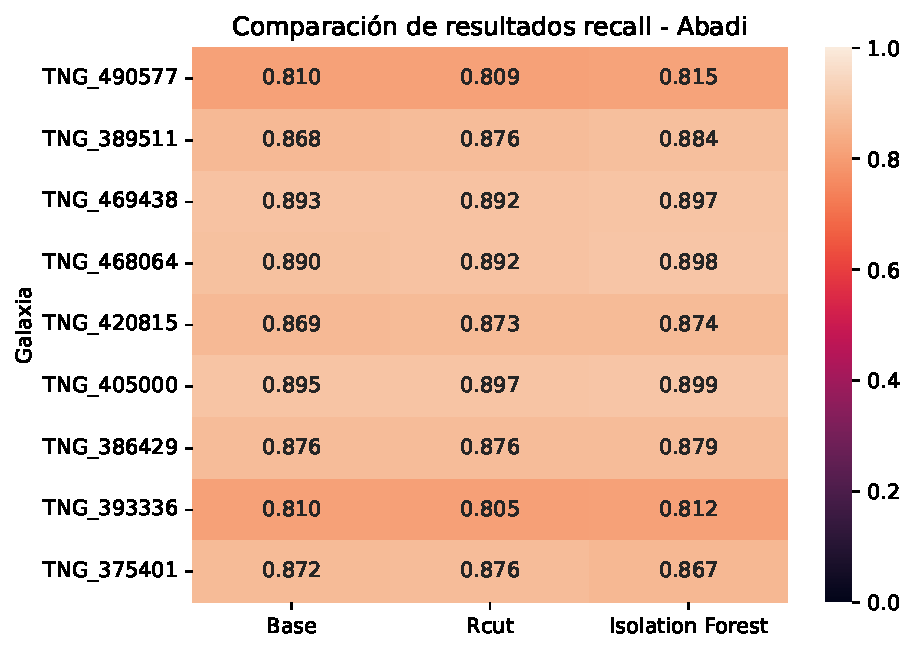
\includegraphics[width=8cm]{fuzzy clustering/figures/abadi - recall.pdf}
\end{center}

%ver mejor?
\note{
- Dado el dominio de resultados posibles, pasamos a elegir un \textbf{valor de fuzziness que acerque la linea de corte} al punto promedio en donde la densidad del Disco supera a la del Esferoide en todas las galaxias de nuestro dataset \\
- \textbf{Similar con CJ}, fuzzy es bueno al buscar 2 clusters entendiendo sus limitaciones?
}

\end{frame}




\begin{frame}
\frametitle{Abadi: Eliminación de outliers}

\begin{center}
    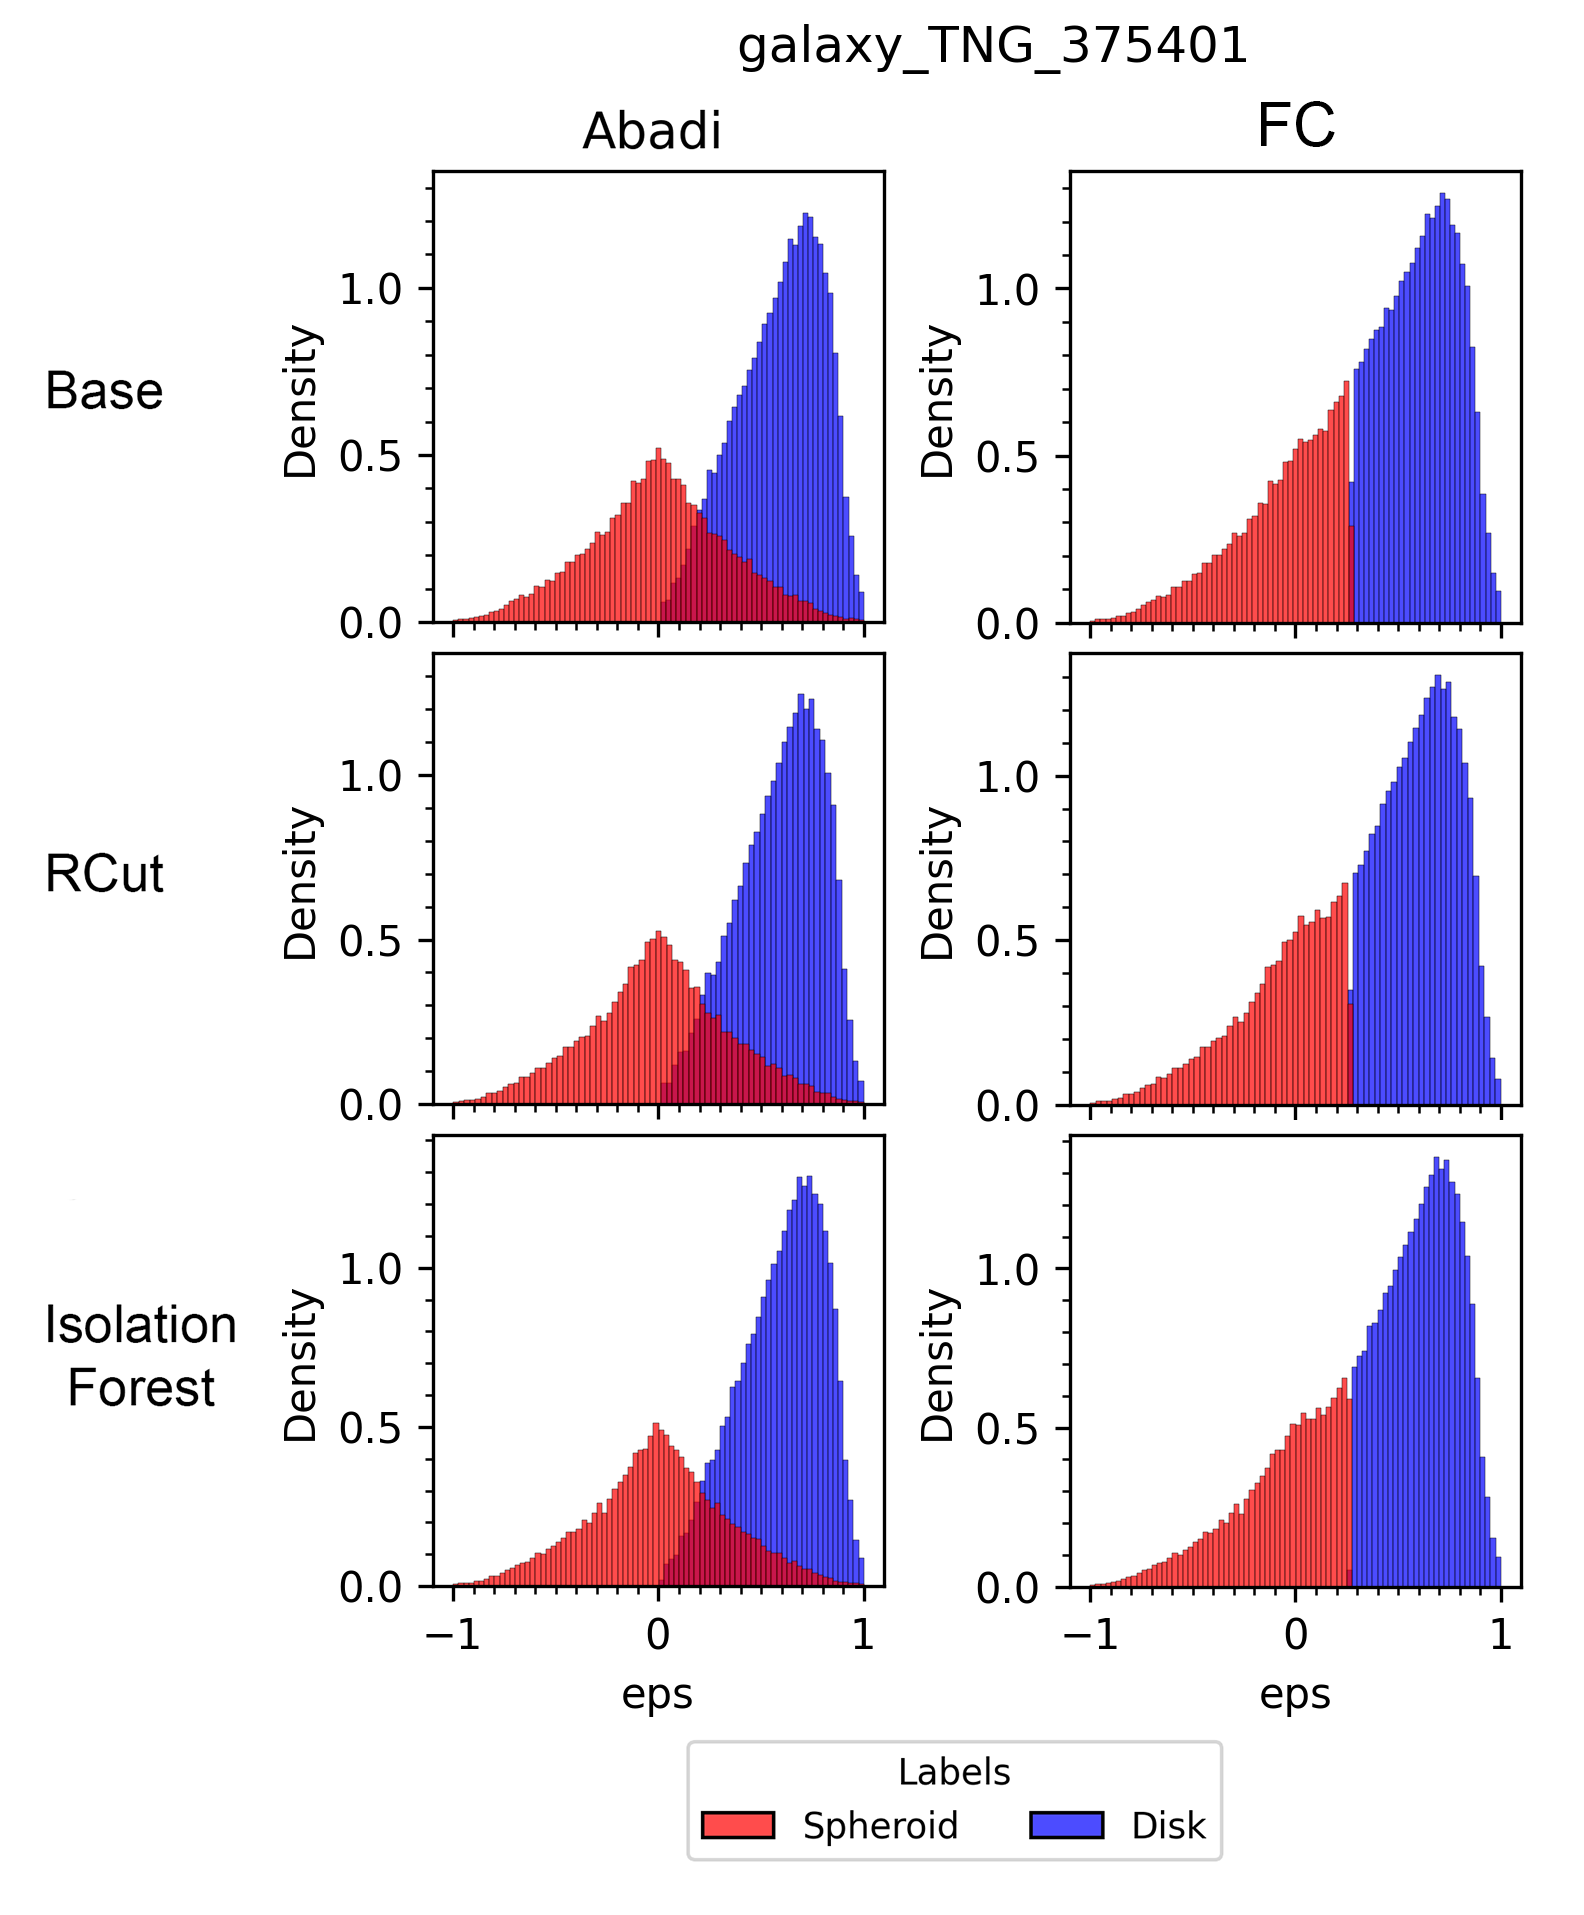
\includegraphics[width=6.5cm]{fuzzy clustering/figures/galaxy_TNG_375401 - Abadi - outlier removal comparison.png}
\end{center}

\note{
- Aplicar \gls{IF} y \gls{RCUT} \textbf{apenas si modifican} los conjuntos encontrados de forma perceptible \\
- Esto se debe a que Fuzzy clustering es un método robusto dado que \textbf{limita el impacto de los outliers} al calcular los centros de los clusters, por lo que sacarlos apenas tiene efecto
}

\end{frame}

\iflong
\begin{frame}
\frametitle{Abadi: Eliminación de outliers}

\begin{center}
    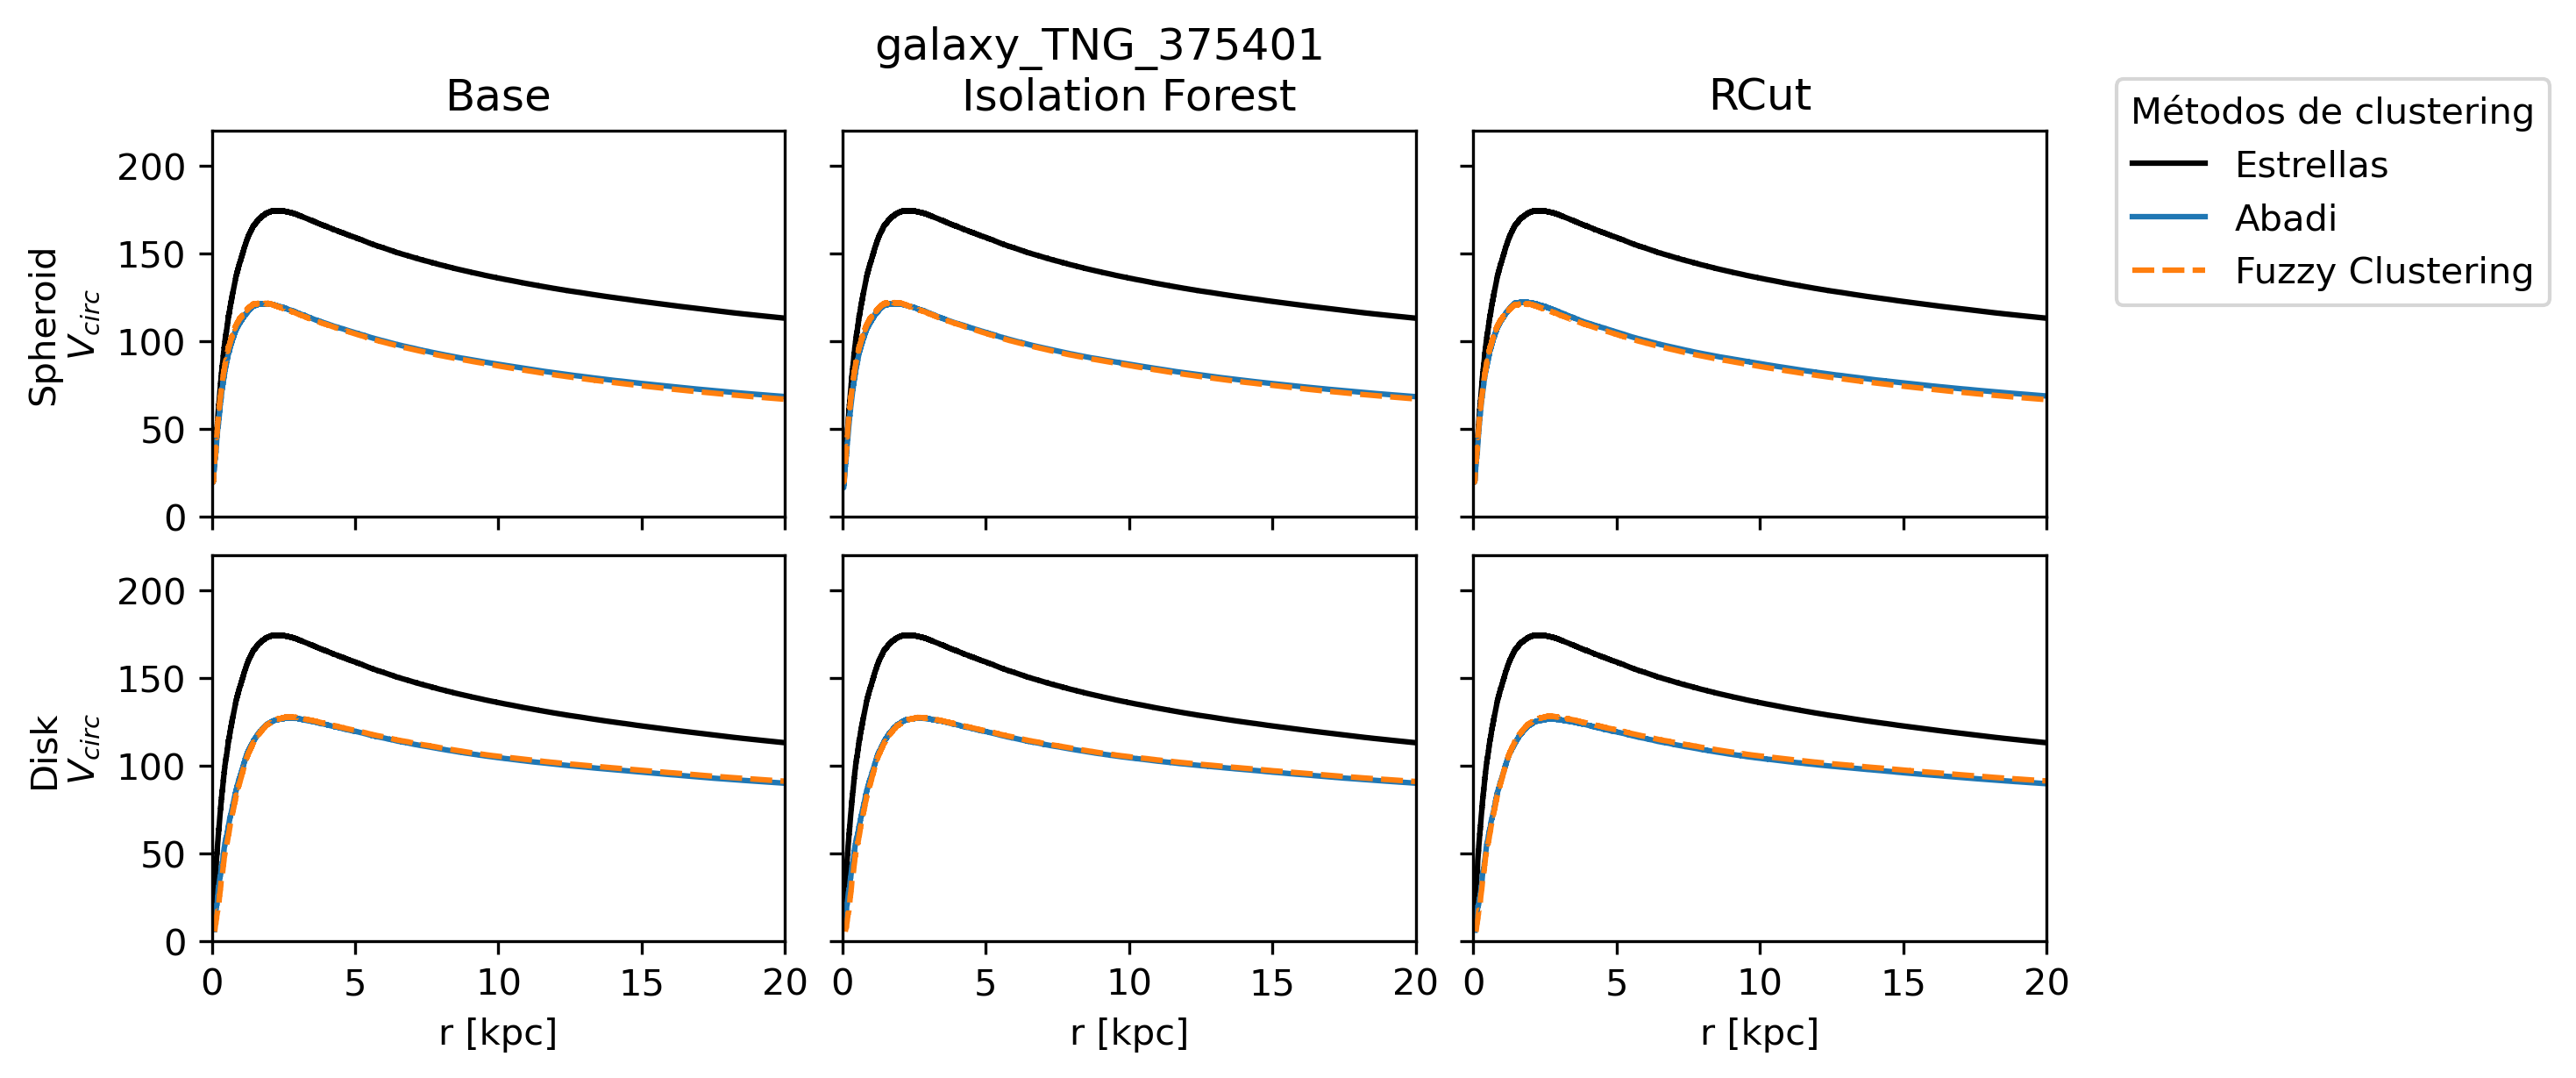
\includegraphics[width=12cm]{fuzzy clustering/figures/galaxy_TNG_375401 - Abadi - circ_velocity.png}
\end{center}

\end{frame}
\fi


\begin{frame}
\frametitle{AGMM: Detección de $>=$2 componentes}

\begin{enumerate}
    \item $m$ = 3
    \item Error mínimo = $0.00005$
    \item Iteraciones máximas =  $1000$
\end{enumerate}

\begin{center}
    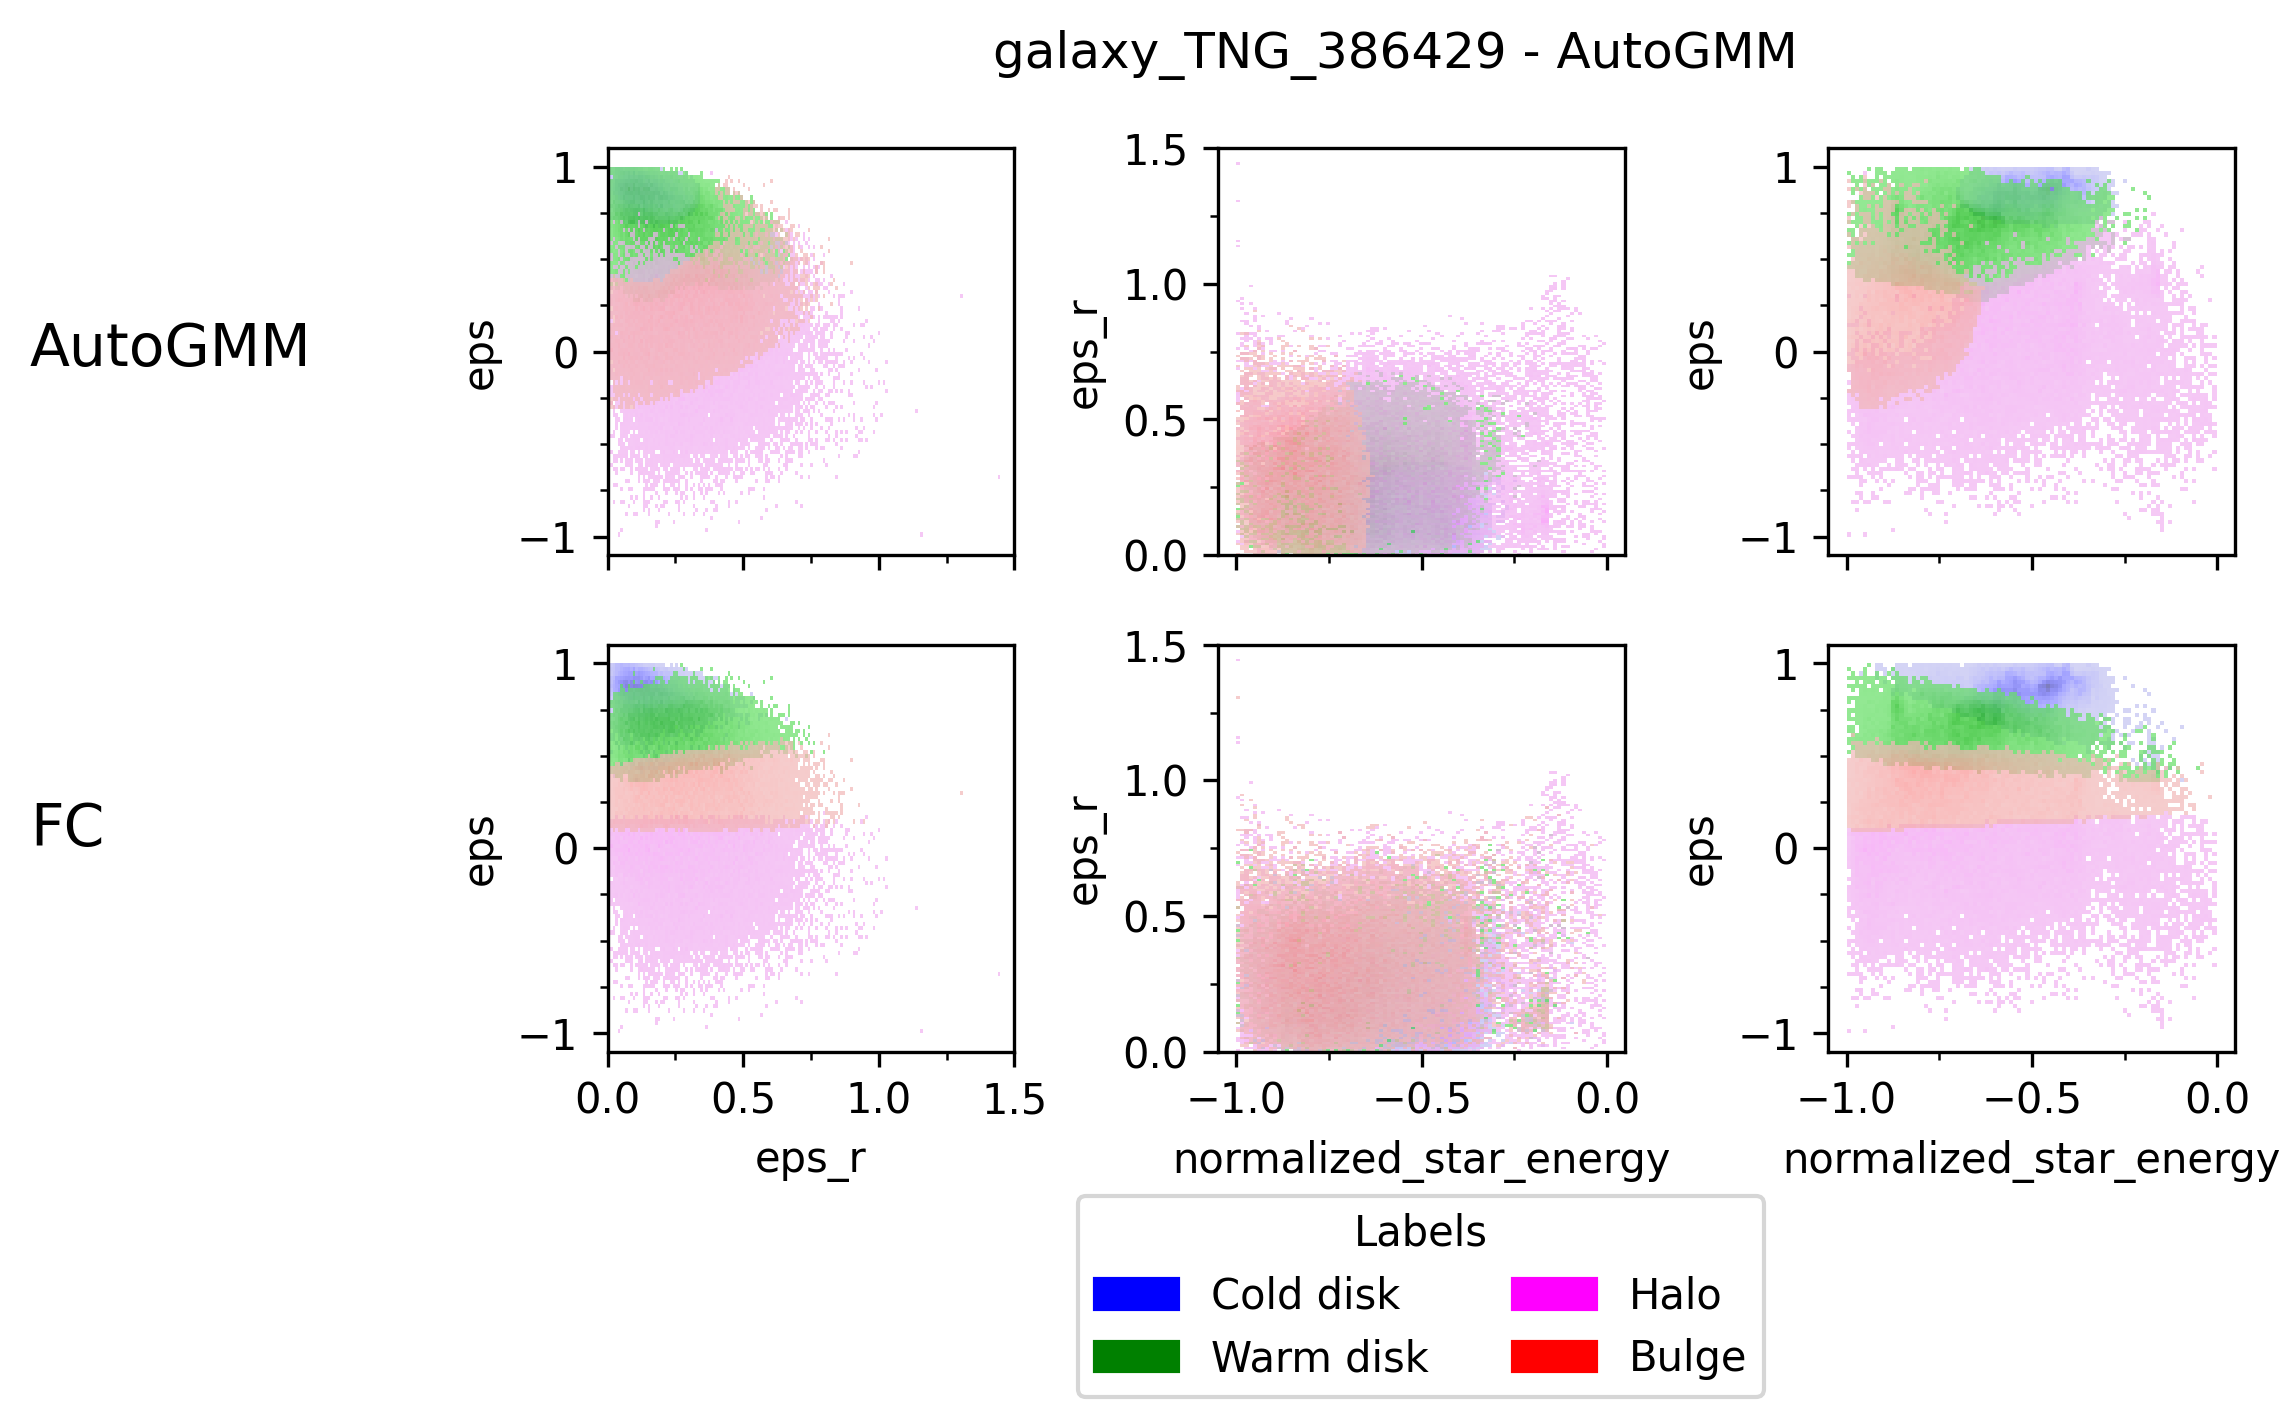
\includegraphics[width=10cm]{fuzzy clustering/figures/galaxy_TNG_386429 - circ scatterplot.png}
\end{center}
\note{
- \textbf{busqueda de m} ahora tiene el \textbf{efecto esperado} al usar mas features \\
%- lo que nos deja mas cercano a agmm, mantendremos el resto de los valores \\
- Similar a CJ, los resultados son bastante \textbf{unidimencionales} \\
- Creemos que fue por una \textbf{sobre reelevancia de features}. Aunque eps nos sirva para identificar ambos discos, necesitamos utilizar mejor \textbf{normalized\_star\_energy} para identificar el \textbf{bulge} y el \textbf{halo}, como se puede ver en el siguiente histograma (otra diapo) \\
}

\end{frame}


\begin{frame}
\frametitle{AGMM: Detección de $>=$2 componentes}

\begin{center}
    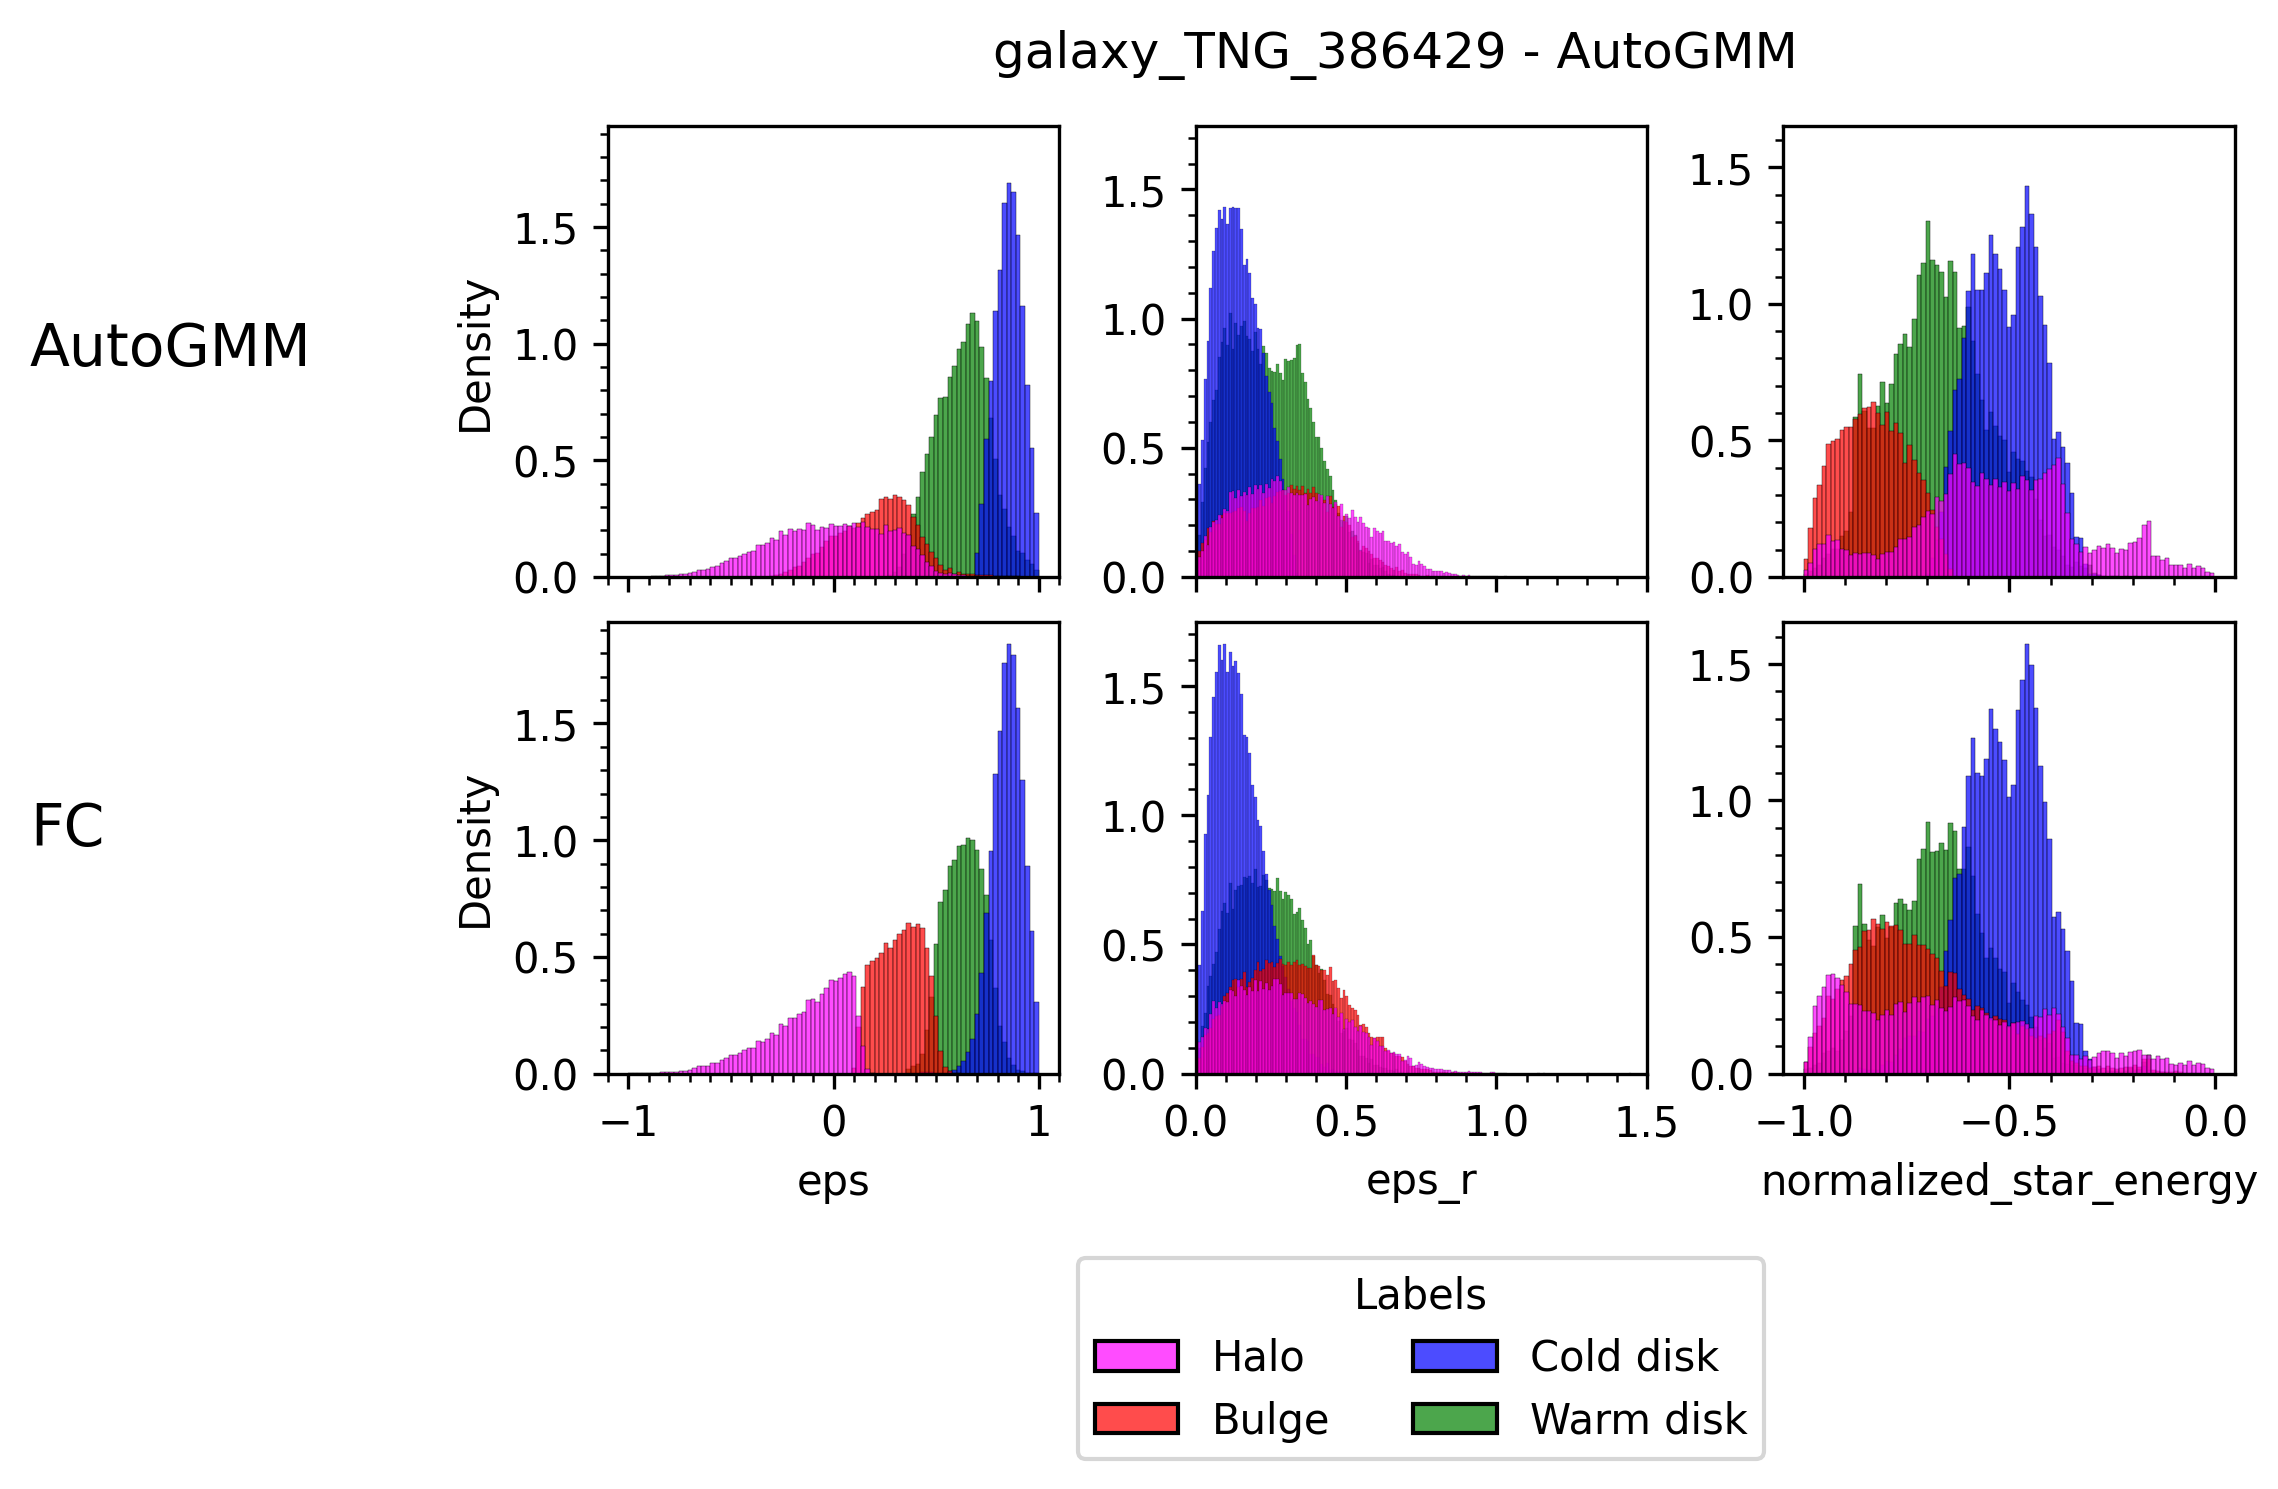
\includegraphics[width=12cm]{fuzzy clustering/figures/galaxy_TNG_386429 - circ histogram.png}
\end{center}

\note{
- Volvemos al \textbf{tercer paso del algo}, deriva el \textbf{valor de pertenencia} de cada partícula con cada cluster a partir de la \textbf{distancia} de ésta hacia el \textbf{centro de cada cluster}. \\
%- Sin embargo, observando las distribuciones de las partículas estelares podemos apreciar los \textbf{rangos de valores} que una partícula puede tener en \textbf{cada feature} (siguiente diapo)
%ponemos tabla?
%- Tabla: centro de los clusters encontrados por FCM estan mas o menos cerca de los encontrados por AGMM \\
}

\end{frame}




\begin{frame}
\frametitle{AGMM: Detección de $>=$2 componentes}
% explicar el tamaño cubierto por cada eje
\begin{center}
    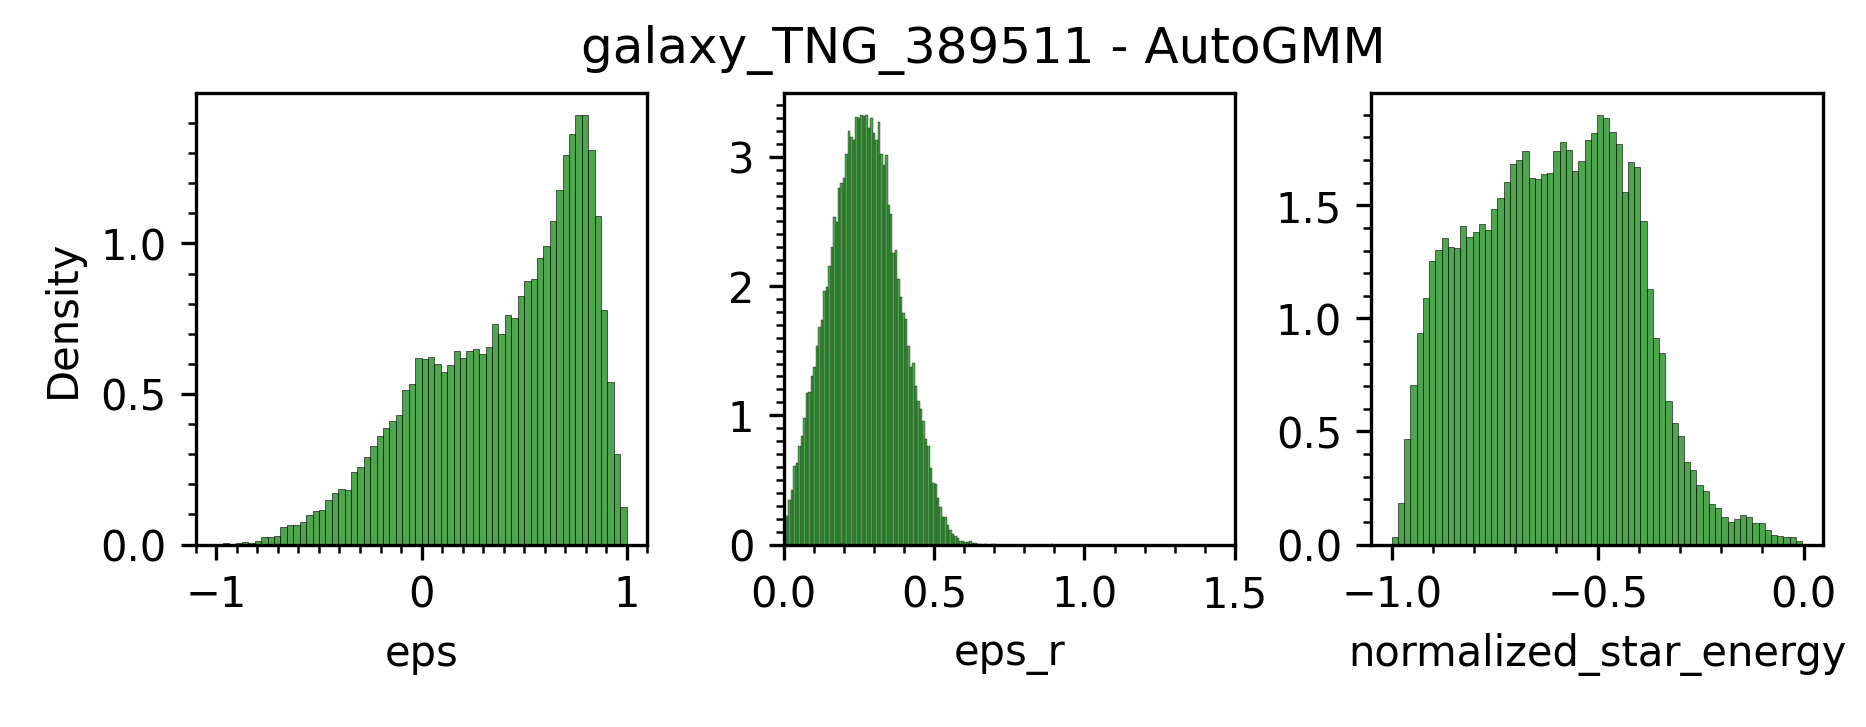
\includegraphics[width=12cm]{fuzzy clustering/figures/galaxy_TNG_389511 - circ histogram - features.png}
\end{center}

\note{
- Los valores de $eps$ tienen un rango $[-1, 1]$, mientras que el rango de los valores de $normalized\_star\_energy$ es $[-1, 0]$ y el de $eps\_r$ $[0, 1.5]$ (aunque a fines prácticos suele ser $[0, 1]$, incluso menor como se ve aca). \\
- Esto implica que haya \textbf{altas probabilidades} de que la \textbf{distancia} entre un punto a un cluster (y por consuecuente su \textbf{valor de pertenencia}) resulte fuertemente \textbf{dominado por eps}. \\
% Nuevamente, normalized star energy podria ayudar a diferenciar bulge y halo bastante \\
% eps_r no ayuda mucho \\
%- Curiosamente, podemos ver el efecto que tiene $normalized\_star\_energy$ sobre los valores de pertenencia, con las \textbf{lineas separatorias} en eps vs normalized star energy \textbf{un tanto inclinadas}. \\
%- Dicha inclinacion proviene del (leve) \textbf{aporte que hace la feature} de normalized star energy sobre el valor de pertenencia de las particulas. \\
}

\end{frame}


\iflong
\begin{frame}
\frametitle{AGMM: Detección de $>=$2 componentes}
\begin{center}
    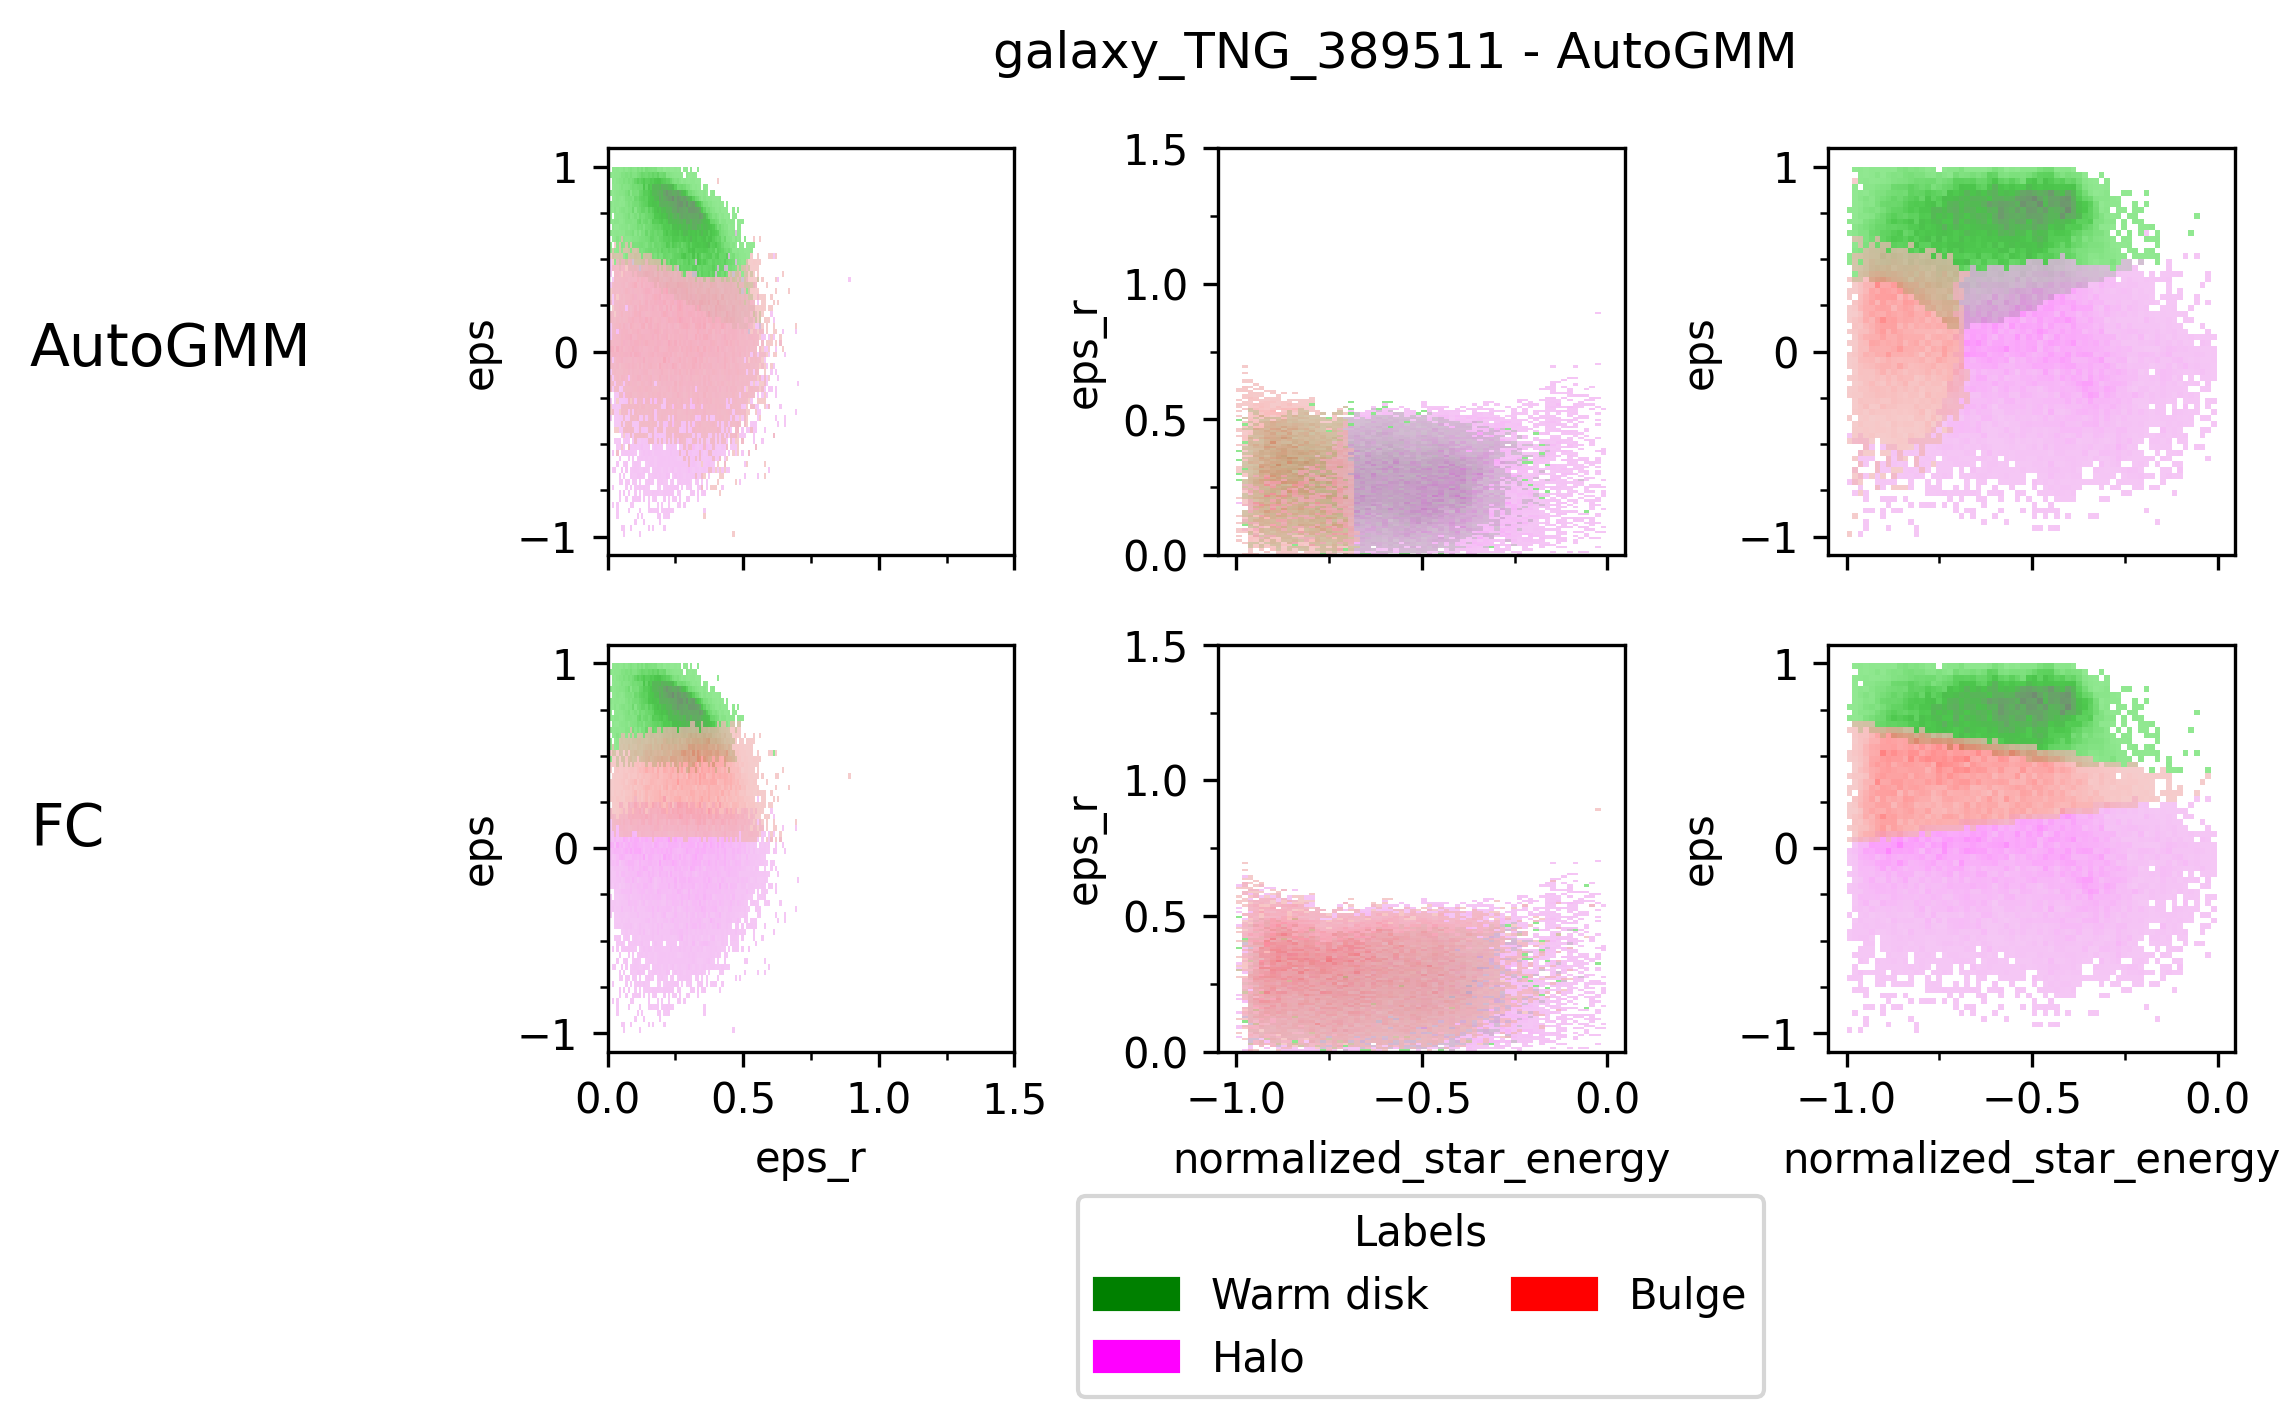
\includegraphics[width=12cm]{fuzzy clustering/figures/galaxy_TNG_389511 - circ scatterplot.png}
\end{center}

\note{
- Curiosamente, podemos ver el efecto que tiene $normalized\_star\_energy$ sobre los valores de pertenencia, con las lineas separatorias en eps vs normalized star energy un tanto inclinadas. \\
- Dicha inclinacion proviene del (leve) aporte que hace la feature de normalized star energy sobre el valor de pertenencia de las particulas. \\
- nulo aporte de eps_r en FCM, fijate lo recta que son las divisiones vs. eps \\
}

\end{frame}
\fi

\iflong
\begin{frame}
\frametitle{AGMM: Detección de $>=$2 componentes}


\begin{center}
    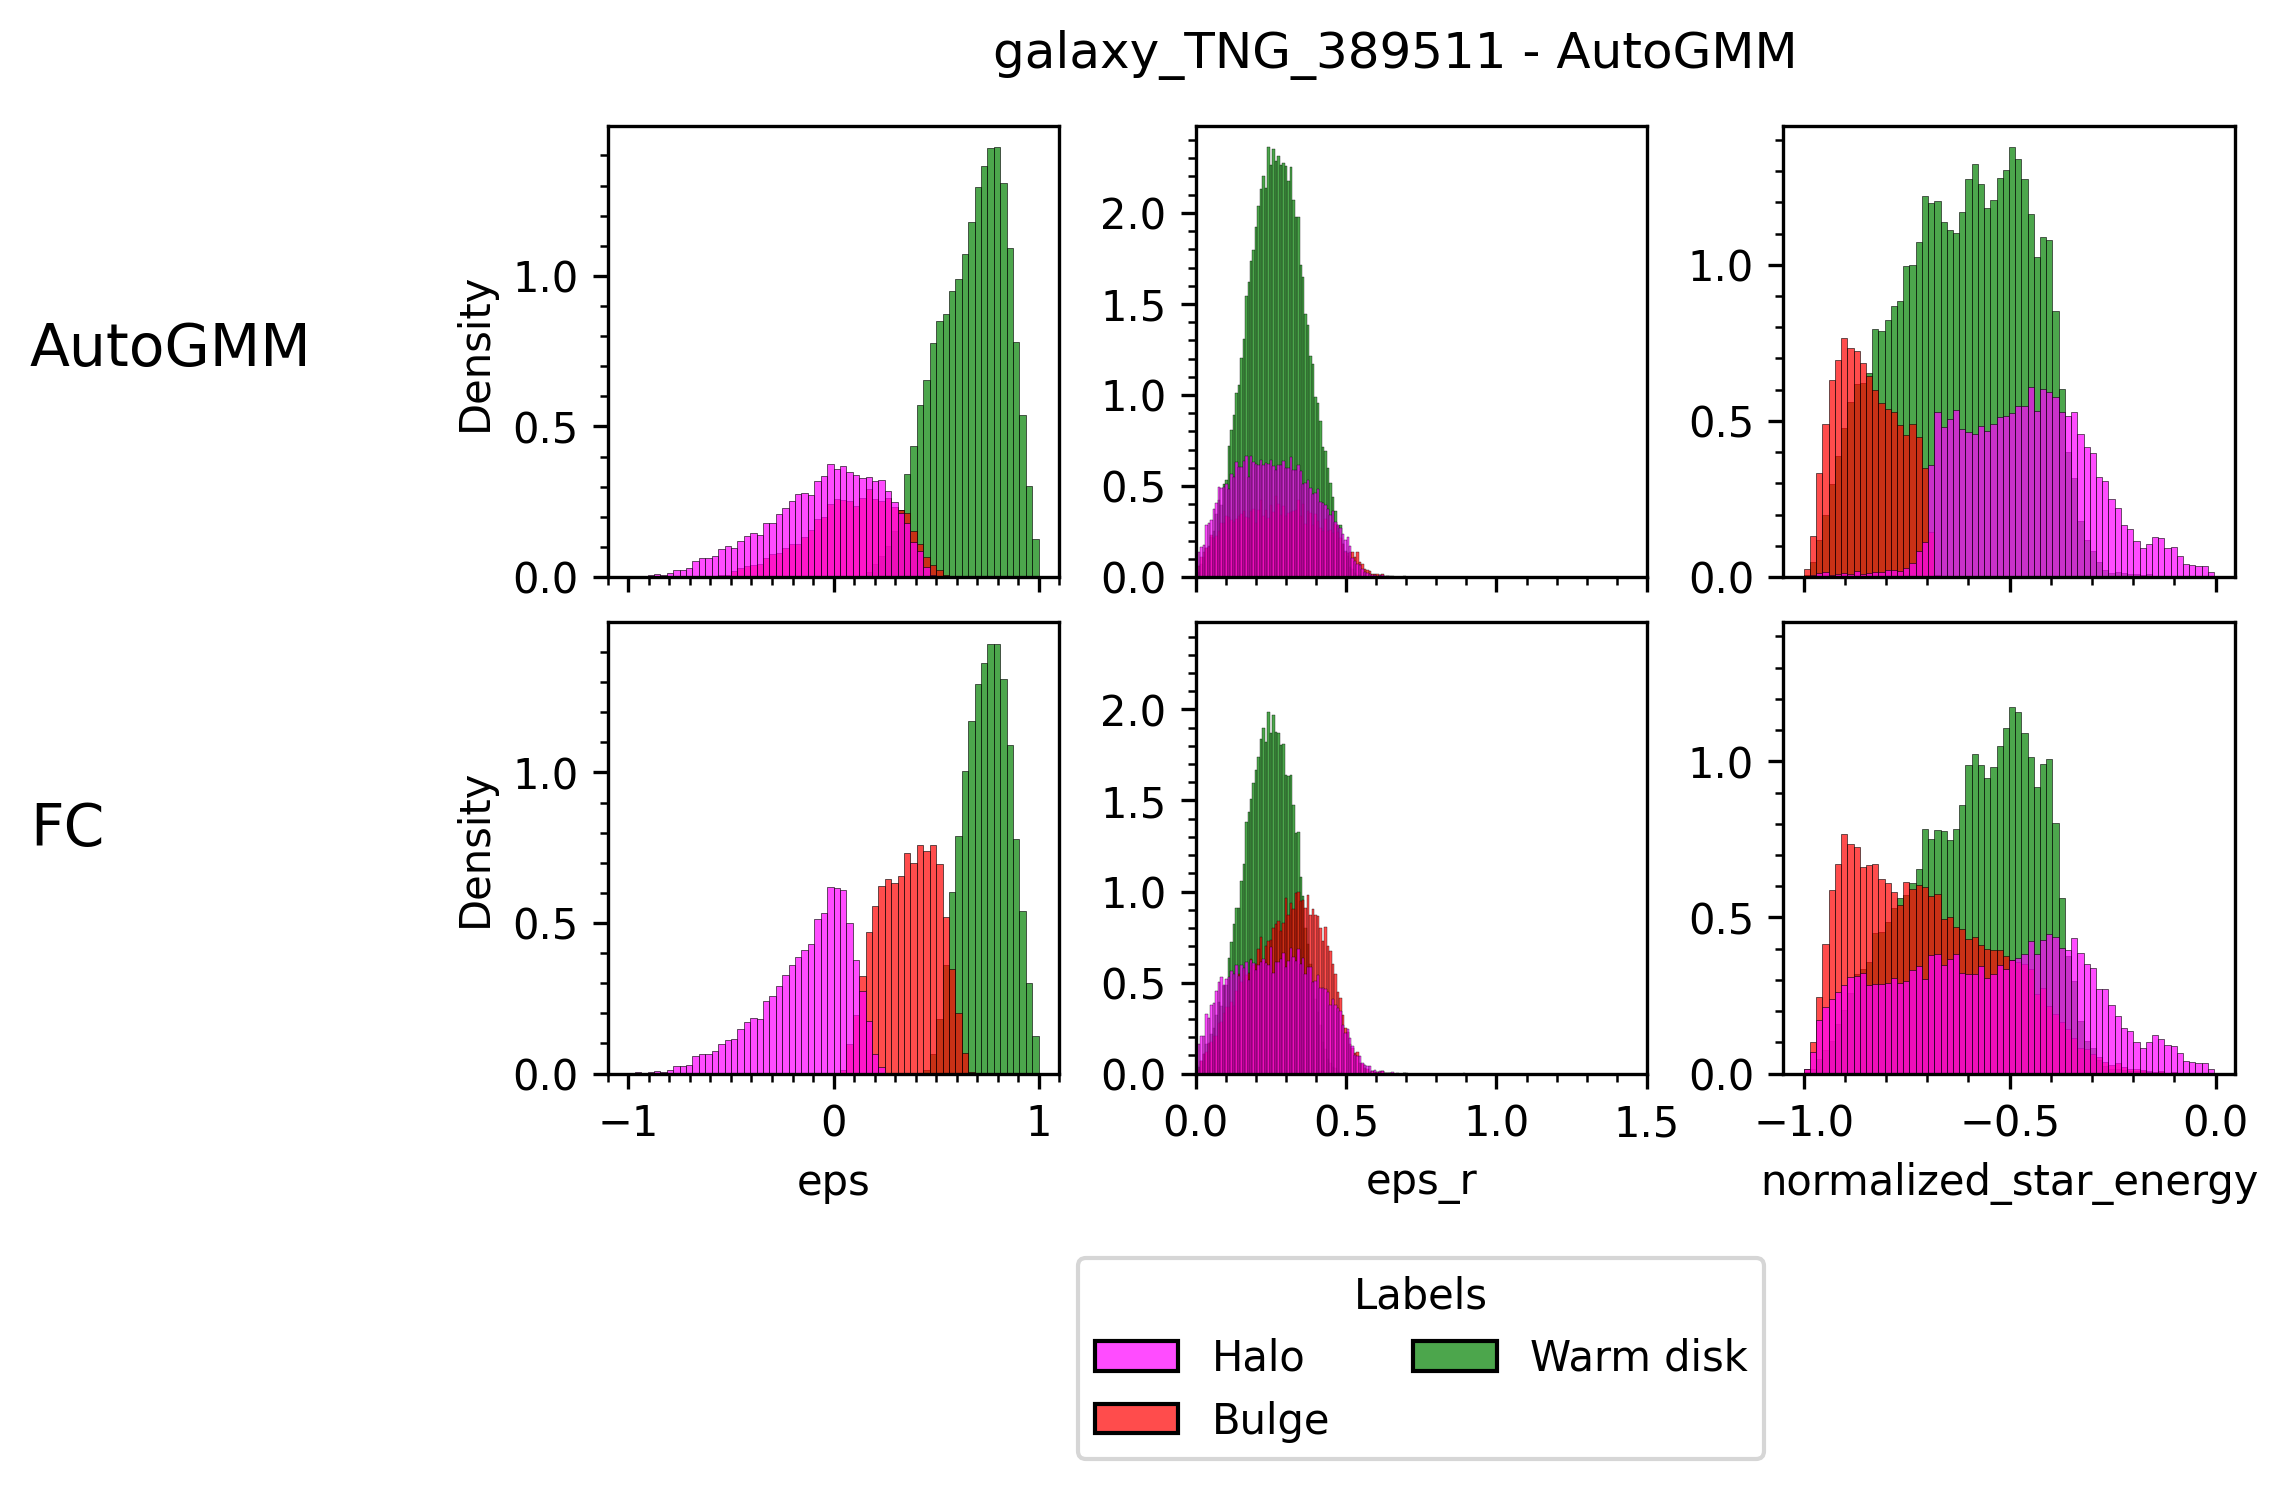
\includegraphics[width=12cm]{fuzzy clustering/figures/galaxy_TNG_389511 - circ histogram.png}
\end{center}

\note{
- Se puede ver de forma aun mas clara el poco impacto que tiene normalized star energy en la clusterizacion realizada por FCM en el histograma, y como esta es mas relevante en agmm \\
}

\end{frame}
\fi


\iflong
\begin{frame}
\frametitle{AGMM: Detección de $>=$2 componentes}

% similar a lo de la seccion anterior
% presente en graficas anteriores, pero se ve mas claro en esta

\begin{center}
    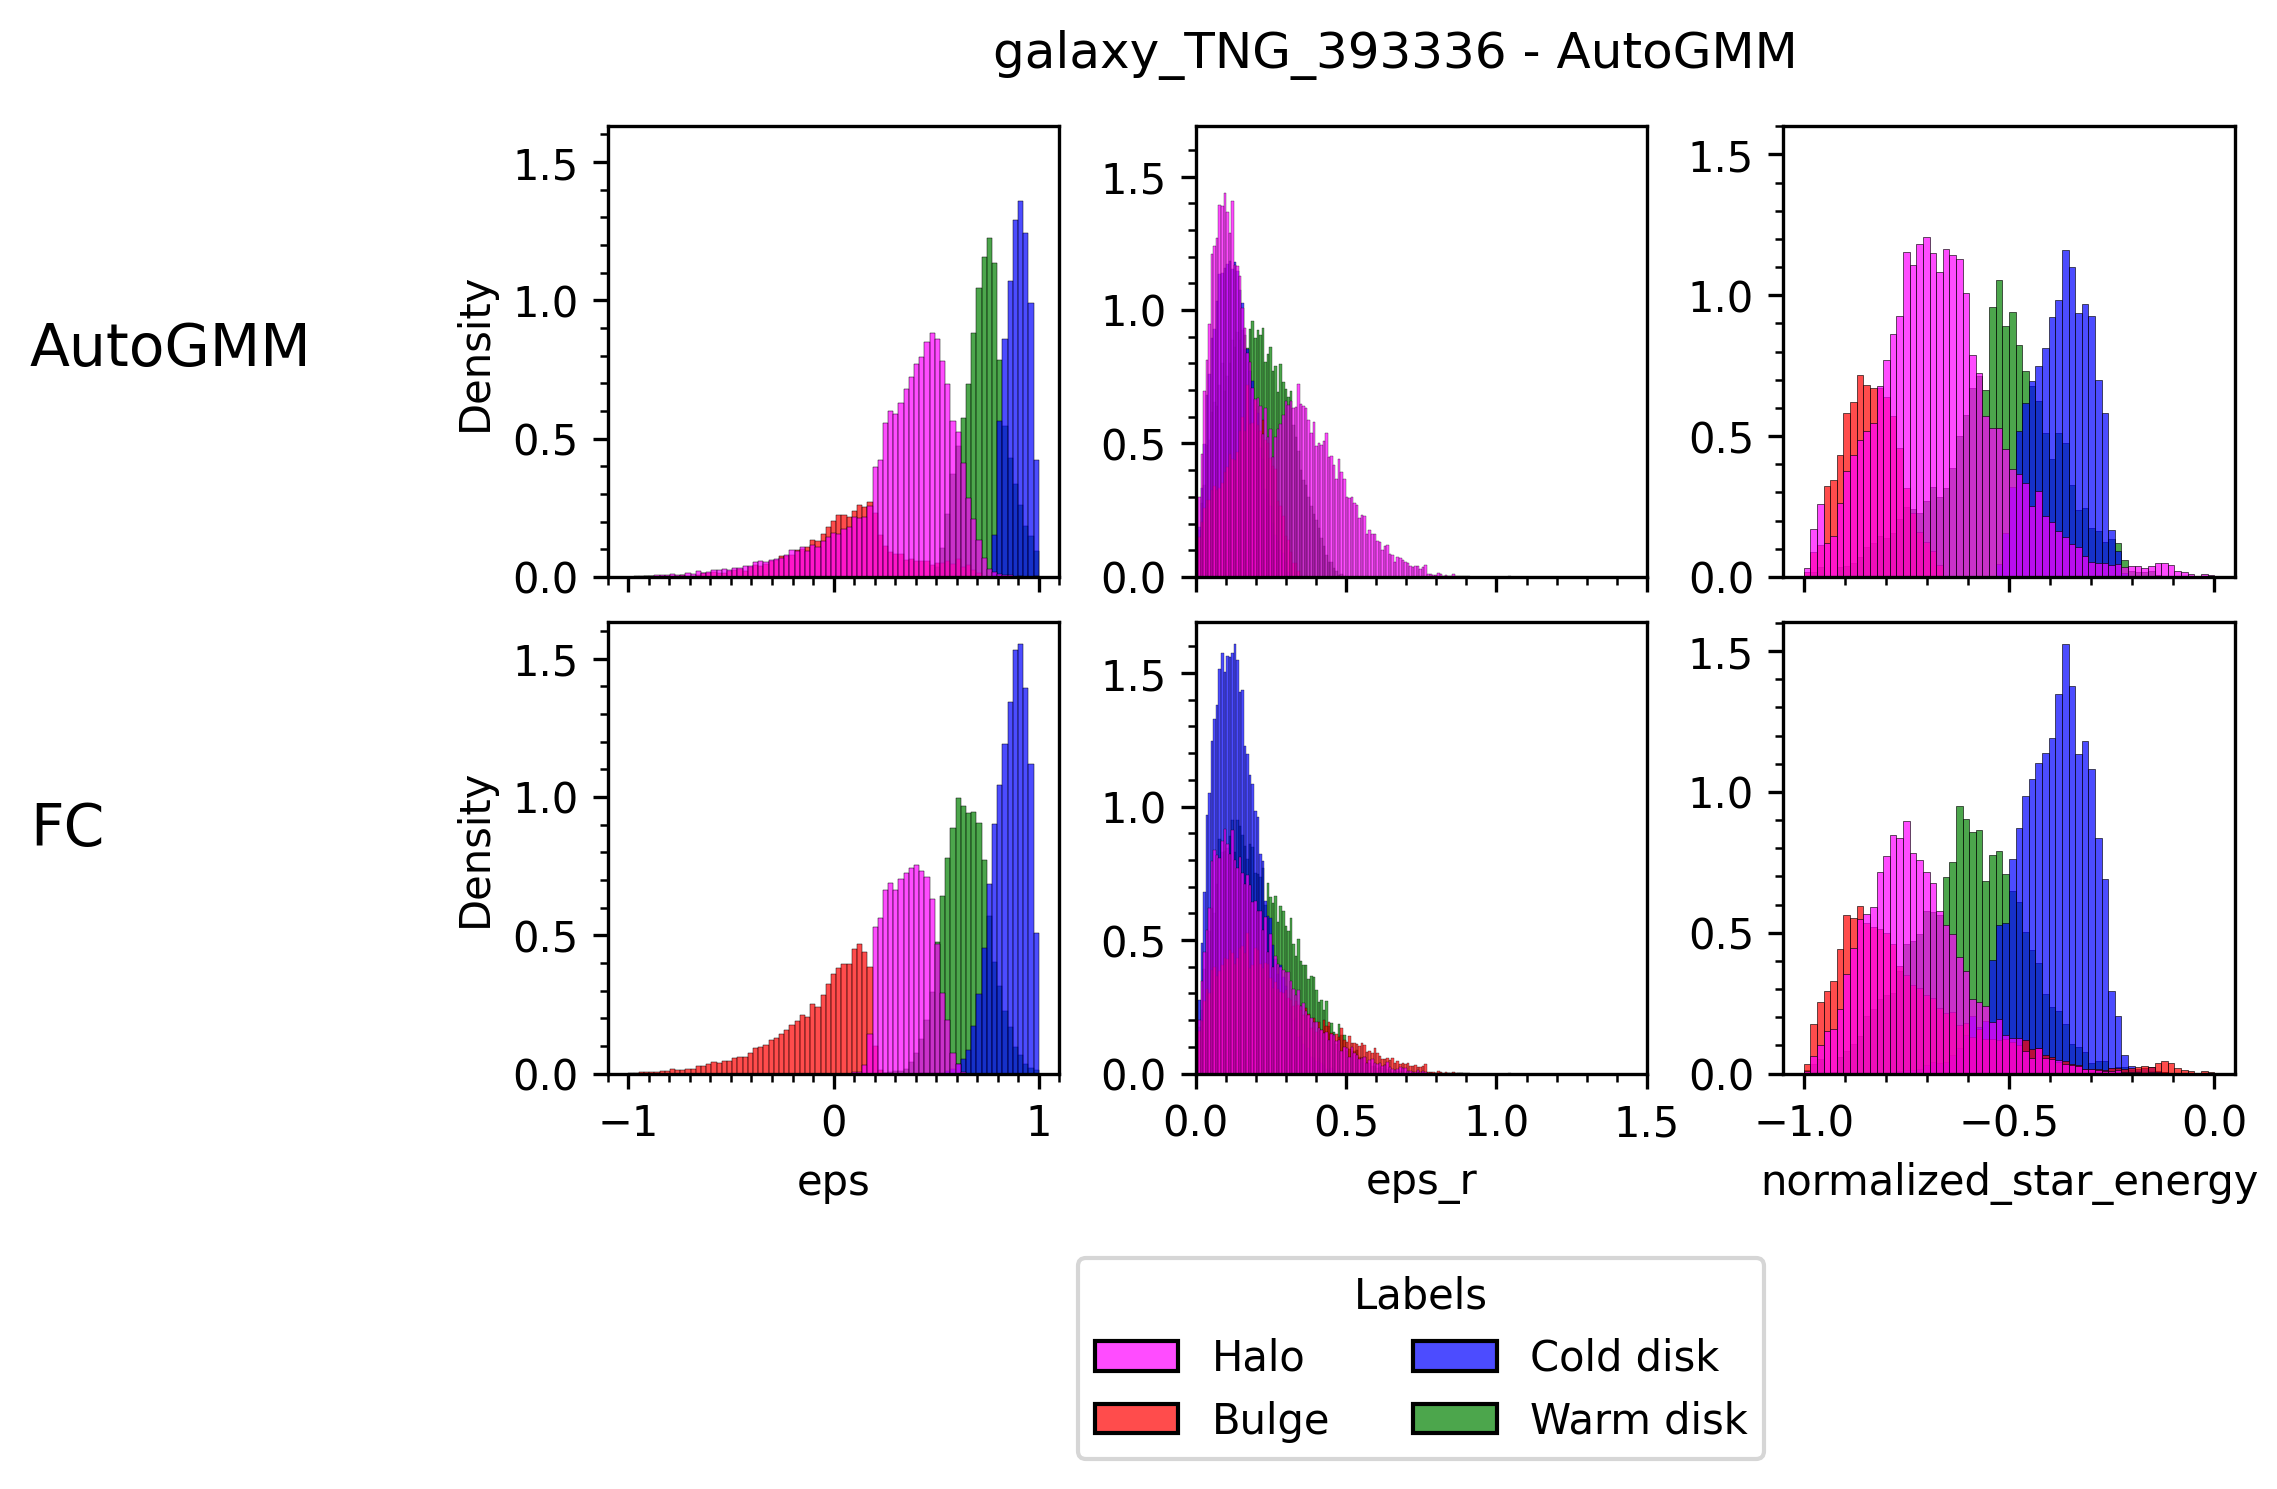
\includegraphics[width=7cm]{fuzzy clustering/figures/galaxy_TNG_393336 - circ histogram.png}
\end{center}

\vspace{-1cm}


\begin{table}
\centering
\begin{tabular}{l|c|c|c|c|}
\cline{3-5}
\multicolumn{2}{c|}{}&center.eps&center.eps\_r&center.normalized\_star\_energy\\
\cline{2-5}
& Bulge & $0.005$ & $0.229$ & $-0.764$\\
\cline{2-5}
& Halo & $0.368$ & $0.197$ & $-0.713$\\
\cline{2-5}
& Warm Disk & $0.632$ & $0.206$ & $-0.586$\\
\cline{2-5}
& Cold Disk & $0.857$ & $0.145$ & $-0.399$\\
\cline{2-5}
\end{tabular}
\end{table}

\note{
- FCM rapida transicion entre Bulge y Halo, por la poca distancia de los centros de cada cluster en normalized\_star\_energy en FCM. Entonces el peso que tendrán las distancias sobre esta feature a cada centro para calcular el valor de pertenencia de la partícula a cada cluster será similar entre ellas \\
- Si miramos la grafica tambien hay una tendencia sobreestimar el Cold Disk por sobre el Warm Disk\\
- Como sus centros en normalized star energy estan un tanto separados va a haber solapamiento entre ambos en eps.\\
- dos zonas de solapamiento, la que warm disk es mayor y la que cold disk es mayor. En la primera, el corte en AGMM es mas recto, por lo cual al tener mas fuzzines con FCM implica que varias particulas estelares van a estar en el Disco fino en lugar del grueso. Y en la segunda zona AGMM se solapa mas que FCM, por lo que sucede lo mismo, y colabora a que tenga mas densidad el Cold Disk. \\
- Este comportamiento se puede ver en la mayoria de las galaxias de nuestro dataset.
}

\end{frame}
\fi



\iflong
\begin{frame}
\frametitle{AGMM: Eliminación de outliers}
% 
% 

\begin{center}
    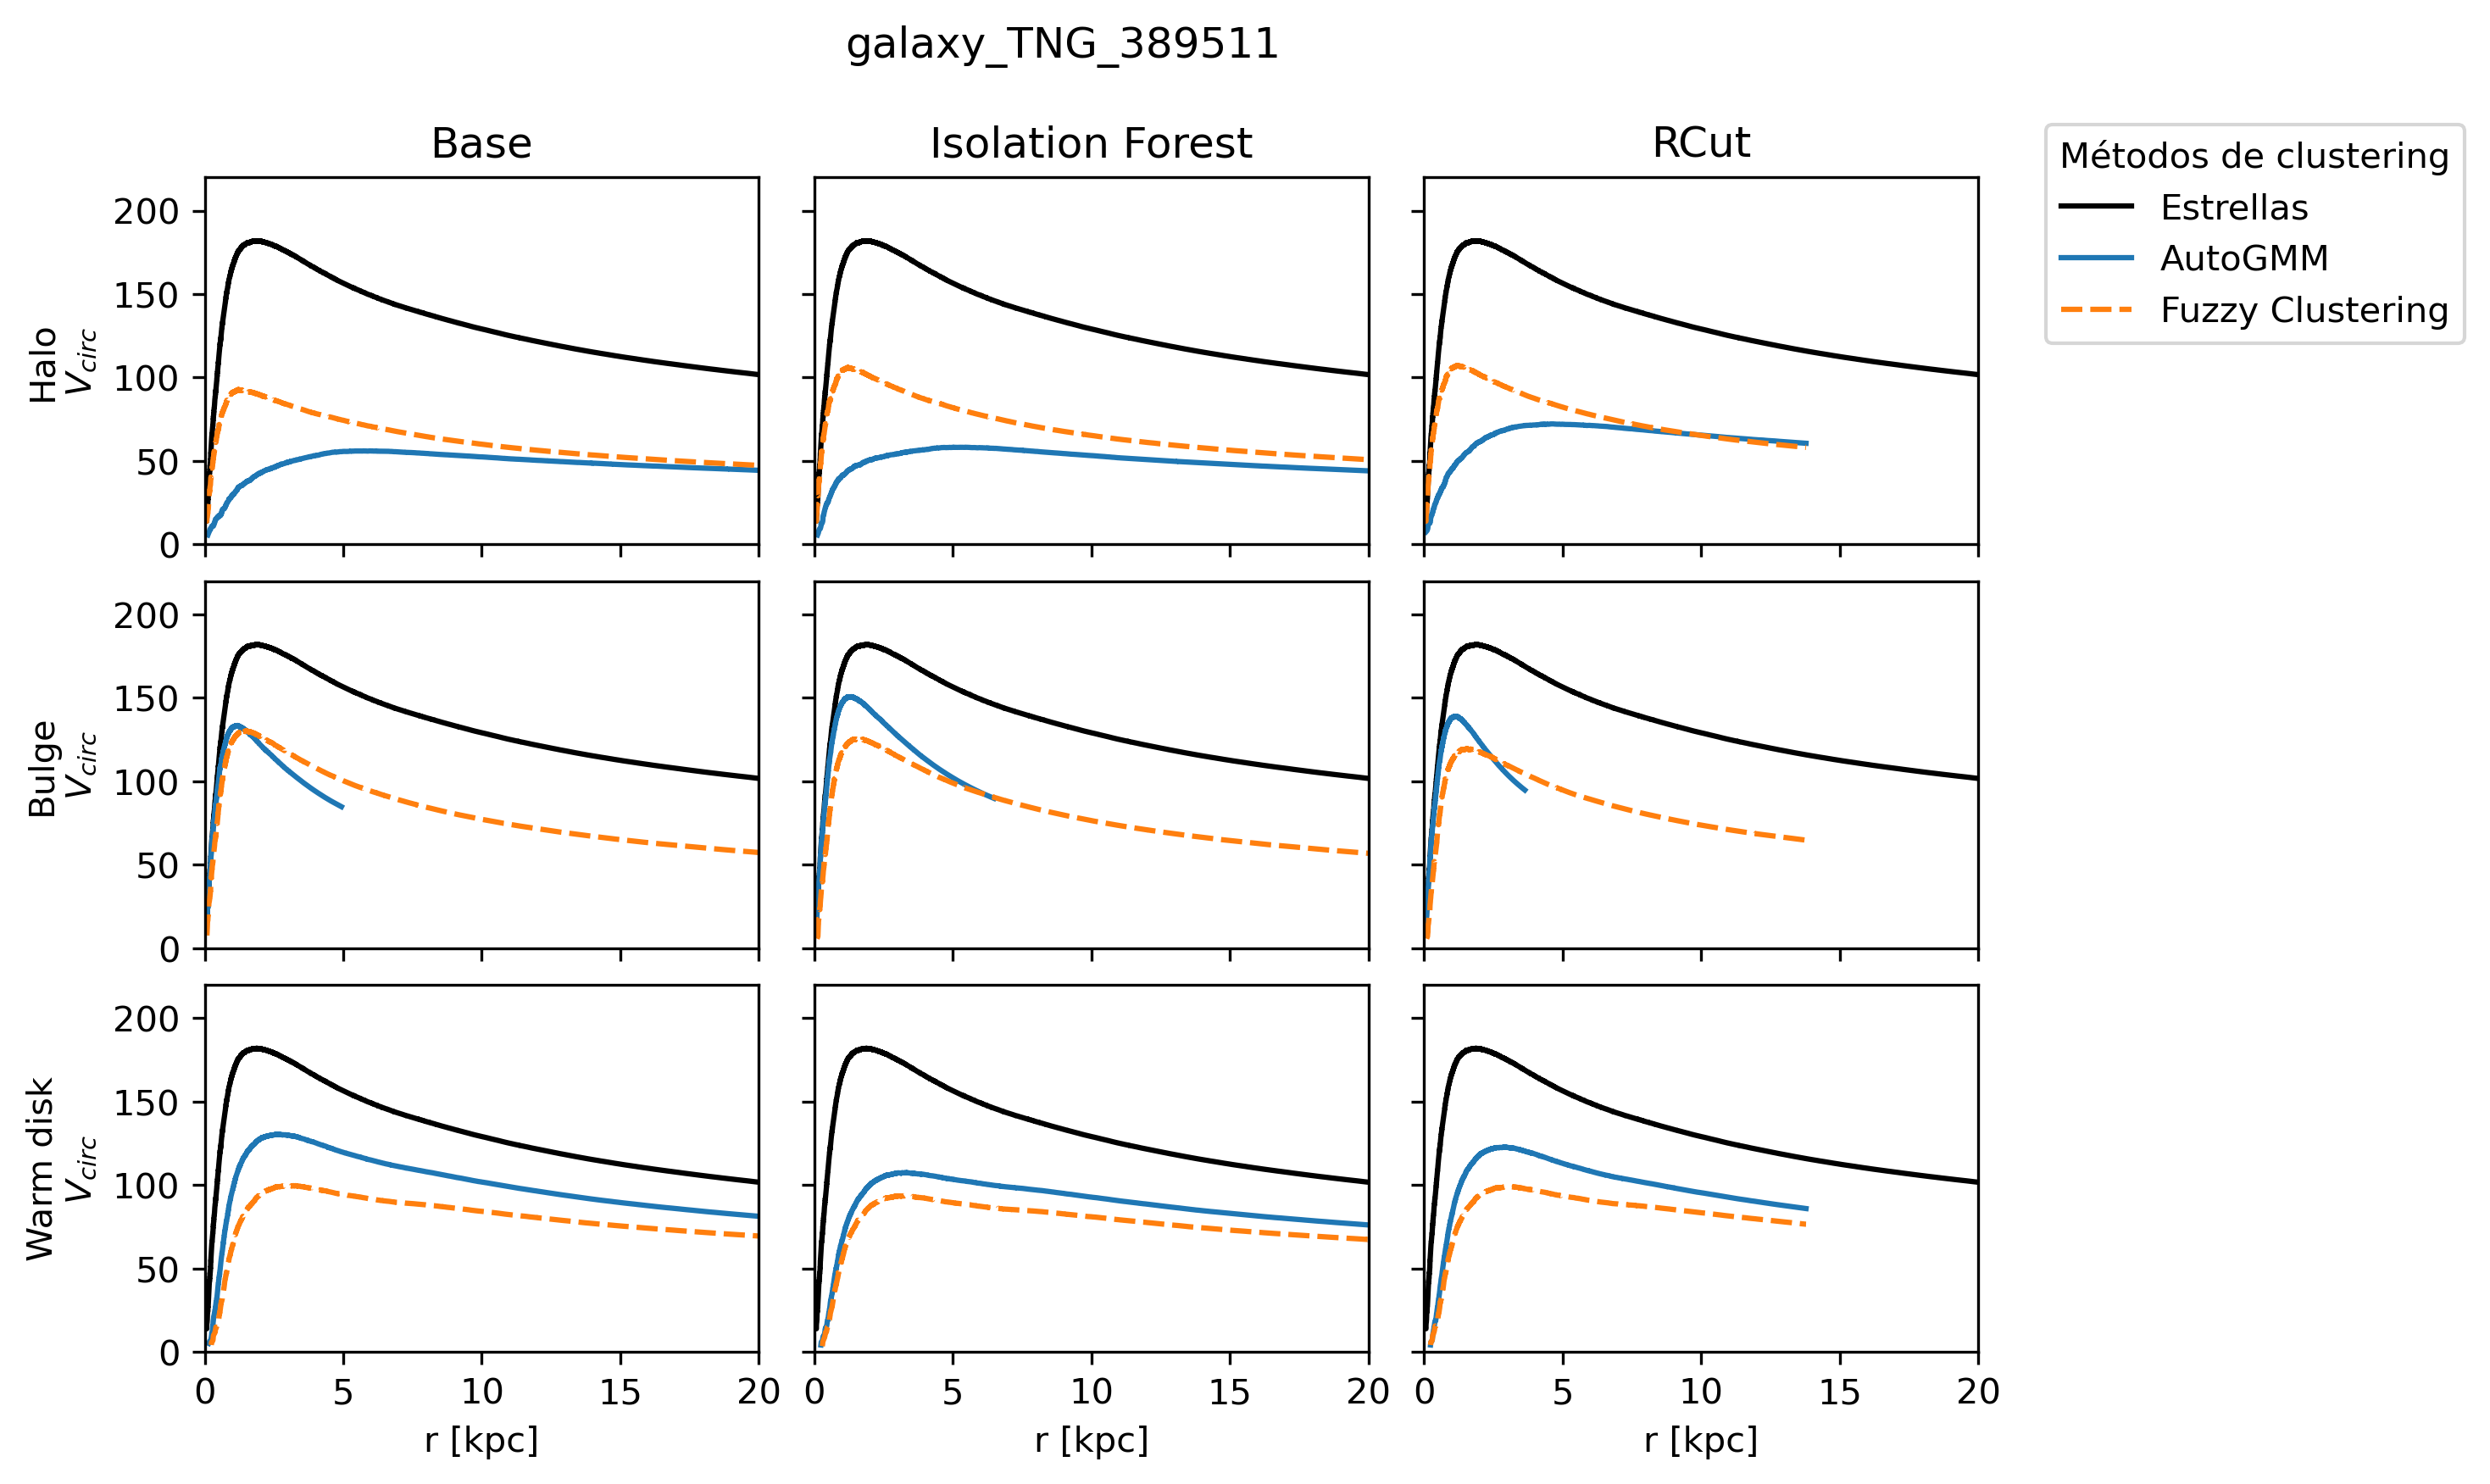
\includegraphics[width=12cm]{fuzzy clustering/figures/galaxy_TNG_389511 - AutoGMM - circ_velocity.png}
\end{center}

\note{
- Eliminar outliers en agmm tiene el mismo problema mencionado en la seccion anterior (n componentes) \\
- al igual que en la seccion anterior, tampoco obtuvimos diferencias tangibles al remover outliers dada la robustez del metodo
}

\end{frame}
\fi



\begin{frame}
\frametitle{AGMM: Eliminación de outliers}


\begin{columns}
\column{0.5\textwidth}

\begin{center}
    Promedio: 0.698
    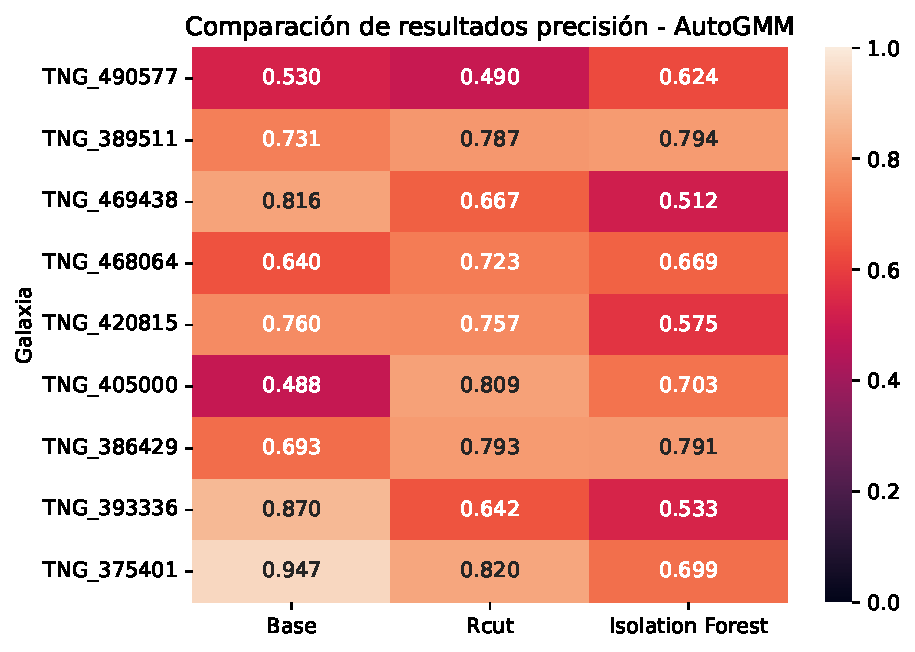
\includegraphics[width=6cm]{clustering jerarquico/figures/precision - agmm.pdf}
\end{center}
\column{0.5\textwidth}
\begin{center}
    Promedio: 0.626
    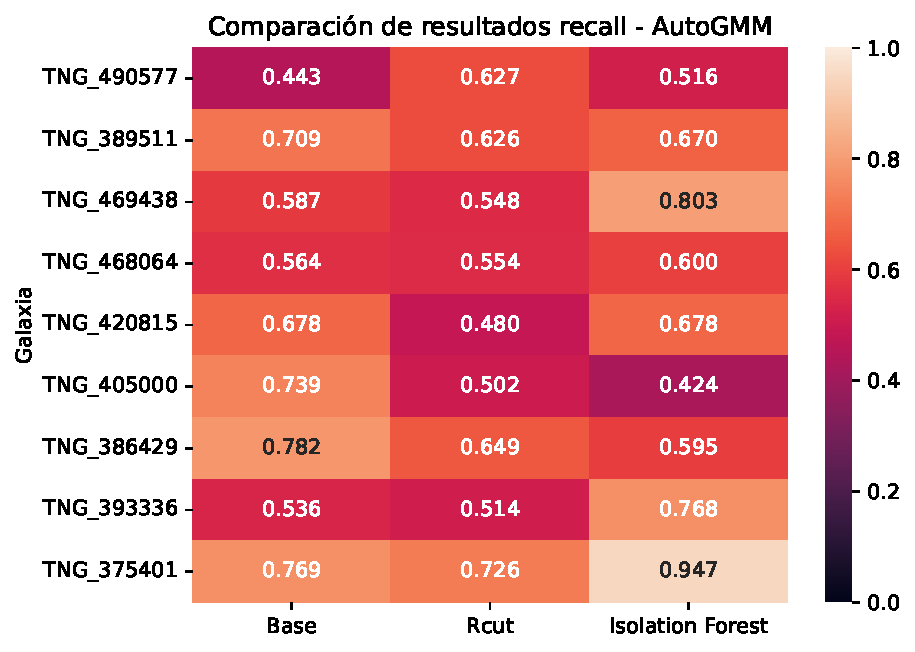
\includegraphics[width=6cm]{clustering jerarquico/figures/recall - agmm.pdf}
\end{center}
\end{columns}

\note{
%- Eliminar outliers en agmm tiene el mismo problema mencionado en la seccion anterior (n componentes) \\
- al igual que en la seccion anterior, tampoco obtuvimos diferencias tangibles al remover outliers dada la \textbf{robustez del metodo} \\
- \textbf{No es una buena alternativa de agmm}
}


\end{frame}




\section{Evidence Accumulation Clustering}

\begin{frame}
\frametitle{Evidence Accumulation Clustering}

\begin{center}
    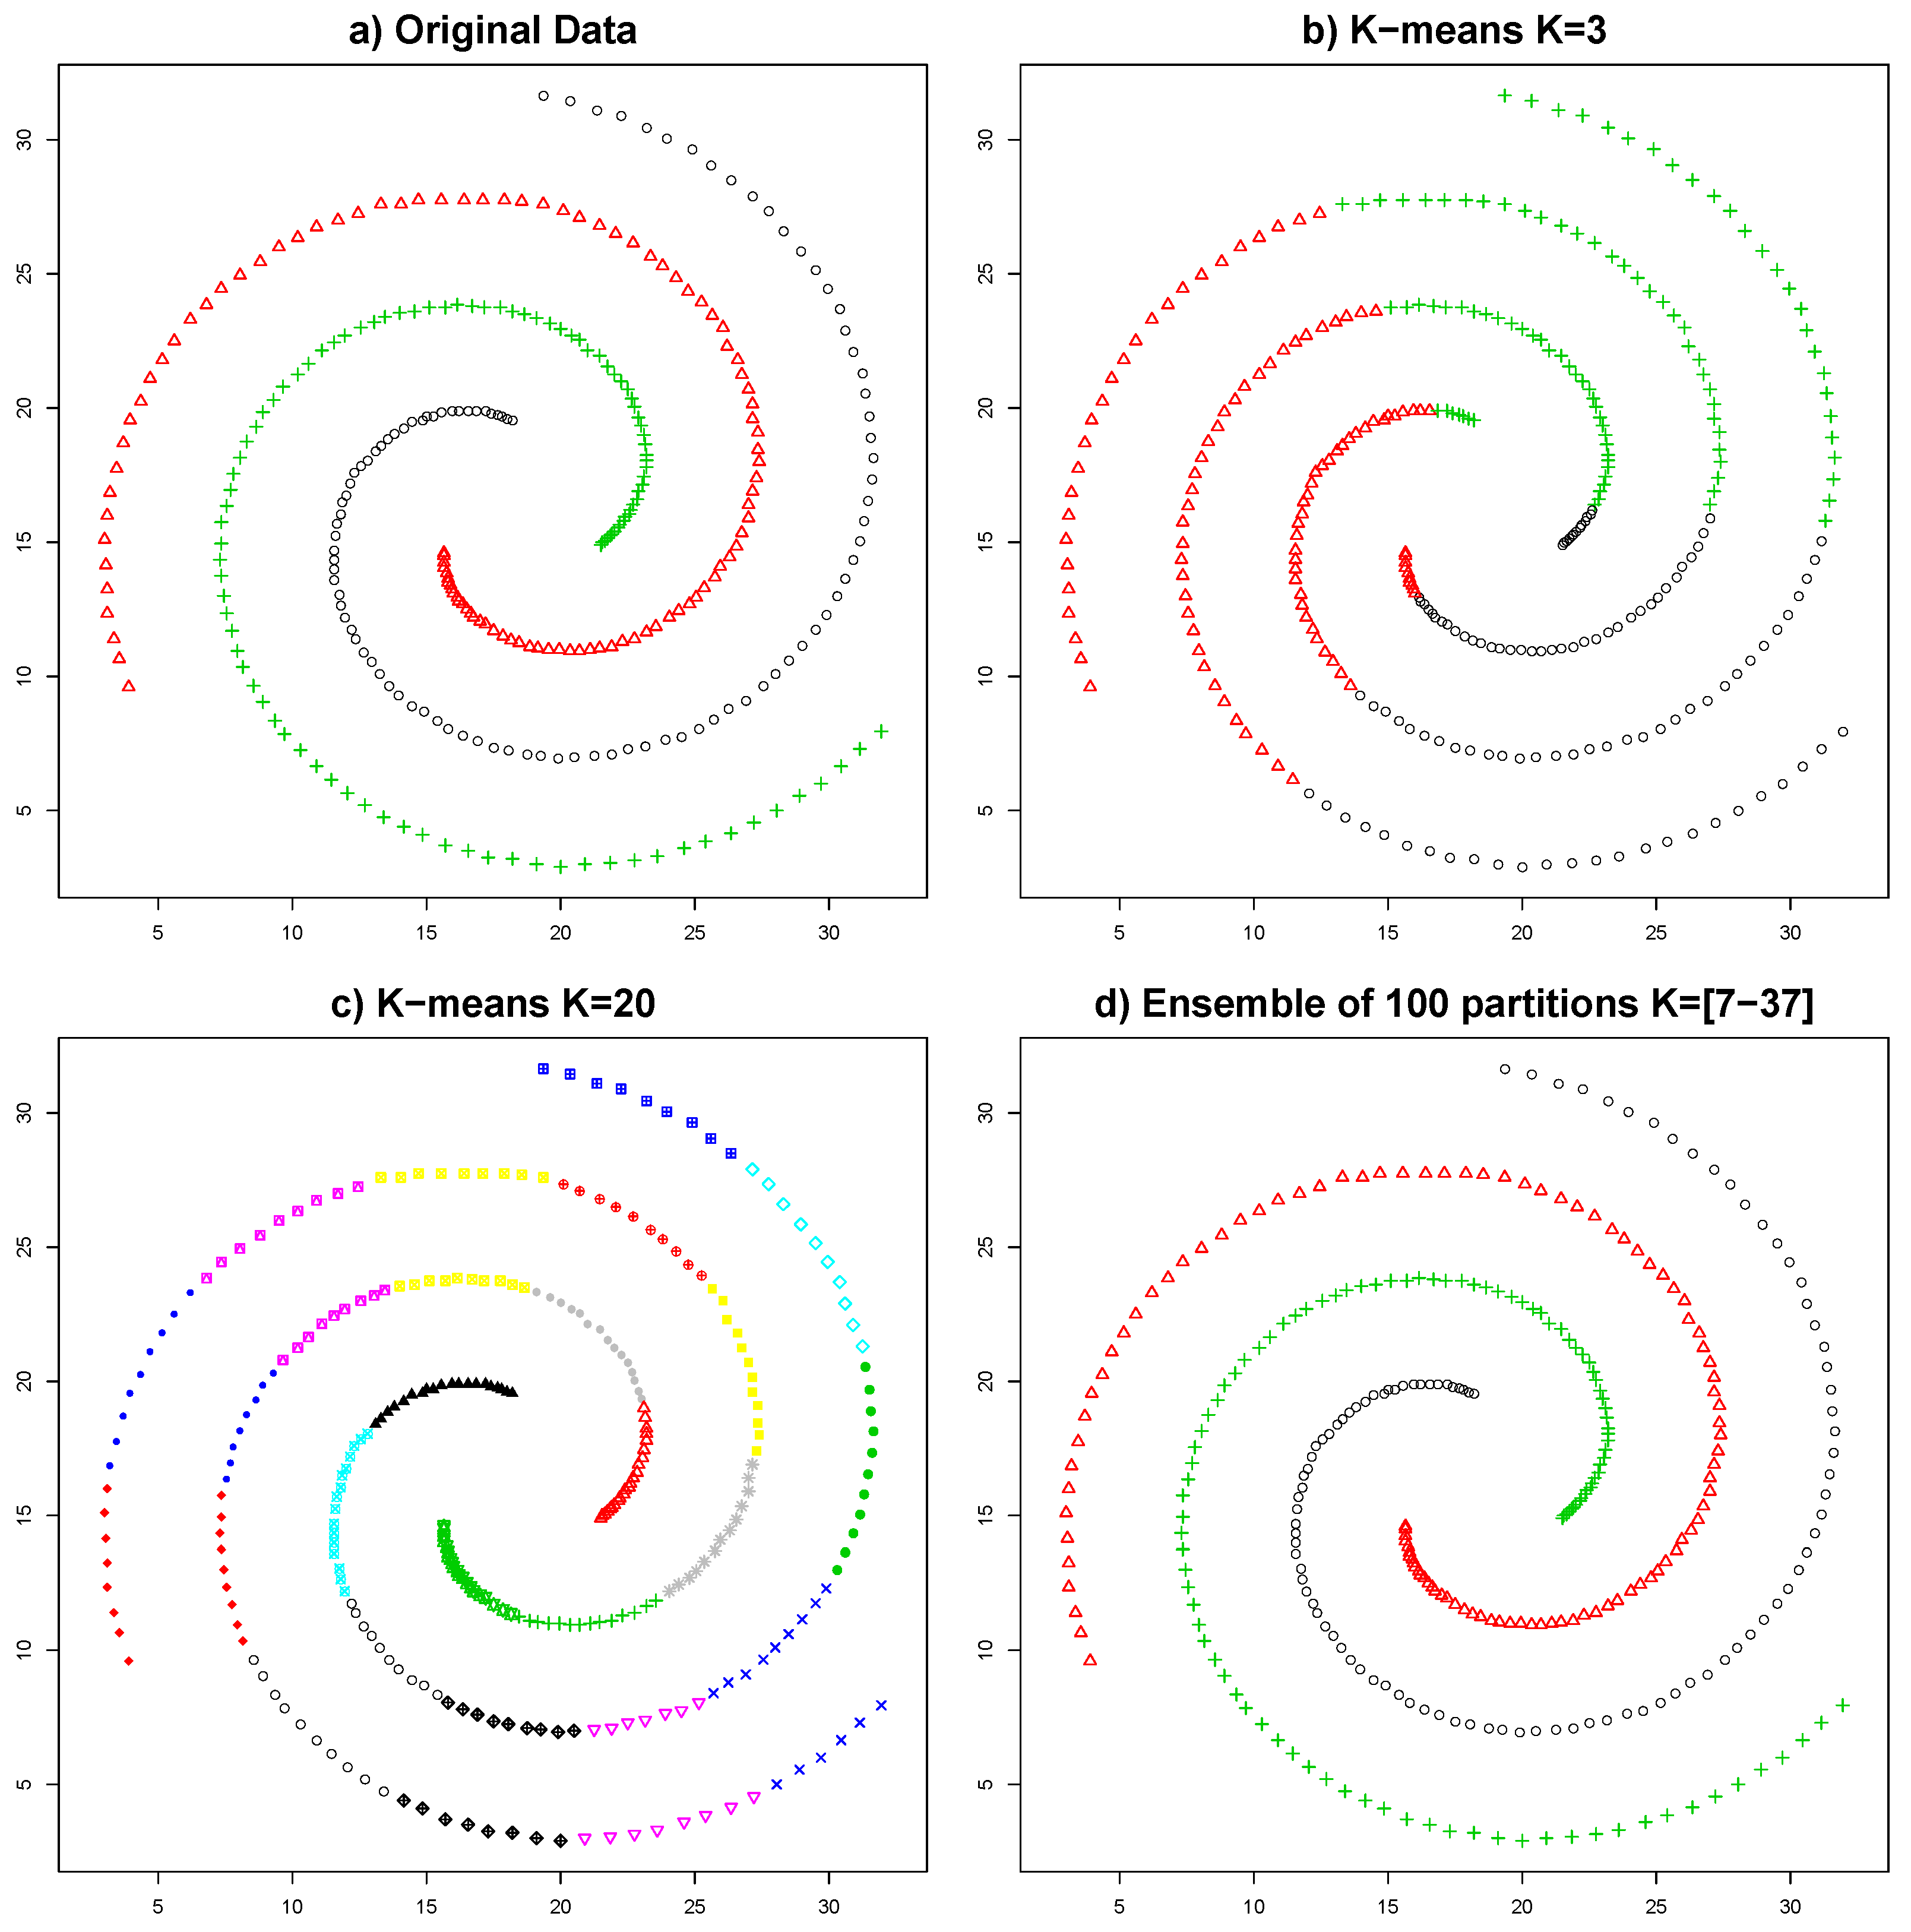
\includegraphics[width=7cm]{evidence accumulation clustering/figures/ensamble-example.png}
\end{center}

\note{
- Los métodos de clustering ensambles se basan en tomar \textbf{resultados} generados por \textbf{múltiples algoritmos} de clustering y llegar a un \textbf{consenso} que sea más correcto que los resultados individuales de los algoritmos utilizados. \\ %EAC es uno de ellos, y vamos a estar utilizandolo en esta ultima seccion. \\
- La idea detrás de \gls{EAC} es entonces \textbf{combinar los resultados de múltiples} clusterings en una \textbf{única partición de datos}, interpretando cada uno de estos resultados como una ``\textbf{evidencia independiente}'' de la organización de los datos, como puede apreciarse en la figura
}

\end{frame}

\begin{frame}
\frametitle{Evidence Accumulation Clustering}

\begin{itemize}
    \item<1-> Sea $X = {x_1, x_2,...,x_n}$ nuestro conjunto de datos donde $x_i \in R^d$ y $R^d$ es un espacio de $d$ features.
    \item<2-> Partición $P$ que encuentra $k$ clusters
    \item<3-> Dado $N$ algoritmos de clustering podemos entonces derivar $N$ particiones $P$
    \item<4-> Definimos al conjunto de estas particiones como:

    \begin{equation}
    \mathbb{P} = \{P^1, P^2,...,P^N\}
    \end{equation}
    
    \begin{multline}
    \hfill
        \begin{split}
        P^1 = \{C^1_1, C^1_2,...,C^1_{k_1}\}
        \end{split} \hfill \break
    \hdots \hfill \break
        \begin{split}
        P^N = \{C^N_1, C^N_2,...,C^N_{k_N}\}
        \end{split}
    \hfill
    \end{multline}

\note{
- \noindent donde $C^i_j$ es el cluster $j$th en la partición $P^i$, la cual tiene $k_i$ clusters. \\
- Además, dado $n^i_j$ como la cardinalidad de $C^i_j$, se cumple que $\sum_{j=1}^{k_i} n^i_j=n, \ \ i=1,...,N$. \\
- Cabe aclarar que los k pueden ser diferentes. \gls{EAC} no asume el número de clusters $k_i$ para cada partición obtenida $P^i$, por lo que cada $k_i$ pueden ser no sólo diferentes al número de clusters buscado por \gls{EAC}, sino que también entre sí.
}
\end{itemize}

\end{frame}

\iflong
\begin{frame}
\frametitle{Evidence Accumulation Clustering}

El objetivo es obtener una partición de datos ``óptima'' llamada $P^*$, que cumpla con las siguientes propiedades:
\begin{itemize}
    \item<1-> Consistencia con el ensamble de clusterings $\mathbb{P}$
    \item<2-> Robustez antes pequeñas variaciones en $\mathbb{P}$
    \item<3-> Ajuste con respecto al \gls{GT}
\end{itemize}

\note{
\begin{itemize}
    \item<1-> Significa que $\mathbb{P}$ sea el r\textbf{esultado de un acuerdo} entre las diferentes \textbf{partes encontradas} $P^i, i=1,...,N$.
    \item<2-> Los cantidad de clusters y los puntos pertenecientes a cada cluster en $P^*$ \textbf{deberían ser invariantes} ante \textbf{pequeñas perturbaciones} de $\mathbb{P}$.
    \item<3-> Los clusters encontrados deberán \textbf{coincidir} fuertemente con las \textbf{verdaderas etiquetas} de nuestros datos.
\end{itemize}
}

\end{frame}
\fi








\begin{frame}
\frametitle{Evidence Accumulation Clustering}

Tres problemas a resolver, que definen cada etapa del algoritmo de \gls{EAC}:

\begin{enumerate}
    \item  Cómo generamos el ensamble de particiones.
    \item  Cómo combinamos la evidencia.
    \item  Cómo extraemos una partición de datos (conjunto de clusters) consistente de la evidencia combinada.
\end{enumerate}

\note{
- Utilizaremos un algoritmo en particular, \textbf{k-means}, múltiples veces con \textbf{semillas diferentes} para generar el ensamble de clusters. \\
%- Para quienes no esten familiarizados con k-means es un algoritmo clásico del área de minería de datos. Dado un conjunto de k clusters buscados, asigna de forma aleatoria los centros de dichos clusters y los optimmiza iterativamente, asignando los puntos al centro del cluster más cercano en cada iteración. Similar Fuzzy clustering que explicamos antes. \\
%- Como el algoritmo es naturalmente inestable significa que podemos utilizar la variabilidad de múltiples corridas de k-means para llegar a un consenso, como se propone realizar con \gls{EAC}.
}

\end{frame}


\iflong
\begin{frame}
\frametitle{Evidence Accumulation Clustering}

El primer problema se puede abordar de las siguientes maneras:

\begin{enumerate}
\item<1-> Elección de representación de datos:
    \begin{enumerate}
     \item<2-> Empleando diferentes métodos de preprocesamiento y/o extracción de features.
     % , lo que resulta en diferentes representaciones de los datos o espacio de features.
     \item<3-> Explorando subespacios de la misma representación de datos.
     \item<4-> Perturbando los datos con métodos de bootstrapping o sampling.
     \end{enumerate}
\item<5-> Elección de algoritmos de clustering o parámetros de los algoritmos:
    \begin{enumerate}
     \item<6-> Aplicando diferentes algoritmos de clustering.
     \item<7-> Usando el mismo algoritmo pero con diferentes parámetros o inicializaciones.
     \item<8-> Explorando diferentes medidas de disimilitud para evaluar relaciones en nuestros datos.
     \end{enumerate}
\end{enumerate}

\note{
- Dos categorias sobre como resolver el problema. \\
- En este trabajo nos interesara aplicar lo mencionado en 2)b). Es decir, utilizaremos un algoritmo en particular, k-means, múltiples veces con semillas diferentes para generar el ensamble de clusters. \\
- Para quienes no esten familiarizados con k-means es un algoritmo clásico del área de minería de datos. Dado un conjunto de k clusters buscados, asigna de forma aleatoria los centros de dichos clusters y los optimmiza iterativamente, asignando los puntos al centro del cluster más cercano en cada iteración. Similar Fuzzy clustering que explicamos antes. \\
- Como el algoritmo es naturalmente inestable significa que podemos utilizar la variabilidad de múltiples corridas de k-means para llegar a un consenso, como se propone realizar con \gls{EAC}.
}

\end{frame}
\fi




\begin{frame}
\frametitle{Evidence Accumulation Clustering}

\begin{center}
    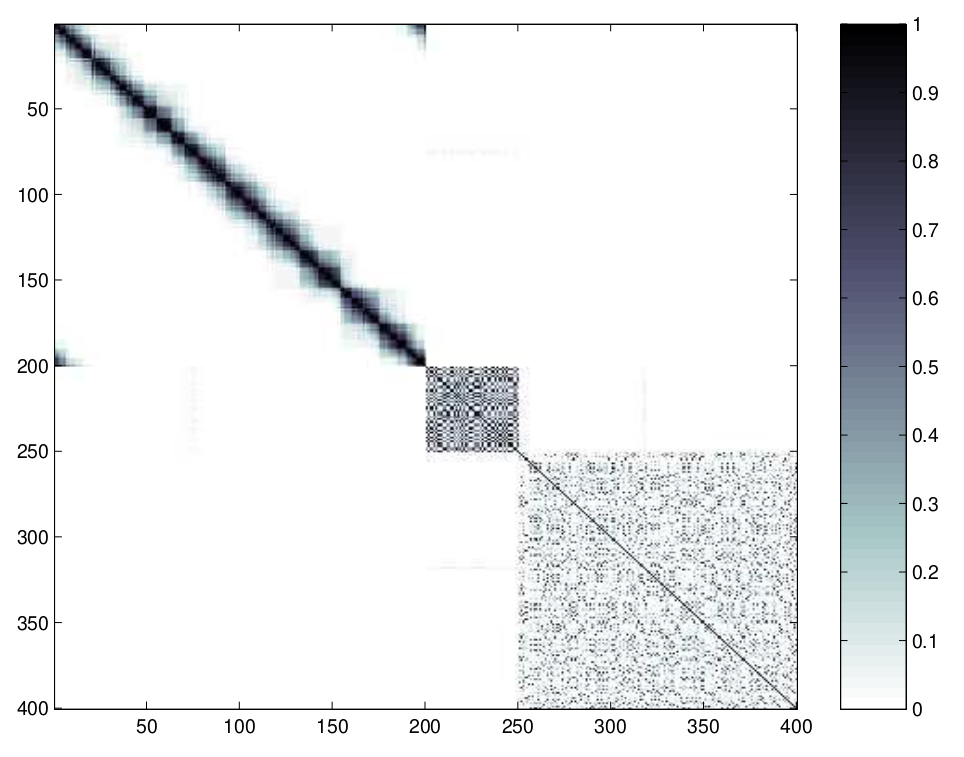
\includegraphics[width=6cm]{evidence accumulation clustering/figures/co-association matrix.png}
\end{center}

Mecanismo de votación y métrica de similitud

$$
C(i,j) = \frac{n_{ij}}{N}
$$

Donde $n_{ij}$ es el número de veces que el par de puntos $(i,j)$ son asignados al mismo cluster en $N$ particiones.

\note{
- Una vez obtenido el ensamble de particiones, pasaremos a combinar la información proveída de estos con una \textbf{matriz de co-asociación}. Esta nos permitirá \textbf{relacionar la información obtenida} con cada partición incluso si la cardinalidad varía entre ellas. \\
- Bajo la suposición de que dos puntos \textbf{pertenecen al mismo cluster} si se encontraron \textbf{en el mismo cluster repetidas veces} en el ensamble de particiones \\
- Una vez generada la \textbf{matriz de similitud} podemos aplicar \textbf{cualquier algoritmo de clustering sobre ésta}. El paper original opta por utilizar \textbf{clustering jerárquico aglomerativo} con \textbf{single o average} linkage, por lo que seguimos con eso.
}

\end{frame}


\begin{frame}
\frametitle{Librería utilizada}

\begin{center}

\href{https://pycombo.readthedocs.io/en/latest/}{https://pycombo.readthedocs.io/en/latest/}
\href{https://github.com/originalnicodr/combo}{https://github.com/originalnicodr/combo}

\end{center}

\note{
%- Aunque el paper original describe cómo la elección de donde cortar el dendrograma se realiza a partir de una medida de ``tiempo'' respecto a qué tanto se mantienen los clusters en el dendrograma antes de juntarse con otro, la librería mencionada nos da la opción de cortar el dendrograma en donde queramos para así obtener una partición de nuestros datos con la cantidad específica de clusters que buscamos. Esto nos es de especial utilidad para realizar los experimentos y comparaciones que venimos haciendo en los capítulos anteriores.\\
- Porque forkeamos la libreria 
}

\end{frame}


\begin{frame}
\frametitle{Abadi: Detección de 2 componentes}


\begin{columns}
\column{0.4\textwidth}
\begin{center}
\begin{itemize}
 \item $N = 500$
 \item k-means con $k_i = 100, i = 1, ..., N$.
\item Clustering Jerárquico aglomerativo con single linkage
\end{itemize}
\end{center}
\column{0.6\textwidth}
    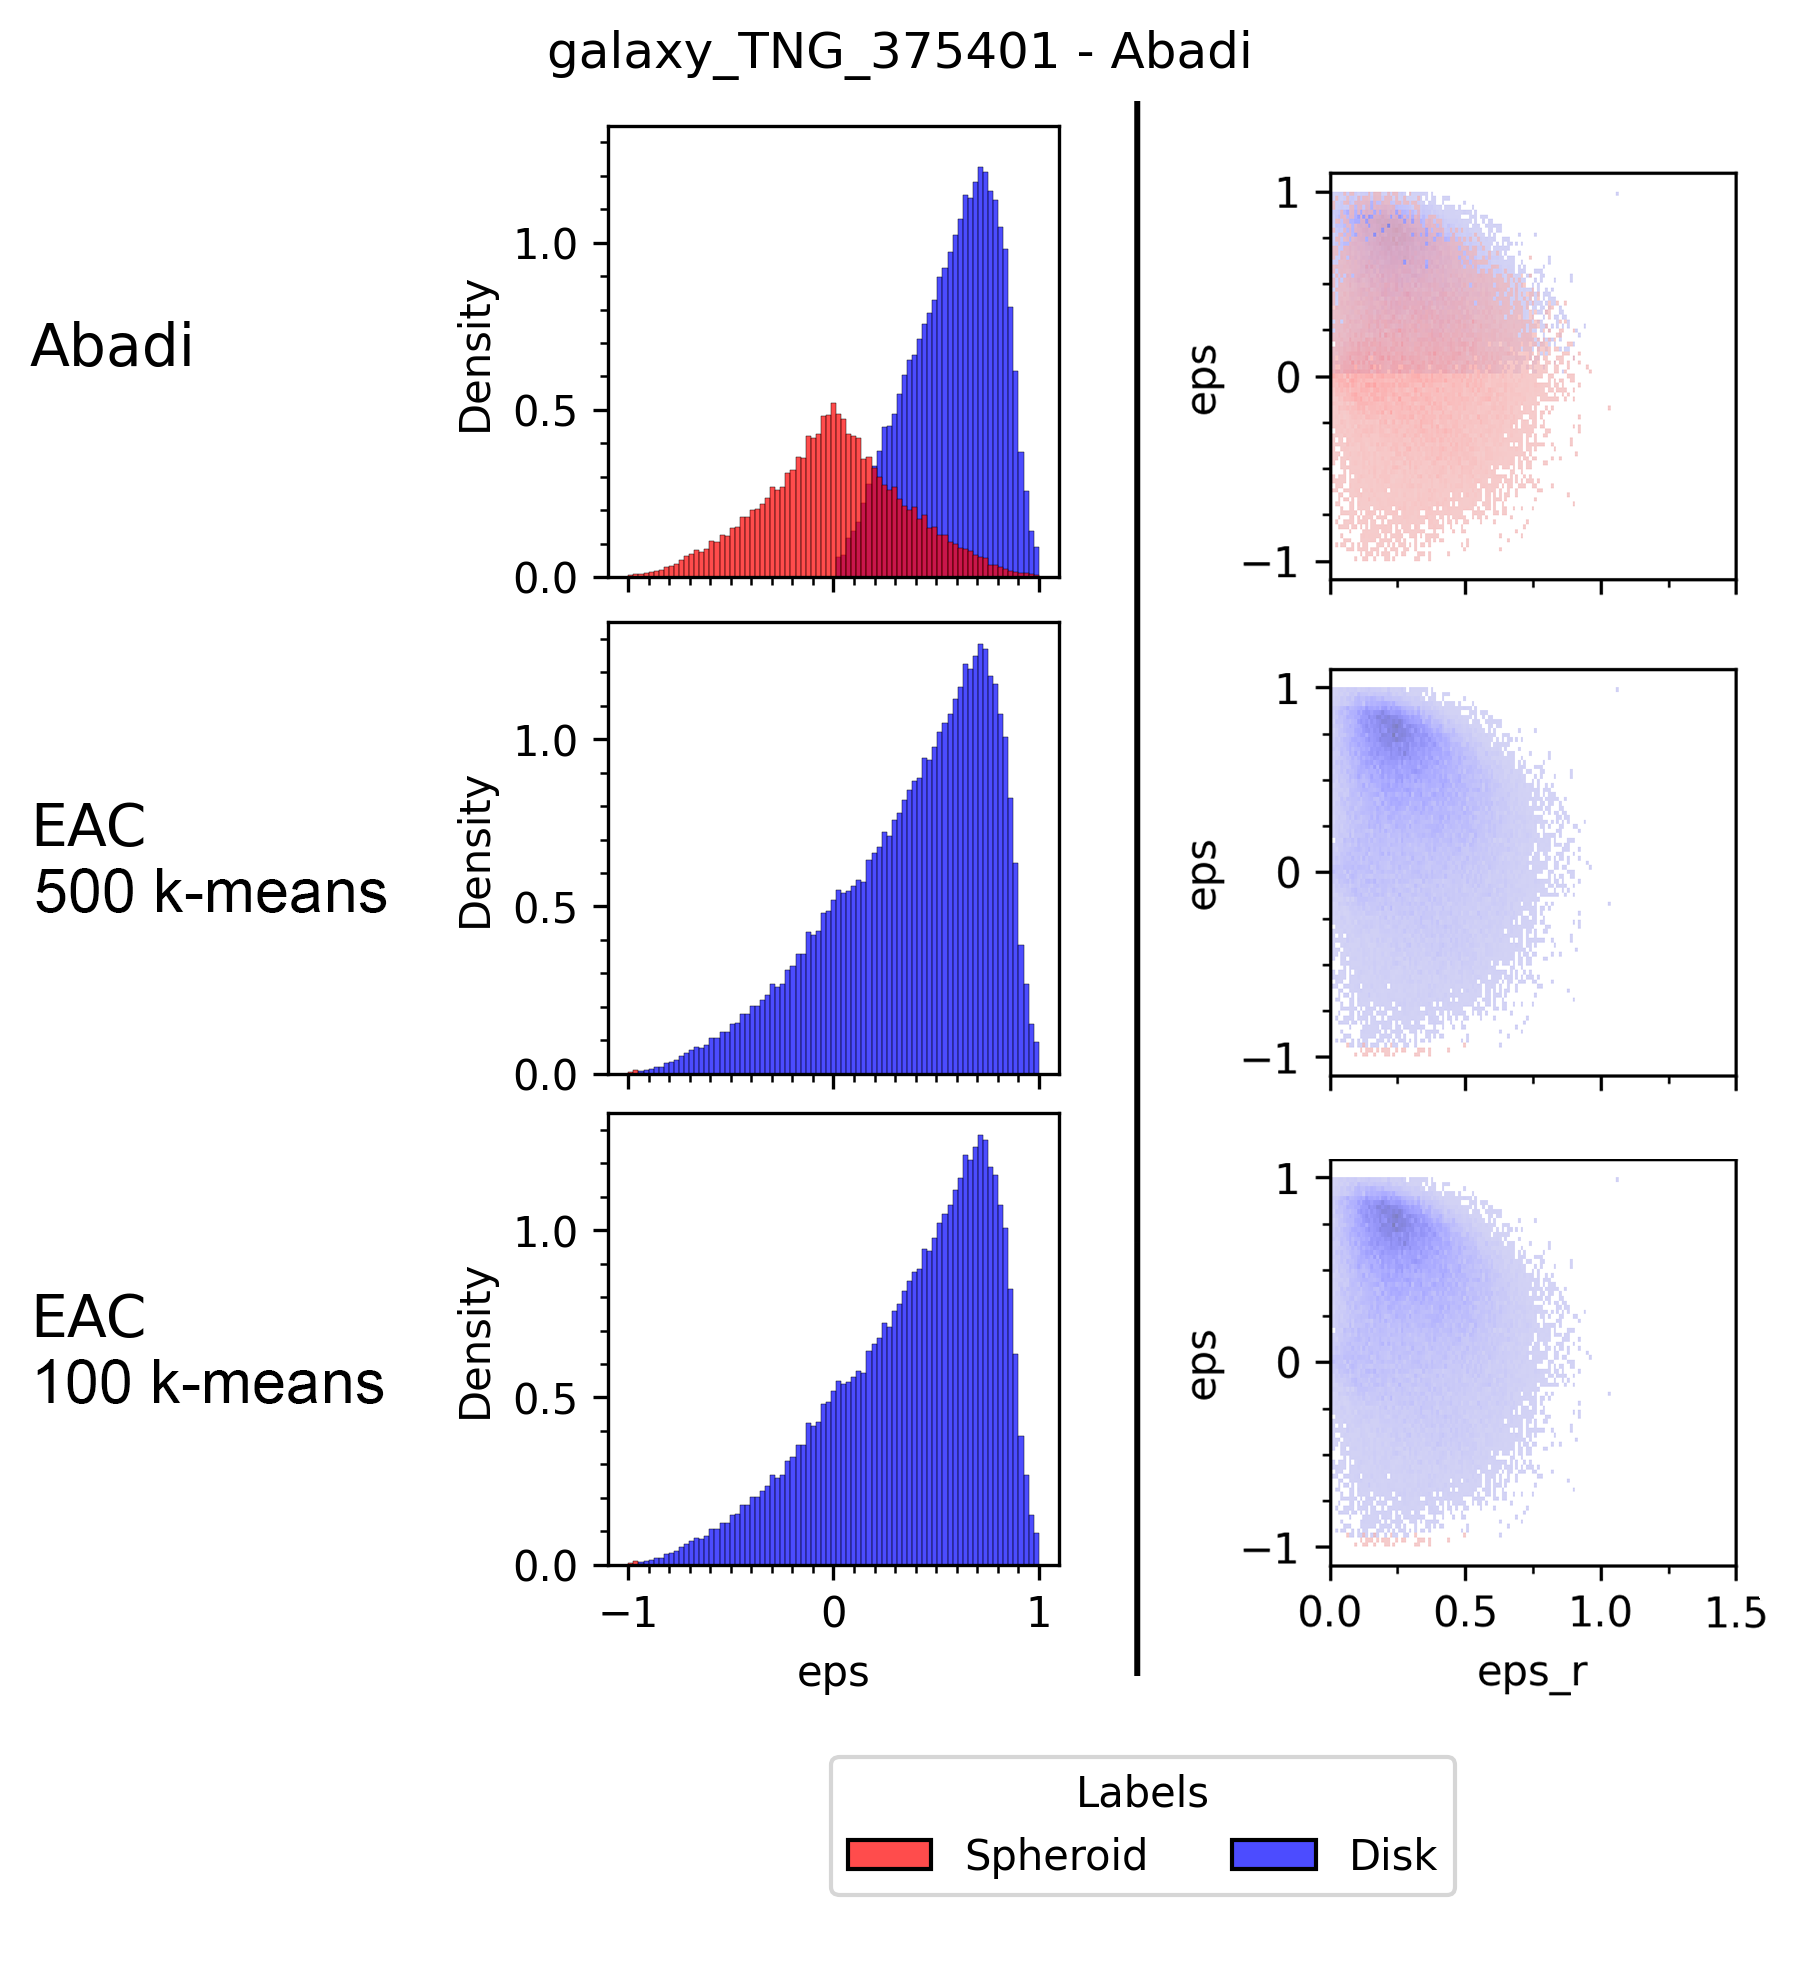
\includegraphics[width=6cm]{evidence accumulation clustering/figures/eac kmeans 500 vs 100.png}
\end{columns}

\note{
-  Habiamos probado con N = 500, pero \textbf{tardaba aun mas (cuatro dias)}, por lo cual optamos por reducir el numero de particiones a buscar a 100 \\
- La diferencia con N=500 era casi \textbf{imperciptible} \\
- Pero sigue siendo muy \textbf{caro computacionalmente}, por eso redujimos el analisis a tan solo \textbf{tres galaxias}, y dado los resultados feos que estamos viendo no valia la pena probarlos con todas (la falta de galaxias no es de gran impacto para nuestro analisis) \\
- \textbf{Por que da asi?} Antes de explicar: %Primero tenemos que ver la pinta que tienen los resultados de k-means (siguiente diapo)\\
}

\end{frame}


 \iflong
\begin{frame}
\frametitle{Abadi: Detección de 2 componentes}

\begin{center}
    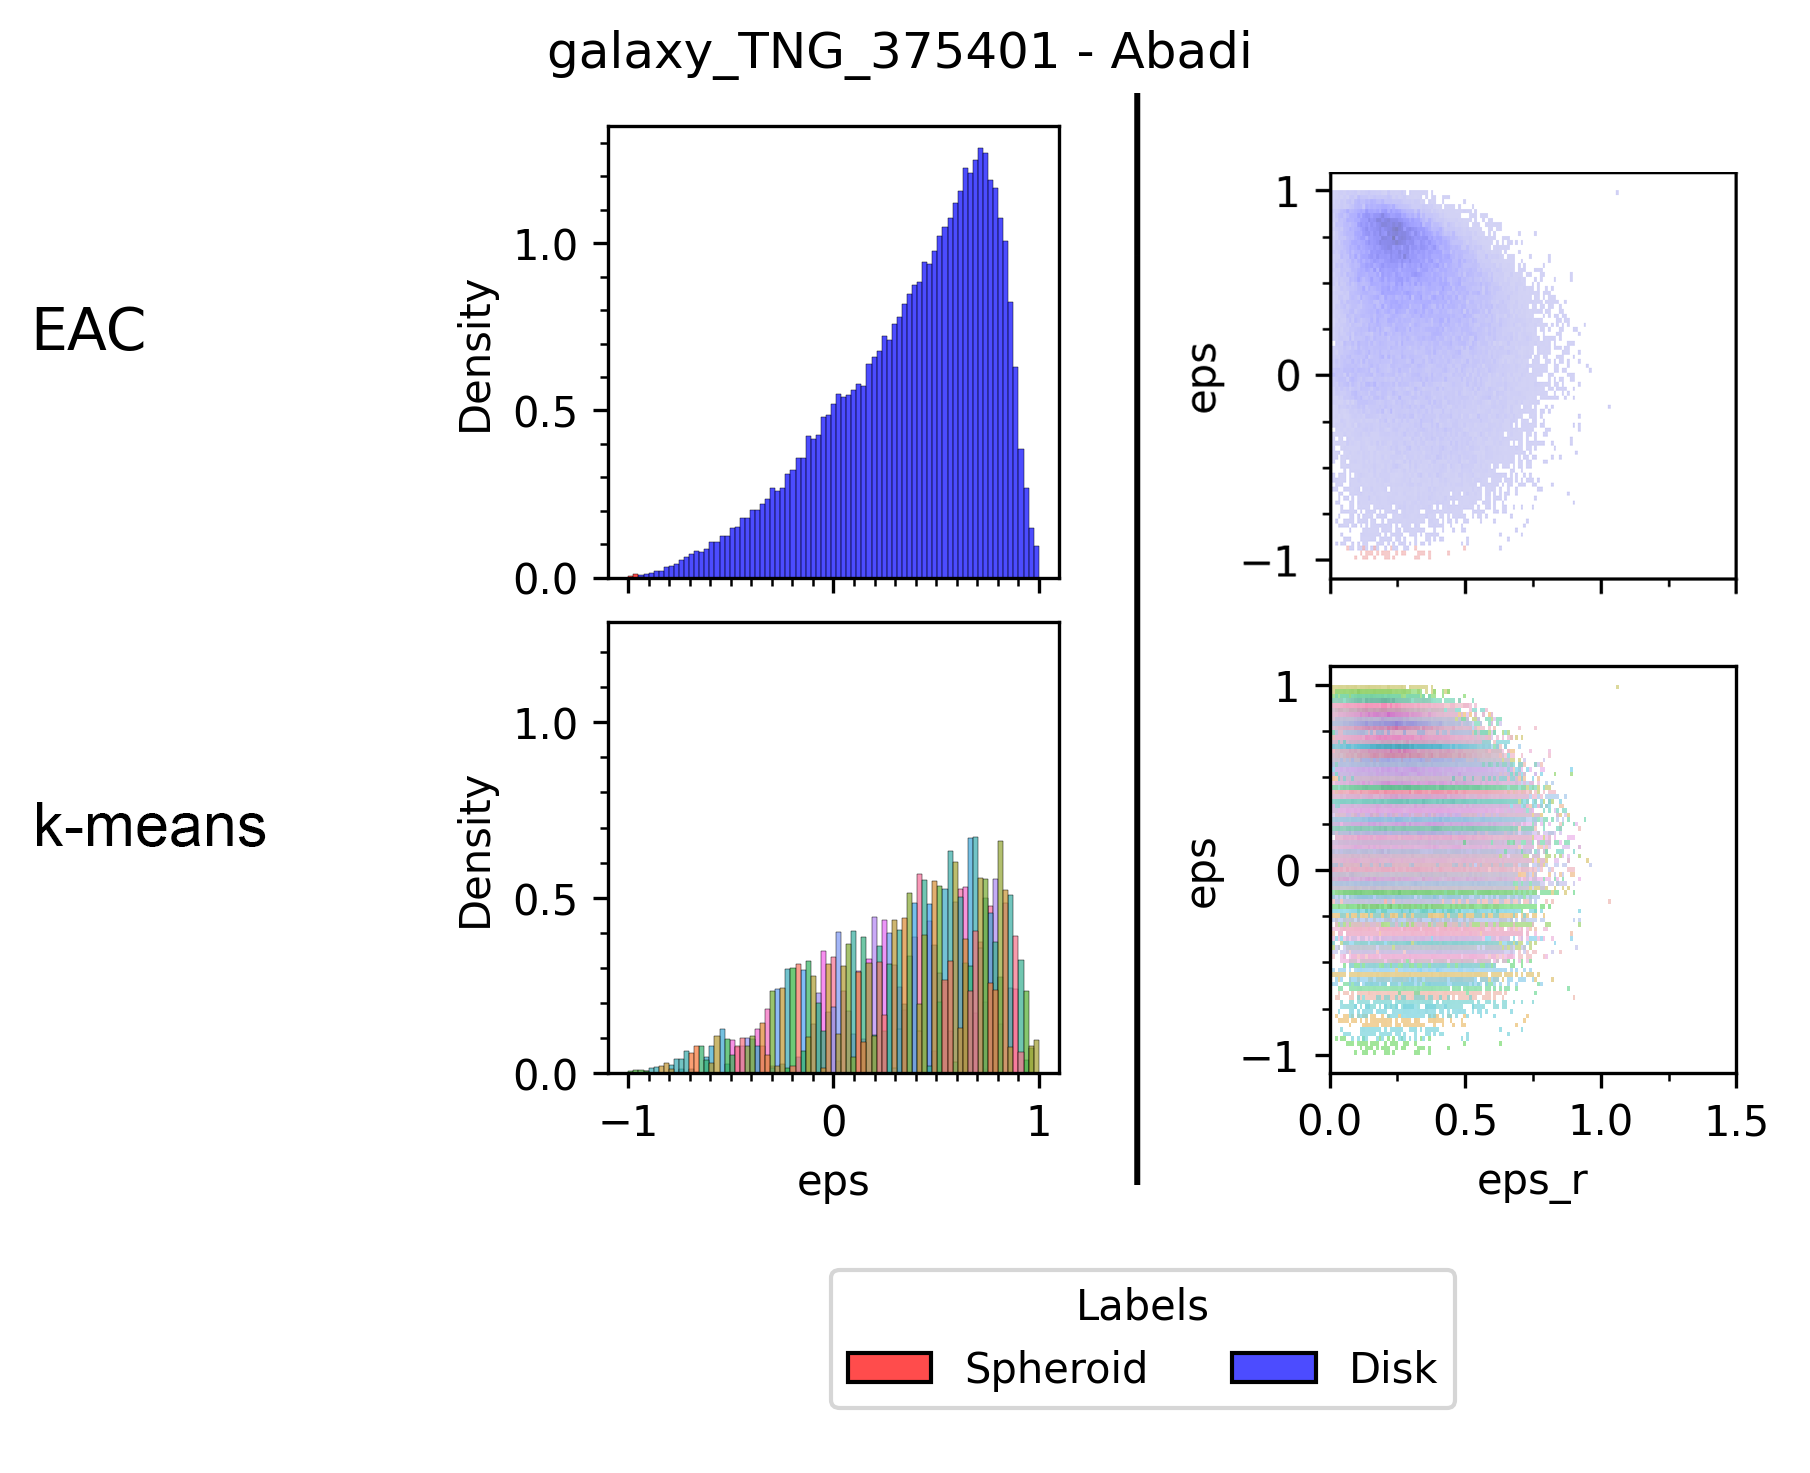
\includegraphics[width=8cm]{evidence accumulation clustering/figures/kmeans example.png}
\end{center}

\note{
- Pinta de estar separados en \textbf{lineas}, esto es porque solo usamos \textbf{eps} \\
- A medida que avanza HC en el ultimo paso del algoritmo de FCM, se van a ir \textbf{uniendo cada clusters adjacente} hasta llegar a los ultimos dos, separados por una linea \\
- Como funciona \textbf{single linkage}: \textbf{minimiza la menor distancia} posible entre dos clusters y los va uniendo \\
%- El mejor resultado hubiera requerido: las partículas alrededor del punto donde la densidad del Disco supera a la del Esferoide en Abadi no hayan compartido muchos clusters que ese punto haya particulas\\
- EAC prioriza en \textbf{fusionar lugares de mayor densidad}, ya que al aumentar la densidad de los puntos las probabilidades de encontrar clusters con metricas de disimilitud pequeñas se incrementa al utilizar single-linkage.  \\
- Por eso se va a un \textbf{extremo} la linea divisora \\
- Por lo feo que da, no vale la pena \textbf{remover outliers}, y ya de entrada no nos parece una buena alternativa \\
}

\end{frame}
\fi




\begin{frame}
\frametitle{AGMM: Detección de $=>$2 componentes}

\begin{center}
    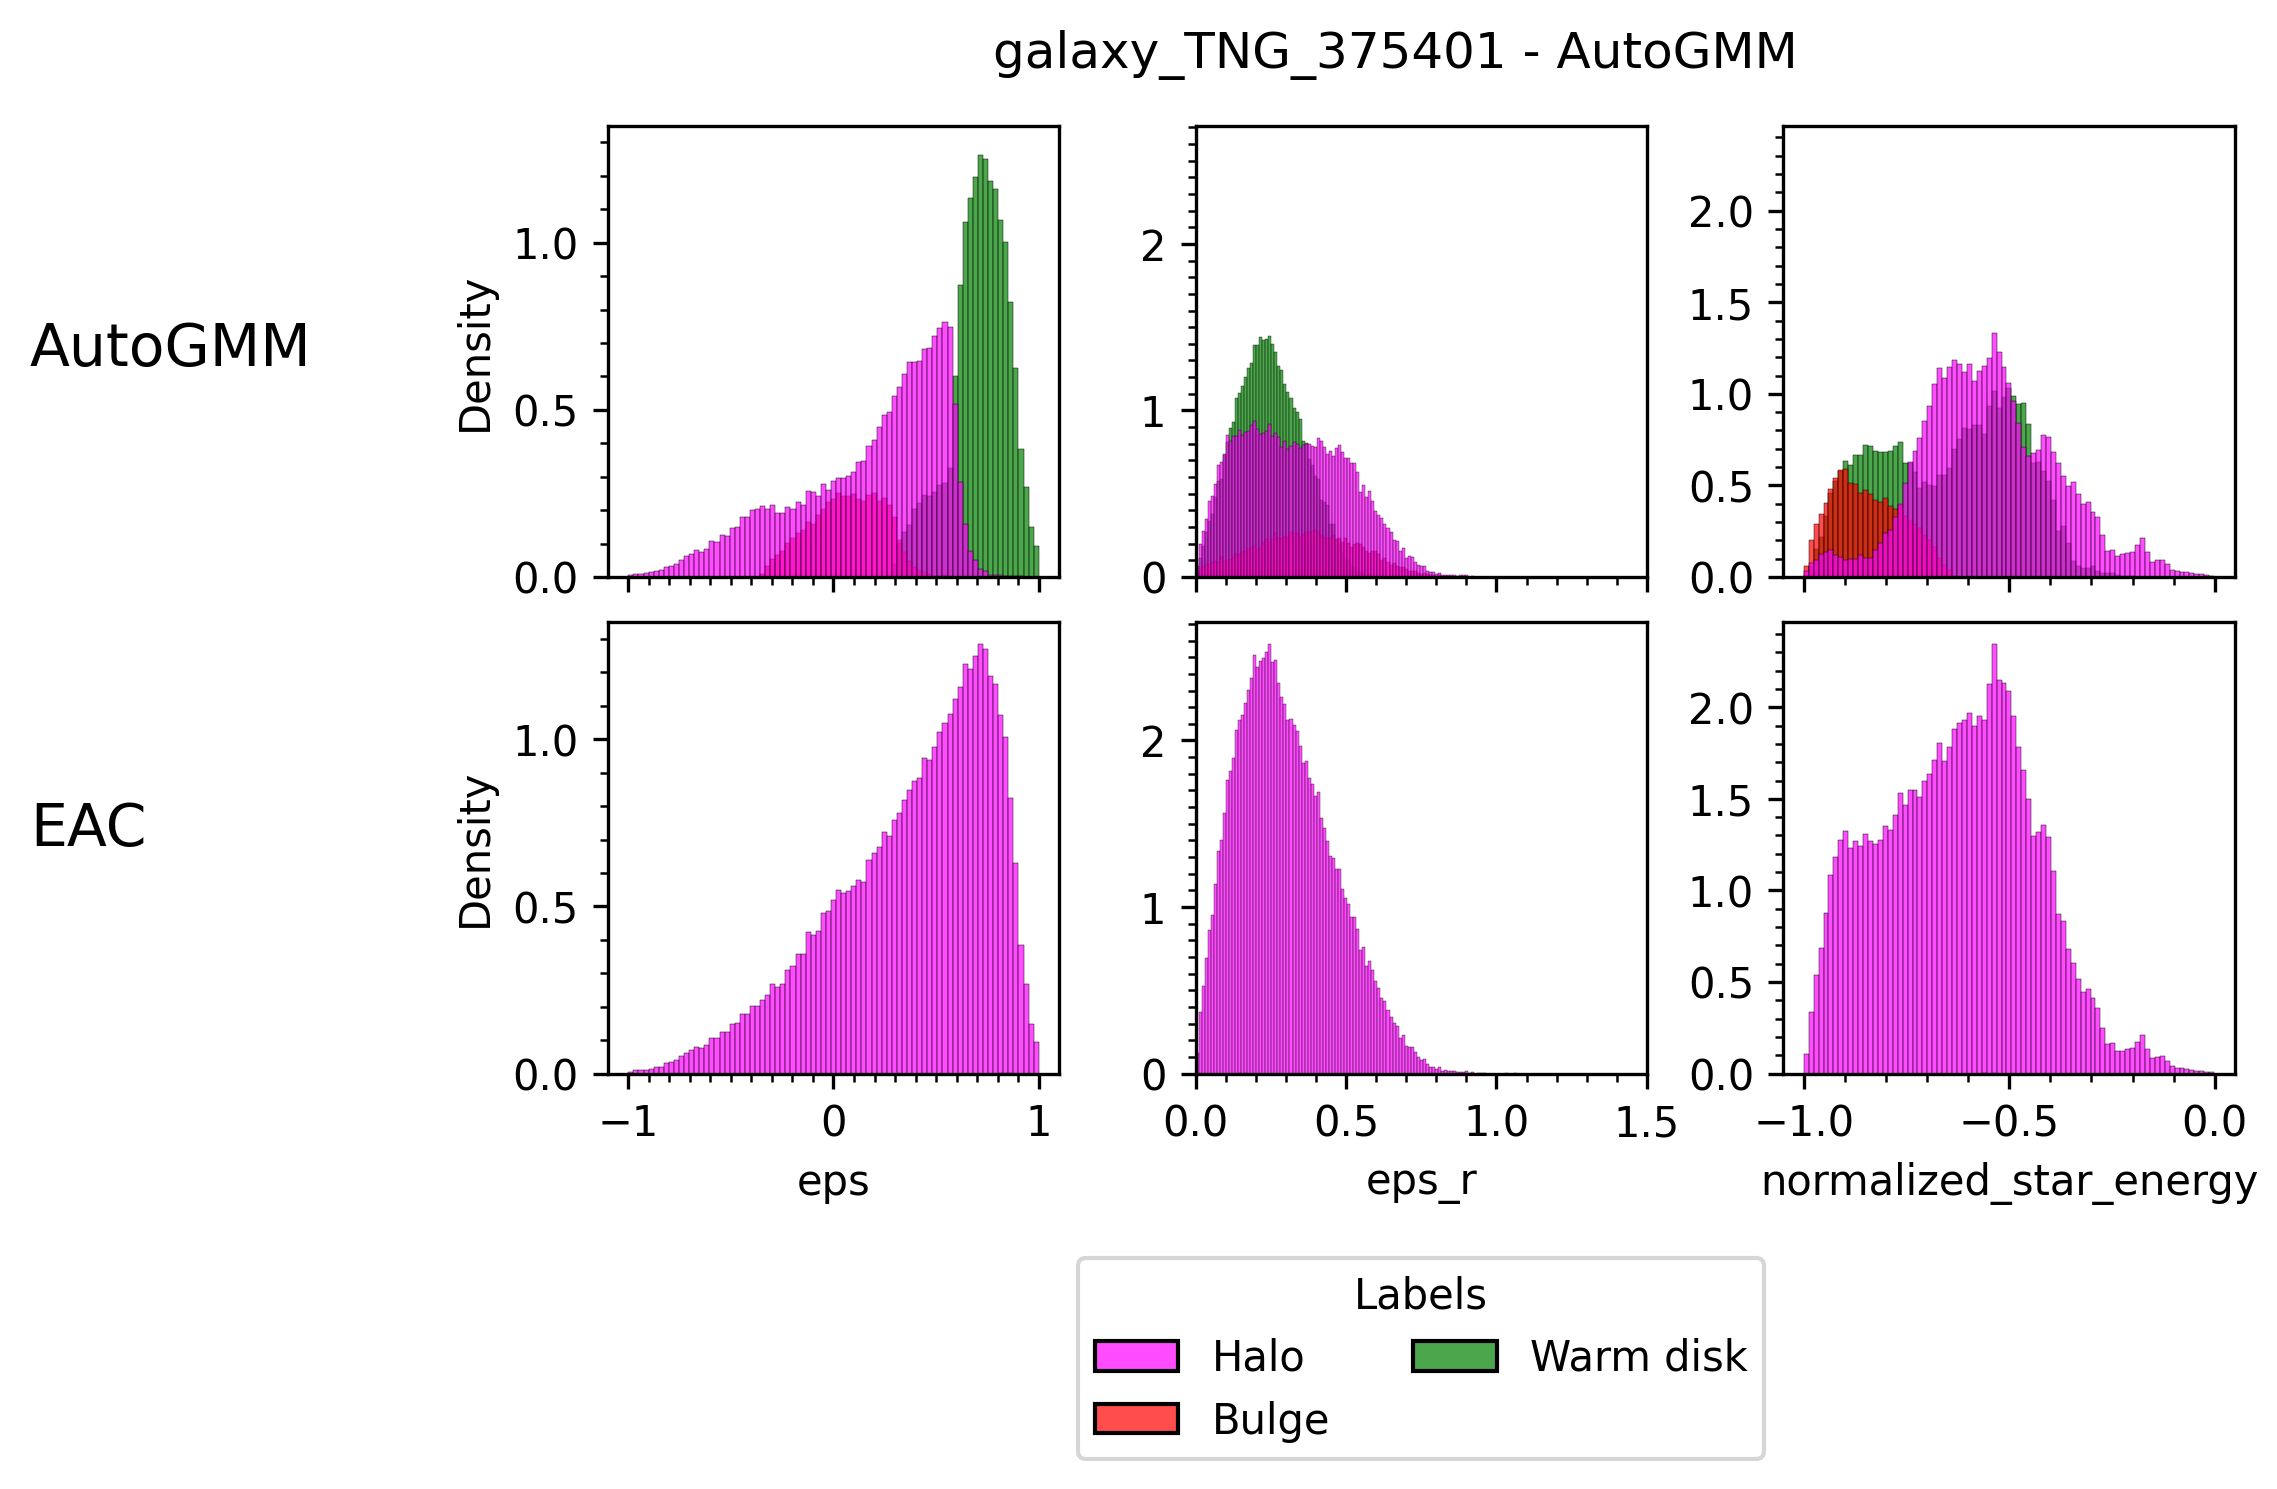
\includegraphics[width=10cm]{evidence accumulation clustering/figures/galaxy_TNG_375401 - eac - agmm - circ histogram.png}
\end{center}

\note{
- N = 100 denuevo \\
- seguimos con alto costo computacional \\
%- aca usamos todas las features, por lo que la razon explicada antes no debe estar aplicando aca \\
- Entendiendo eso, creemos que usar \textbf{valores MUY altos de k} puede entrometerse con encontrar los \textbf{patrones buscados en el dataset}. Resultando de esta manera en una matriz de consenso ruidosa y que \textbf{no captura las co-ocurrencias de los puntos}. \\
- Tambien descubrimos que uno de los experimentos que propone el paper original es \textbf{variar los valores de $k$} utilizados por cada k-means (dentro de las cotas adecuadas) en una misma corrida de \gls{EAC}, siendo esto al parecer \textbf{más robusto} que utilizar un $k$ fijo. \\%Se argumenta que usar un rango amplio de valores puede llegar a tener un efecto de promediado que nos lleve a la identificacion de la estructura verdadera de nuestros datos. \\
- \textbf{Ambas razones} pueden haber sido las causantes de la forma de los resultados obtenidos. Pero de igual manera con los tiempos de computos requeridos por el agoritmo, no habia tiempo para buscar estas cotas como hiperparametros. \\
- Con los experimentos realizados \textbf{no nos es posible recomendar eac} como alternativa para abadi ni para agmm.
}

\end{frame}


\section{Conclusiones}


\begin{frame}
\frametitle{Conclusiones}

\begin{enumerate}
    \item<2-> Resultados de Clustering Jerárquico son cercanos a los de Abadi (entendiendo las limitaciones de usar una sola feature). Pero el alto costo computacional y de memoria en comparacion indican que no es una buena alternativa.
    \item<3-> Clustering Jerárquico obteniendo resultados similares a los de Abadi lo reconfirma, como asi tambien con AGMM.
    \item<4-> Dada que la naturaleza de ciertas subcomponentes alejados a los conceptos usuales de clusterización, los métodos presentados que no asignan una interpretación física a los valores no harán un buen trabajo sobre estas con las features trabajadas.
\end{enumerate}

\note{
\begin{enumerate}
\item<2-> Cabe aclarar que, cuando hablamos de estos algoritmos como posibles \textbf{alternativas} a las ya propuestas en el área, hablamos estrictamente respecto a la tarea de \textbf{encontrar clusters de forma similares}. Es decir, dado que los algoritmos usados en este trabajo son de uso general en minería de datos no es posible para ellos \textbf{etiquetar} cada cluster con la etiqueta correspondiente. \textbf{Responsabilidad} que queda a cargo de quien corre dichos métodos. \\
\item<3-> La \textbf{tendencia} de \gls{HC} a obtener resultados similares a los de Abadi es un \textbf{indicativo extra} del éxito de este último como algoritmo para identificar componentes. \\
\item<4-> El Bulge y el Halo
\end{enumerate}
}

\end{frame}





\begin{frame}
\frametitle{Conclusiones}

\begin{enumerate}
    \setcounter{enumi}{3}
    \item<1-> Fuzzy Clustering también presenta tendencias similares a Abadi, y entendiendo sus limitaciones podría considerarse como una buena alternativa. Pero su comportamiento dista de ser el buscado con mas de 2 clusters para ser considerado una alternativa a AGMM.
    \item<2-> Los resultados obtenidos por Evidence Accumulation Clustering estan lejos de ser similares a los provenientes de Abadi y AGMM. Además, su costo computacional y de memoria son varios ordenes de magnitud mas grandes.
    \item<3-> Las métricas internas utilizadas, Davies–Bouldin y Silhouette, no son de utilidad para analizar el desempeño de algoritmos de clustering en el problema presentado, dada la naturaleza de las componentes reales de una galaxia y como estas difieren de, lo que entienden estas métricas, son buenos clusters.
\end{enumerate}

\note{
\begin{enumerate}
\item<1-> Desincentivando de esta manera cualquier aplicación de este método en la practica. Al menos con la \textbf{implementación utilizada}. \\
\item<3-> Además, \textbf{no fue posible concluir} con ninguno de los métodos explorados si el \textbf{remover outliers} beneficia o no la tarea de buscar los clusters deseados. Dificultando, además, el análisis al buscar un numero variables de clusters dada la variabilidad de la cardinalidad de estos ocasionada por remover partículas estelares de los datos.
\end{enumerate}
}

\end{frame}





\begin{frame}
\frametitle{Trabajo a futuro}

\begin{enumerate}
    \item<1-> Extender el dataset propuesto para realizar experimentos con galaxias espirales.
    \item<2-> Normalización del espacio dinámico antes de correr los metodos vistos.
    \item<3-> Explorar otro tipo de preprocesamientos sobre el espacio dinámico antes de aplicar los métodos propuestos.
    \item<4-> Aplicar diferentes variaciones sobre el primer paso del algoritmo de Evidence Accumulation Clustering.
    \item<5-> Correr Evidence Accumulation Clustering variando los valores de $k$ de cada k-means, buscando la cota inferior y superior de dicha variación como hyperparametros.
    \item<6-> Aplicar otras técnicas de eliminación de outliers.
    \item<7-> Explorar otras features del dataset que podrían contener mas información útil.
    % 
\end{enumerate}

\note{
\begin{enumerate}
\item<2-> (2) En especial \gls{HC} y \gls{FCM}  \\
\item<6-> (6) Sean del area de data mining o algunas mas complejas del area de la astronomia \\
\item<7-> (7) Para encontrar componentes con los métodos propuestos, como la \textbf{edad} o la \textbf{metalicidad}.
\end{enumerate}
}

\end{frame}


\begin{frame}
\frametitle{Contacto}

\begin{center}
Scripts: \href{https://github.com/originalnicodr/GalaxyMLDecompositionThesis}{\textbf{github.com/originalnicodr/GalaxyMLDecompositionThesis}}

    \vspace{3mm}
    \includegraphics<1>[width=10cm]{conclusiones/figures/blank.png}
    \transfade<1-2>
    \includegraphics<2>[width=10cm]{conclusiones/figures/gracias totales.png}
    \vspace{3mm}

\begin{table}[]
\centering
\begin{tabular}{ll}
\faicon{github} \href{https://github.com/originalnicodr}{github.com/originalnicodr} & \faicon{twitter} \href{https://twitter.com/originalnicodr}{twitter.com/originalnicodr}\\
\faicon{linkedin} \href{https://linkedin.com/in/nicolas-uriel-navall}{linkedin.com/in/nicolas-uriel-navall} & \faicon{envelope} \href{mailto:niconavall@gmail.com}{niconavall@gmail.com}\\
\multicolumn{2}{l}{
        \faicon{globe} \href{https://originalnicodr.github.io/}{originalnicodr.github.io}
}
\end{tabular}
\end{table}

\end{center}


\end{frame}

\end{document}